% =====================================================================
% VADEMECUM WISKUNDE – BASISPREAMBULE
% Compacte en consistente LaTeX-setup (A5, ISO-notatie, nette wiskunde)
% =====================================================================

\documentclass[a5paper]{article}

% ---------------------------------------------------------------------
% Taal, typografie & microtypografie
% ---------------------------------------------------------------------
\usepackage[dutch]{babel}
\usepackage[T1]{fontenc}
\usepackage{lmodern}
\usepackage{microtype} % betere letter- en woordspatiëring

% ---------------------------------------------------------------------
% Pagina-instellingen & lay-out
% ---------------------------------------------------------------------
\usepackage[margin=0.5cm]{geometry}
\usepackage{titlesec}
\titlespacing*{\section}{0pt}{*1}{0pt}
\titlespacing*{\subsection}{0pt}{*0.5}{0pt}
\setlength{\textfloatsep}{0pt} % minder witruimte rond figuren/tabellen

% ---------------------------------------------------------------------
% Tekenpakketten & grafische hulpmiddelen
% ---------------------------------------------------------------------
\usepackage{tikz}
\usepackage{tikz-3dplot}
\usetikzlibrary{perspective,positioning,angles,quotes,calc,babel,matrix,decorations.pathreplacing,arrows.meta}

\usepackage{tikzpagenodes}
\usepackage{booktabs, xcolor, colortbl}

% Use the optional short title for marks if provided
\renewcommand{\sectionmark}[1]{%
  \markboth{\MakeUppercase{\thesection\;#1}}{}%
}

% Always place section title in RIGHT margin
\AddToHook{shipout/foreground}{%
  \begin{tikzpicture}[remember picture,overlay]
    \node[
      anchor=north east,
      xshift=1mm, yshift=-3mm,
      rotate=90,
      font=\tiny\sffamily\bfseries,
      text=gray!55
    ] at (current page text area.north east)
    {\leftmark};
  \end{tikzpicture}%
}


\usepackage{pgfplots}
\pgfplotsset{compat=1.18}
\usepackage{graphicx}
\usepackage{adjustbox}
\usepackage{float}

% ---------------------------------------------------------------------
% Wiskunde & symboliek
% ---------------------------------------------------------------------
\usepackage{mathtools}   % laadt amsmath + verbeteringen
\usepackage{amssymb}
\usepackage{bm}          % vette vectoren

% nette differentiaaloperatoren (ISO 80000-2)
\newcommand{\diff}{\mathop{}\!\mathrm{d}}     % totale afgeleide
\newcommand{\pdiff}{\mathop{}\!\partial}      % partiële afgeleide

% veelgebruikte symbolische operatoren
\DeclareMathOperator{\arccot}{arccot}
\DeclareMathOperator{\arcsec}{arcsec}
\DeclareMathOperator{\arccsc}{arccsc}
\DeclareMathOperator{\sech}{sech}
\DeclareMathOperator{\csch}{csch}
\DeclareMathOperator{\sgn}{sgn}

% vectornotatie
\newcommand{\nvec}[1]{\bm n_{#1}}      % normaalvector n_i vet
\newcommand{\norm}[1]{\lVert #1\rVert} % norm

% alle \dfrac standaard in displaystijl
\AtBeginDocument{\renewcommand{\dfrac}{\displaystyle\frac}}

% ---------------------------------------------------------------------
% Tabellen, lijsten & opmaak
% ---------------------------------------------------------------------
\usepackage{array,tabularx,multicol,enumitem}
\usepackage{booktabs} % mooiere tabellen zonder verticale lijnen

% nieuwe kolom voor wiskundige formules in displaystijl
\newcolumntype{E}{>{$\displaystyle}l<{$}}

% ---------------------------------------------------------------------
% Opschriften & hyperlinks
% ---------------------------------------------------------------------
\usepackage{caption}
\usepackage{hyperref}
\hypersetup{
  colorlinks=true,
  linkcolor=blue!50!black,
  urlcolor=blue!50!black
}

% =====================================================================

\begin{document}

%To make all tables compact and visually balanced, add before your tables:
% --- Compact vademecum table style ---
\AtBeginEnvironment{tabular}{\renewcommand{\arraystretch}{1.0}\setlength{\tabcolsep}{3pt}\small}


\title{Vademecum-Formularium Wiskunde}
\author{Ian Claesen}
\date{\today}
\maketitle

\scriptsize
\tableofcontents

\newpage
\normalsize

\section{Algebra}
\subsection{Volgorde van Bewerking}
Haakjes wegwerken, machtsverheffen, worteltrekken, vermenigvuldigen en delen, optellen en aftrekken.

\subsection{Absolute Waarde}
De absolute waarde van een getal $a$ wordt genoteerd als $|a|$ en is altijd positief.
\[
|a| = \begin{cases} 
a & \text{if } a \geq 0 \\
-a & \text{if } a < 0 
\end{cases}\]

\section{Machten en wortels}
\subsection{Machten met Gehele Exponenten}
\renewcommand{\arraystretch}{1.5} % Adjust row height

\[
\begin{array}{|c|c|}
\hline
\begin{array}{l}
\forall a \in ,\forall n \in {\mathbb{N}_0}:{a^n} = \underbrace {a.a.\;...\;.a}_{n\;factoren}\\
\forall a \in {\mathbb{R}}:\;{a^1} = \;a\\
\forall a \in {\mathbb{R}_0}:\;{a^0} = \;1\\
\forall a \in {\mathbb{R}_0},\forall n \in {\mathbb{N}}:\;{a^{ - n}} = \;\frac{1}{{{a^n}}}
\end{array} & \begin{array}{l}
\forall a,b \in {\mathbb{R}_0},\forall m,n \in {\mathbb{Z}}:{a^m} \cdot {a^n} = {a^{m + n}}\\
\frac{{{a^m}}}{{{a^n}}} = {a^{m - n}}\\
{({a^m})^n} = {a^{mn}}\\
{(a.b)^n} = {a^n} \cdot {b^n}\\
{\left( {\frac{a}{b}} \right)^n} = \frac{{{a^n}}}{{{b^n}}}\\
{\left( {\frac{a}{b}} \right)^{ - n}} = {\left( {\frac{b}{a}} \right)^n}
\end{array} \\ 
\hline
\end{array}
\]


\subsection{Vierkantswortel in $\mathbb{R}$}

\[
\begin{array}{|c|c|}
\hline
\begin{array}{l}
\forall a\in\mathbb{R}^+,\forall b\in\mathbb{R}:\\
 b=\sqrt a\Leftrightarrow b^2=a\,\land\,(b\geq0)\\
\forall a,b\in\mathbb{R}^+:\\
\hspace{1cm}\sqrt{a^2}=a\\
\hspace{1cm}\left(\sqrt a\right)^2=a\\
\hspace{1cm}\sqrt{ab} = \sqrt{a} \cdot \sqrt{b}.\\
\hspace{1cm}\sqrt{\frac{a}{b}} = \frac{\sqrt{a}}{\sqrt{b}} \land b \neq 0\\
\end{array} & \begin{array}{l}
\forall a\in\mathbb{R}:\\
\sqrt{a^2} = \left|a\right| \implies 
\begin{cases} 
    \sqrt{a^2} = a & \text{als } a \geq 0, \\ 
    \sqrt{a^2} = -a & \text{als } a \leq 0.
\end{cases}
\end{array} \\ 
\hline
\end{array}
\]

\subsection{N-de machtswortel in $\mathbb{R}$}
\[
\begin{array}{|c|c|}
\hline
\begin{array}{l}
n\,\,even\Rightarrow\sqrt[n]{a^n}=\left|a\right|\rightarrow\left\{\begin{matrix}\sqrt[n]{a^n}=a&\land\, a\geq0\\\sqrt[n]{a^n}=-a&\land\, a\le0\\\end{matrix}\right.\,\\
n\,\, oneven\Rightarrow\sqrt[n]{a^n}=a
\end{array} & \begin{array}{l}
\forall a,b\in\mathbb{R}_0^+,\forall m,n\in\mathbb{N}_0:\\
\sqrt[n]{a^n}=a\\
\left(\sqrt[n]{a}\right)^n=a\\
\sqrt[n]{ab}=\sqrt[n]{a}.\sqrt[n]{b}\\
\sqrt[n]{\frac{a}{b}}=\frac{\sqrt[n]{a}}{\sqrt[n]{b}}\\
\sqrt[m]{\sqrt[n]{a}}=\sqrt[m.n]{a}
\end{array} \\ 
\hline
\end{array}
\]

\newpage

\subsection{\texorpdfstring{$\frac{m}{n}$-de machtswortel in $\mathbb{R}$}{m/n-de machtswortel in R}}
\[
\begin{array}{|c|c|}
\hline
\begin{array}{l}
\forall a\in\mathbb{R}_0^+,\forall m\in\mathbb{Z},\forall n\in\mathbb{N}_0:a^\frac{m}{n}=\sqrt[n]{a^m}
\end{array} & \begin{array}{l}
\forall a,b\in\mathbb{R}_0^+,\forall m,n\in\mathbb{Q}:\\
a^m.a^n=a^{m+n}\\
\frac{a^m}{a^n}=a^{m-n}\\
\left(a^m\right)^n=a^{m.n}\\
\left(a.b\right)^m=a^m.b^m\\
\left(\frac{a}{b}\right)^m=\frac{a^m}{b^m}
\end{array} \\ 
\hline
\end{array}
\]

\section{Veeltermen}
\subsection{Vierkantsvergelijking}
$Een\:vierkantsvergelijking\:is\:van\:de\:vorm:\:ax^2 + bx + c = 0\:,\:met\:D=b^2 - 4ac $

\renewcommand{\arraystretch}{1.5} % Adjust row height
\[
\begin{array}{|c|c|}
\hline
x\in{\displaystyle \mathbb {R} } & x\in{\displaystyle \mathbb {C} } \\ 
\hline
x_{1,2} = \frac{-b \pm \sqrt{D}}{2a} \quad  & x_{1,2} = \frac{-b \pm i\sqrt{-D}}{2a} \quad \\ 
\hline
P = \frac{c}{a} = x_1 \cdot x_2\:,\:S = -\frac{b}{a} = x_1 + x_2 &  \\ 
\hline
ax^2 + bx + c = a(x - x_1)(x - x_2) = a(x^2 - Sx + P) & \\
\hline
\end{array}
\]

\subsection{Merkwaardige Producten en Ontbinding in Factoren}
\[
\begin{array}{|l|l|}
\hline
(a\pm b)^2 = a^2 \pm 2ab + b^2 \\ 
\hline
{\left( {a \pm b} \right)^3} = {a^3} \pm 3{a^2}b + 3a{b^2} \pm {b^3} \\
\hline
{\left( {a + b} \right)^n} = {a^n} + C_n^1{a^{n - 1}}b + C_n^2{a^{n - 2}}{b^2} + ... + C_n^{n - 1}{a^2}{b^{n - 1}} + {b^n}\quad  \wedge \quad C_n^p = \frac{{n!}}{{\left( {n - p} \right)!p!}} \\
\hline
{a^2} - {b^2} = \left( {a + b} \right)\left( {a - b} \right) \\
\hline
{a^3} - {b^3} = \left( {a - b} \right)\left( {{a^2} + ab + {b^2}} \right) \\
\hline
{a^n} - {b^n} = \left( {a - b} \right)\left( {{a^{n - 1}} + {a^{n - 2}}b + {a^{n - 3}}{b^2} + ... + a{b^{n - 2}} + {b^{n - 1}}} \right) \\
\hline
{a^3} + {b^3} = \left( {a + b} \right)\left( {{a^2} - ab + {b^2}} \right) \\
\hline
{a^{2n + 1}} + {b^{2n + 1}} = \left( {a + b} \right)\left( {{a^{2n}} - {a^{2n - 1}}b + {a^{2n - 2}}{b^2} - {a^{2n - 3}}{b^3} + ... - a{b^{2n - 1}} + {b^{2n}}} \right) \\
\hline
\end{array}
\]

\subsection{Deelbaarheid in $\mathbb{R} [x]$}

\[
V(x),\:D(x),\:Q(x),\:R(x)\:\in \mathbb{R}[x] : \frac{V(x)}{D(x)}= Q(x) + R(x)
\]

\[
Reststelling\; : \;\frac{V(x)}{x-a}\Rightarrow R(x)=V(a)
\]

\newpage

\subsection{Euclidische Deling}
We gaan de derdegraadsveelterm $2x^3 + 3x^2 - 4x + 5$ delen door de eerstegraadsveelterm $x + 2$ met behulp van de praktische werkwijze van lange deling.

\[
\begin{array}{r !{\vrule width 1pt} l}
   2x^3 + 3x^2 - 4x + 5\; & x + 2 \\
  \noalign{\hrule height 1pt}
  -(2x^3 + 4x^2 + 0x + 0) & 2x^2 \\
  \hline
  \textcolor{red}{- 1x^2 - 4x + 5\;} & \\
  \textcolor{red}{-(-1x^2 - 2x + 0)} & \textcolor{red}{-x} \\
  \hline
  \textcolor{blue}{-2x + 5} & \\
  \textcolor{blue}{-(-2x - 4)} & \textcolor{blue}{-2} \\
  \hline
  \textcolor{purple}{9} & 
\end{array}
\]

We kunnen de deling als volgt uitdrukken:
\[
2x^3 + 3x^2 - 4x + 5 = (x + 2)(2x^2 - x - 2) + 9
\]

De rest is $9$, wat een graad heeft die kleiner is dan de graad van de deler $x + 2$.


\subsection{Schema van Horner}
\[
\frac{(3x^3-5x^2+10x-5)}{(x-2)}=3x^2+1x+12+\frac{19}{(x-2)}
\]

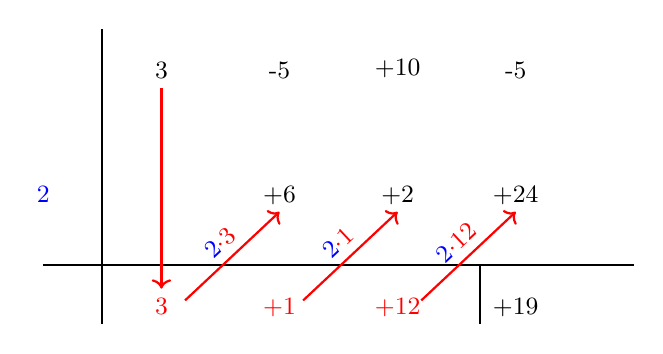
\begin{tikzpicture}[scale=1.5, every node/.style={font=\small}]
    % Draw the axes
    \draw[thick, -] (-0.5, 0) -- (4.5, 0); % Horizontal axis
    \draw[thick, -] (0, -0.5) -- (0, 2); % Vertical axis

    % Top row numbers
    \node[above] at (0.5, 1.5) {3};
    \node[above] at (1.5, 1.5) {-5};
    \node[above] at (2.5, 1.5) {+10};
    \node[above] at (3.5, 1.5) {-5};

    % Bottom row numbers
	\node[below] at (0.5, -0.2) {\textcolor{red}{3}};
	\node[below] at (1.5, -0.2) {\textcolor{red}{+1}};
	\node[below] at (2.5, -0.2) {\textcolor{red}{+12}};
    \node[below] at (3.5, -0.2) {+19};

    % Draw vertical arrow for the first step
    \draw[->, thick, red] (0.5, 1.5) -- (0.5, -0.2);
    \node[below,blue] at (-0.5, 0.75) {$2$};

    % Draw horizontal arrows with blue 2 in labels
    \draw[->, thick, red] (0.7, -0.3) -- (1.5, 0.45)
        node[midway, above, red, sloped] {\textcolor{blue}{2}$\cdot3$};
    \node[below] at (1.5, 0.75) {+6};

    \draw[->, thick, red] (1.7, -0.3) -- (2.5, 0.45)
        node[midway, above, red, sloped] {\textcolor{blue}{2}$\cdot1$};
    \node[below] at (2.5, 0.75) {+2};

    \draw[->, thick, red] (2.7, -0.3) -- (3.5, 0.45)
        node[midway, above, red, sloped] {\textcolor{blue}{2}$\cdot12$};
    \node[below] at (3.5, 0.75) {+24};

    \draw[thick, -] (3.2, 0) -- (3.2, -0.5); % Vertical axis
\end{tikzpicture}


\newpage

\section{Complexe getallen}
\subsection{Rechthoekige coordinaten}
\[
\begin{array}{|l|l|}
\hline
\textbf{Bewerking} & \textbf{Formule} \\ \hline
Optelling/Aftrekking & (a + j.b) \pm (c + j.d) = (a + c) \pm j(b + d) \\ \hline
Vermenigvuldiging & (a + j.b) \cdot (c + j.d) = (ac - bd) + j(ad + bc) \\ \hline
Deling & 
\frac{(a + j.b)}{(c + j.d)} = \frac{(a + j.b) \cdot (c - j.d)}{(c + j.d) \cdot (c - j.d)} = \left( \frac{ac + bd}{c^2 + d^2} \right) + j \left( \frac{bc - ad}{c^2 + d^2} \right) \\ \hline
Toegevoegde\:van & \overline{(a + j.b)} = (a - j.b) \\
& \overline{Z_1 + Z_2} = \overline{Z_1} + \overline{Z_2}, \quad \overline{Z_1 \cdot Z_2} = \overline{Z_1} \cdot \overline{Z_2} \\ \hline
Inverse & z = a + bi \implies z^{-1} = \frac{a - bi}{a^2 + b^2} \\ \hline
Wortel & 
\sqrt{a} \; \wedge \; a < 0 \implies \sqrt{a} = \pm i\sqrt{-a} \\ 
& \sqrt{a + bi} = x + yi \iff (x + yi)^2 = a + bi \\ \hline
Macht & 
(a + bi)^0 = 1 \quad \forall n \in \mathbb{N}_0: \\
& (a + bi)^n = (a + bi) \cdot (a + bi) \cdots (a + bi) \\ \hline
Machten\:of\:i & i^1 = i, \quad i^2 = -1, \quad i^3 = -i, \quad i^4 = 1 \\ \hline
\end{array}
\]

\subsection{Poolcoördinaten}
\[z = a + i.b = r\left( {\cos (\varphi ) + i.\sin (\varphi )} \right) = r\angle \varphi ,\quad \tan (\varphi ) = \frac{b}{a},\quad r = \sqrt {{a^2} + {b^2}} \]
\[
\begin{array}{|l|l|}
\hline
\textbf{Bewerking} & \textbf{Formule} \\
\hline
Vermenigvuldiging & {z_1} \cdot {z_2} = {r_1} \cdot {r_2}\angle {\varphi _1} + {\varphi _2} \\
\hline
Deling & \frac{{{z_1}}}{{{z_2}}} = \frac{{{r_1}\angle {\varphi _1}}}{{{r_2}\angle {\varphi _2}}} = \frac{{{r_1}}}{{{r_2}}}\angle {\varphi _1} - {\varphi _2} \\
\hline
Inverse & {z^{ - 1}} = \frac{1}{r}\angle  - \varphi  \\ \hline
Macht & {z^n} = {r^n}\left[ {\cos \left( {n \cdot \varphi } \right) + i\sin \left( {n \cdot \varphi } \right)} \right]\quad n \in {\displaystyle \mathbb {N} }\\
\hline
Wortel & 
\sqrt {r(\cos \varphi  + i\sin \varphi )}  =  \pm \sqrt r \left( {\cos \frac{\varphi }{2} + i\sin \frac{\varphi }{2}} \right)\\
\hline
\multicolumn{2}{|c|}{\sqrt[n]{{r\left( {\cos \varphi  + i\sin \varphi } \right)}} = \sqrt[n]{r}\left( {\cos \frac{{\varphi  + k \cdot 2\pi }}{n} + i\sin \frac{{\varphi  + k \cdot 2\pi }}{n}} \right)\quad  \wedge \quad k = 0,1, \cdots ,n - 1} \\
\hline
 \end{array}
\]

\newpage

\section{Goniometrie}
\subsection{De Goniometrische Cirkel}

\begin{center}
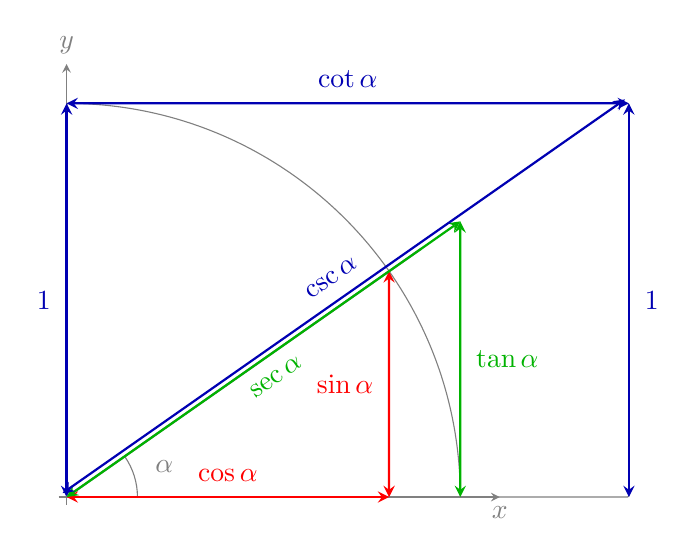
\begin{tikzpicture}[>=stealth,scale=5,
  sincos/.style ={red,thick},
  tansec/.style ={green!70!black,thick},
  cotcsc/.style ={blue!70!black,thick},
  guide/.style  ={black!50}
]
  % ----- angle parameter -----
  \def\ang{35} % degrees

  % ----- basic trig values -----
  \pgfmathsetmacro{\cx}{cos(\ang)}
  \pgfmathsetmacro{\sx}{sin(\ang)}
  \pgfmathsetmacro{\tx}{tan(\ang)}
  \pgfmathsetmacro{\cotx}{cot(\ang)}
  \pgfmathsetmacro{\secx}{sec(\ang)}
  \pgfmathsetmacro{\cscx}{cosec(\ang)} % same as csc

  % ----- reference objects: axes and quarter of unit circle -----
  \draw[guide,->] (-0.02,0) -- (1.1,0) node[below] {$x$};
  \draw[guide,->] (0,-0.02) -- (0,1.1) node[above] {$y$};
  % quarter circle only (first quadrant)
  \draw[guide] (1,0) arc[start angle=0,end angle=90,radius=1];

  % optional rectangle lines (only within first quadrant)
  \draw[guide,rounded corners=0.5pt]
    (0,0) rectangle (\cotx,1);

  % vertical “1” bars (left & right)
  \draw[cotcsc,<->] (0,0) -- (0,1) node[midway,left=2pt] {$1$};
  \draw[cotcsc,<->] (\cotx,0) -- (\cotx,1) node[midway,right=2pt] {$1$};

  % ----- angle ray -----
  \draw[guide,thick] (0,0) -- (\ang:1.1);     % ray
  \draw[guide] (0.18,0) arc[start angle=0,end angle=\ang,radius=0.18];
  \node[guide] at ({0.26*cos(\ang/2)},{0.26*sin(\ang/2)}) {$\alpha$};

  % points
  \coordinate (U) at (\cx,\sx);               % on unit circle
  \coordinate (X1) at (1,\tx);                % intersect x=1 line
  \coordinate (Y1) at (\cotx,1);              % intersect y=1 line

  % ----- cos and sin -----
  \draw[sincos,<->] (0,0) -- (\cx,0) node[midway,above=2pt] {\(\cos\alpha\)};
  \draw[sincos,<->] (\cx,0) -- (U) node[midway,left=2pt] {\(\sin\alpha\)};

  % ----- tan and sec (x=1) -----
  \draw[tansec,<->] (1,0) -- (X1) node[midway,right=2pt] {\(\tan\alpha\)};
  \draw[tansec,<->] (0,0) -- (X1) node[midway,below=2pt,sloped] {\(\sec\alpha\)};

  % ----- cot and csc (y=1) -----
  \draw[cotcsc,<->] (0,1) -- (Y1) node[midway,above=2pt] {\(\cot\alpha\)};
  \draw[cotcsc,<->] (-0.01,0.01) -- (\cotx-0.01,1+0.01) node[midway,above=2pt,sloped] {\(\csc\alpha\)};
\end{tikzpicture}
\end{center}


\subsection{formules uit de goniometrie}

\begin{center}
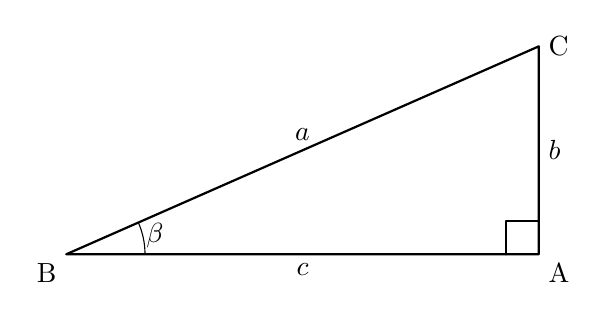
\begin{tikzpicture}[scale=1.2, line cap=round, line join=round, >=stealth]
  % vertices
  \coordinate (B) at (0,0);
  \coordinate (A) at (5,0);
  \coordinate (C) at (5,2.2);

  % triangle
  \draw[thick] (B) -- (A) -- (C) -- cycle;

  % right-angle marker at A (inside the triangle)
  \draw[thick]
    ($(A)+(-0.35,0)$) -- ($(A)+(-0.35,0.35)$) -- ($(A)+(0,0.35)$);

  % angle beta at B
  \pic [draw, "$\beta$", angle radius=10mm, angle eccentricity=1.15]
       {angle=A--B--C};

  % side labels
  \node[below]           at ($(A)!0.5!(B)$) {$c$};
  \node[right]           at ($(A)!0.5!(C)$) {$b$};
  \node[above,sloped]    at ($(B)!0.5!(C)$) {$a$};

  % vertex labels
  \node[below left]  at (B) {B};
  \node[below right] at (A) {A};
  \node[right]       at (C) {C};
\end{tikzpicture}

\end{center}

\[\begin{array}{|c|c|}
\hline
\begin{array}{*{20}{c}}
{\csc \beta }&{sec\beta }&{\cot \beta }\\
 \leftarrow & \leftarrow & \leftarrow \\
{os}&{as}&{oa}\\
 \to & \to & \to \\
{\sin \beta }&{\cos \beta }&{\tan \beta }
\end{array}

& % Scheiding van de twee kolommen

\begin{array}{l}
\text{waarin:} 
\left\{
\begin{aligned}
& o: \text{ overstaande rechthoekszijde} \\
& s: \text{ schuine zijde (hypotenusa)} \\
& a: \text{ aanliggende rechthoekszijde}
\end{aligned}
\right.
\end{array} \\ 
\hline
\end{array}
\]

\[
\begin{array}{|c|c|}
\hline
\text{sin} \, \beta = \frac{b}{a} \hspace{1cm} \text{cos} \, \beta = \frac{c}{a} \hspace{1cm} \text{tan} \, \beta = \frac{b}{c} \\
\hline
\text{csc} \, \beta = \frac{a}{b} \hspace{1cm} \text{sec} \, \beta = \frac{a}{c} \hspace{1cm} \text{cot} \, \beta = \frac{c}{b} \\
\hline
\text{tan} \, \alpha = \frac{\sin \alpha}{\cos \alpha} \hspace{1cm} \text{cot} \, \alpha = \frac{\cos \alpha}{\sin \alpha} \hspace{1cm} \text{cot} \, \alpha = \frac{1}{\tan \alpha} \\
\hline
\text{sec} \, \alpha = \frac{1}{\cos \alpha} \hspace{1cm} \text{csc} \, \alpha = \frac{1}{\sin \alpha}\\
\hline
\end{array}
\]

\[
\boxed{\sin^2{\alpha} + \cos^2{\alpha} = 1} \hspace{1cm}
\boxed{\tan^2{\alpha} + 1 = \sec^2{\alpha}} \hspace{1cm}
\boxed{1 + \cot^2{\alpha} = \csc^2{\alpha}}
\]

\newpage
\subsection{Verwante hoeken}

\begin{center}
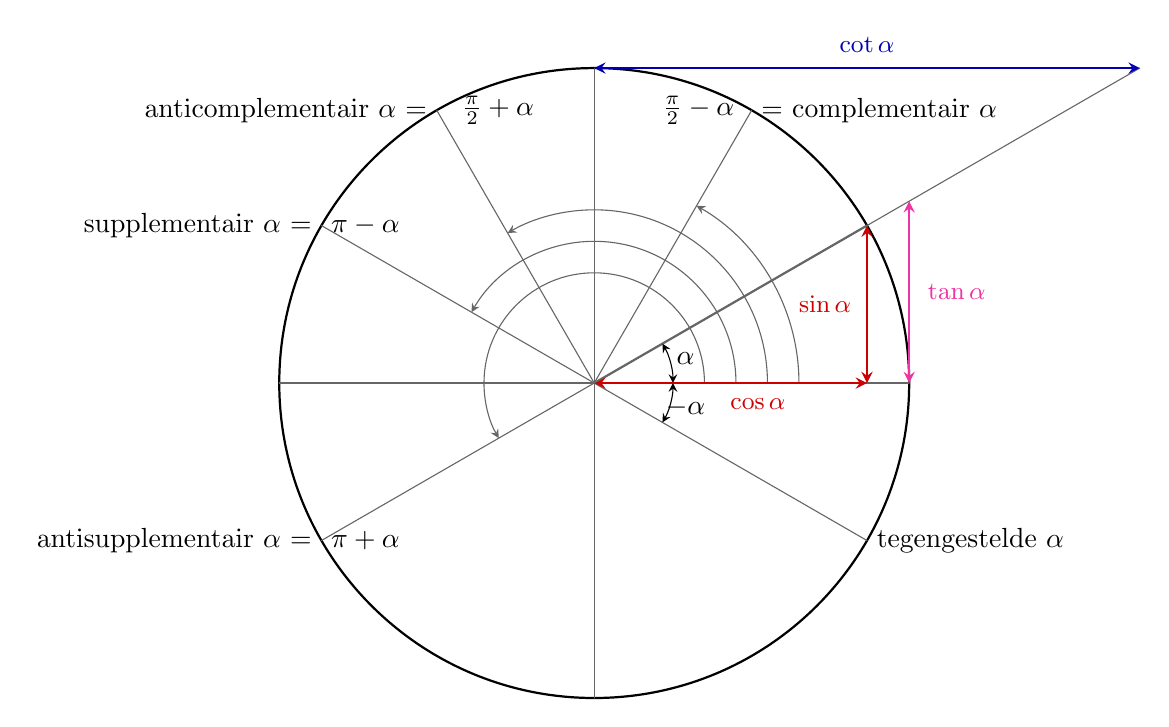
\begin{tikzpicture}[scale=4, line cap=round, line join=round, >=stealth]
  % styles
  \tikzset{
    guide/.style={black!60},
    labg/.style={guide, font=\footnotesize},
    sincos/.style={red!80!black, thick},
    tansec/.style={magenta!80, thick},
    cotcsc/.style={blue!70!black, thick}
  }

  % ----- parameter -----
  \def\ang{30} % degrees

  % ----- base points (avoid commas in \pic arguments) -----
  \coordinate (O) at (0,0);
  \coordinate (X) at (1,0);
  \coordinate (Y) at (0,1);
  \coordinate (P) at (\ang:1);          % on unit circle, angle α
  \coordinate (P90m) at (90-\ang:1);
  \coordinate (P90p) at (90+\ang:1);
  \coordinate (P180m) at (180-\ang:1);
  \coordinate (P180) at (180:1);
  \coordinate (P180p) at (180+\ang:1);
  \coordinate (Pneg) at (-\ang:1);

  % trig numbers (for sin/cos/tan/cot)
  \pgfmathsetmacro{\cx}{cos(\ang)}
  \pgfmathsetmacro{\sx}{sin(\ang)}
  \pgfmathsetmacro{\tx}{tan(\ang)}
  \pgfmathsetmacro{\cotx}{cot(\ang)}

  % ----- unit circle & axes -----
  \draw[thick] (O) circle[radius=1];
  \draw[guide] (-1,0) -- (1,0);
  \draw[guide] (0,-1) -- (0,1);

  % rays
  \draw[guide,thick] (O) -- (P);
  \foreach \Q in {P90m,P90p,P180m,P180p,Pneg} \draw[guide] (O) -- (\Q);

  % angle labels (now using named coords)
  \pic[draw,<->,"$\alpha$",angle radius=10mm,angle eccentricity=1.2]
      {angle=X--O--P};
  \pic [draw,->,labg,angle radius=26mm,angle eccentricity=1.2]
      {angle=X--O--P90m};
  \pic [draw,->,labg,angle radius=22mm,angle eccentricity=1.2]
      {angle=X--O--P90p};
  \pic[draw,->,labg,angle radius=18mm,angle eccentricity=1.2]
      {angle=X--O--P180m};
  \pic[draw,->,labg,angle radius=14mm,angle eccentricity=1.2]
      {angle=X--O--P180p};
  \pic[draw,<->,"$-\alpha$",angle radius=10mm,angle eccentricity=1.2]
      {angle=Pneg--O--X};

  % outside captions
  \node[anchor=east]  at (P180m) {supplementair $\alpha$ = };
  \node[anchor=west]  at (P180m) { $ \pi-\alpha$};

  \node[anchor=east]  at (P180p) {antisupplementair $\alpha$ =};
  \node[anchor=west]  at (P180p) { $  \pi+\alpha$};

  \node[anchor=west]  at (Pneg) {tegengestelde $\alpha$};

  \node[anchor=east] at (P90p) {anticomplementair $\alpha$ =};
  \node[anchor=west]  at (P90p) { $\;\; \frac{\pi}{2}+\alpha$};

  \node[anchor=east]  at (P90m) { $\frac{\pi}{2}-\alpha \;$};
  \node[anchor=west]  at (P90m) {= complementair $\alpha$};

  % sin & cos for α
  \coordinate (U) at (\cx,\sx);
  \draw[sincos,<->] (O) -- (\cx,0) node[pos=0.6 ,below=2pt] {\small $\cos\alpha$};
  \draw[sincos,<->] (\cx,0) -- (U)    node[midway,left=2pt] {\small $\sin\alpha$};

  % tangent (x=1) & cotangent (y=1)
  \draw[guide] (O) -- ({max(1.25,\cotx)},1);
  \draw[tansec,<->] (1,0) -- (1,\tx) node[midway,right=3pt] {\small $\tan\alpha$};
  \draw[cotcsc,<->] (0,1) -- (\cotx,1) node[midway,above=2pt] {\small $\cot\alpha$};
\end{tikzpicture}
\end{center}

\[
\begin{array}{|l|l|l|}
\hline
\text{gelijkehoeken} & \text{supplementairehoeken} & \text{complementairehoeken} \\
\hline
\sin{\left(\alpha + k2\pi\right)} = \sin{\alpha} & \sin{\left(\pi - \alpha\right)} = \sin{\alpha} & \sin{\left(\frac{\pi}{2} - \alpha\right)} = \cos{\alpha} \\
\cos{\left(\alpha + k2\pi\right)} = \cos{\alpha} & \cos{\left(\pi - \alpha\right)} = -\cos{\alpha} & \cos{\left(\frac{\pi}{2} - \alpha\right)} = \sin{\alpha} \\
\tan{\left(\alpha + k2\pi\right)} = \tan{\alpha} & \tan{\left(\pi - \alpha\right)} = -\tan{\alpha} & \tan{\left(\frac{\pi}{2} - \alpha\right)} = \cot{\alpha} \\
\cot{\left(\alpha + k2\pi\right)} = \cot{\alpha} & \cot{\left(\pi - \alpha\right)} = -\cot{\alpha} & \cot{\left(\frac{\pi}{2} - \alpha\right)} = \tan{\alpha} \\
\sec{\left(\alpha + k2\pi\right)} = \sec{\alpha} & \sec{\left(\pi - \alpha\right)} = -\sec{\alpha} & \sec{\left(\frac{\pi}{2} - \alpha\right)} = \csc{\alpha} \\
\csc{\left(\alpha + k2\pi\right)} = \csc{\alpha} & \csc{\left(\pi - \alpha\right)} = \csc{\alpha} & \csc{\left(\frac{\pi}{2} - \alpha\right)} = \sec{\alpha} \\
\hline
\end{array}
\]

\[
\begin{array}{|l|l|l|}
\hline
\text{tegengesteldehoeken} & \text{antisupplementairehoeken} & \text{anticomplementairehoeken} \\
\hline
\sin{\left(-\alpha\right)} = -\sin{\alpha} & \sin{\left(\pi + \alpha\right)} = -\sin{\alpha} & \sin{\left(\frac{\pi}{2} + \alpha\right)} = \cos{\alpha} \\
\cos{\left(-\alpha\right)} = \cos{\alpha} & \cos{\left(\pi + \alpha\right)} = -\cos{\alpha} & \cos{\left(\frac{\pi}{2} + \alpha\right)} = -\sin{\alpha} \\
\tan{\left(-\alpha\right)} = -\tan{\alpha} & \tan{\left(\pi + \alpha\right)} = \tan{\alpha} & \tan{\left(\frac{\pi}{2} + \alpha\right)} = -\cot{\alpha} \\
\cot{\left(-\alpha\right)} = -\cot{\alpha} & \cot{\left(\pi + \alpha\right)} = \cot{\alpha} & \cot{\left(\frac{\pi}{2} + \alpha\right)} = -\tan{\alpha} \\
\sec{\left(-\alpha\right)} = \sec{\alpha} & \sec{\left(\pi + \alpha\right)} = -\sec{\alpha} & \sec{\left(\frac{\pi}{2} + \alpha\right)} = -\csc{\alpha} \\
\csc{\left(-\alpha\right)} = -\csc{\alpha} & \csc{\left(\pi + \alpha\right)} = -\csc{\alpha} & \csc{\left(\frac{\pi}{2} + \alpha\right)} = \sec{\alpha} \\
\hline
\end{array}
\]

\newpage

\subsection{Belangrijke goniometrische waarden}
\[
\begin{array}{|c|c|c|c|c|c|c|c|c|c|}
\hline
\text{Angle} & 0^\circ & 30^\circ & 45^\circ & 60^\circ & 90^\circ & 180^\circ & 270^\circ & 360^\circ \\
\hline
\alpha & 0 & \frac{\pi}{6} & \frac{\pi}{4} & \frac{\pi}{3} & \frac{\pi}{2} & \pi & \frac{3\pi}{2} & 2\pi \\
\hline
\sin \alpha & 0 & \frac{1}{2} & \frac{\sqrt{2}}{2} & \frac{\sqrt{3}}{2} & 1 & 0 & -1 & 0 \\
\hline
\cos \alpha & 1 & \frac{\sqrt{3}}{2} & \frac{\sqrt{2}}{2} & \frac{1}{2} & 0 & -1 & 0 & 1 \\
\hline
\tan \alpha & 0 & \frac{1}{\sqrt{3}} & 1 & \sqrt{3} & / & 0 & / & 0 \\
\hline
\end{array}
\]

\begin{center}
\begin{minipage}[t]{0.60\linewidth}\vspace{0pt}
% --- Linkerzijde: Goniometrische cirkel QI ---
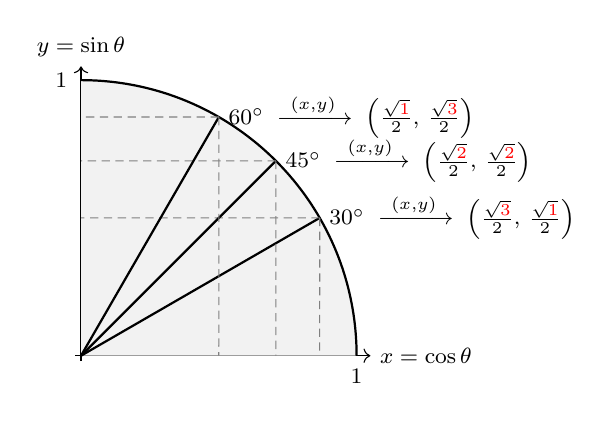
\begin{tikzpicture}[scale=3.5, font=\footnotesize]
  \tikzset{
    help/.style={densely dashed, thin, gray},
    pt/.style={circle, fill=black, inner sep=0.6pt}
  }

  % Assen
  \draw[->] (-0.02,0) -- (1.05,0) node[right] {$x=\cos\theta$};
  \draw[->] (0,-0.02) -- (0,1.05) node[above] {$y=\sin\theta$};

  % Eerste kwadrant boog
  \fill[gray!10] (0,0) -- (0:1) arc (0:90:1) -- cycle;
  \draw[thick] (0:1) arc (0:90:1);

  % Ticks bij 1
  \draw (1,0) -- ++(0,0.015) node[below=3pt] {$1$};
  \draw (0,1) -- ++(0.015,0) node[left=3pt] {$1$};

  % --- 30 graden ---
  \coordinate (P30) at (30:1);
  \draw[thick] (0,0) -- (P30);
  \draw[help] (P30) -- ({cos(30)},0);
  \draw[help] (P30) -- (0,{sin(30)});
  \fill[pt] (P30);
\node[anchor=west] at (30:1)
  {$30^\circ \;\xrightarrow[\text{ }]{\text{ }(x, y)\text{ }}\;
  \left(\tfrac{\sqrt{\textcolor{red}{3}}}{2},\,\tfrac{\sqrt{\textcolor{red}{1}}}{2}\right)$};
  
  % --- 45 graden ---
  \coordinate (P45) at (45:1);
  \draw[thick] (0,0) -- (P45);
  \draw[help] (P45) -- ({cos(45)},0);
  \draw[help] (P45) -- (0,{sin(45)});
  \fill[pt] (P45);
  \node[anchor=west] at (45:1) {$45^\circ \;\xrightarrow[\text{ }]{\text{ }(x, y)\text{ }}\;
\left(\tfrac{\sqrt{\textcolor{red}{2}}}{2},\,\tfrac{\sqrt{\textcolor{red}{2}}}{2}\right)$};

  % --- 60 graden ---
  \coordinate (P60) at (60:1);
  \draw[thick] (0,0) -- (P60);
  \draw[help] (P60) -- ({cos(60)},0);
  \draw[help] (P60) -- (0,{sin(60)});
  \fill[pt] (P60);
\node[anchor=west] at (60:1)
  {$60^\circ \;\xrightarrow[\text{ }]{\text{ }(x, y)\text{ }}\;
  \left(\tfrac{\sqrt{\textcolor{red}{1}}}{2},\,\tfrac{\sqrt{\textcolor{red}{3}}}{2}\right)$};
\end{tikzpicture}
\end{minipage}\hfill
\begin{minipage}[t]{0.35\linewidth}\vspace{0pt}
% --- Rechterzijde: Compacte tabel ---
\[
\begin{array}{c|cc}
\theta & \cos\theta & \sin\theta\\\hline
60^\circ & \tfrac{\sqrt{\textcolor{red}{1}}}{2} & \tfrac{\sqrt{\textcolor{red}{3}}}{2} \\[6pt]
45^\circ & \tfrac{\sqrt{\textcolor{red}{2}}}{2} & \tfrac{\sqrt{\textcolor{red}{2}}}{2} \\[6pt]
30^\circ & \tfrac{\sqrt{\textcolor{red}{3}}}{2} & \tfrac{\sqrt{\textcolor{red}{1}}}{2}
\end{array}
\]

\end{minipage}
\end{center}

\subsection{Radiaal}
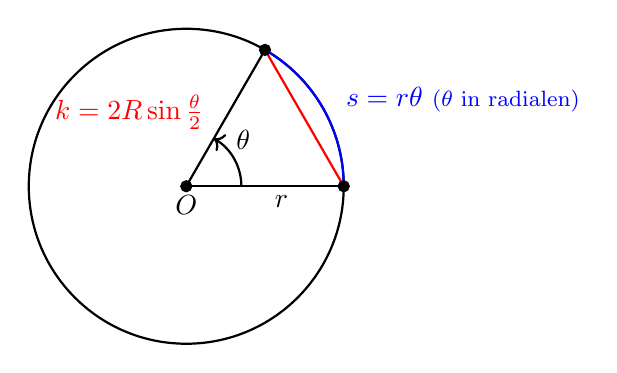
\begin{tikzpicture}

% Draw the circle
\draw[thick] (0,0) circle(2);

% Draw the radius lines
\draw[thick] (0,0) -- (60:2);
\draw[thick] (0,0) -- (0:2);
\draw[thick,red] (60:2) -- (0:2);

% Draw the arc
\draw[thick,blue] (0:2) arc[start angle=0, end angle=60, radius=2];

% Add the center point O
\filldraw[black] (0,0) circle(2pt) node[below] {\( O \)};

% Add the point on the arc
\filldraw[black] (60:2) circle(2pt);
\filldraw[black] (0:2) circle(2pt);

% Add labels
\node[below right] at (0:1) {\( r \)};
\node[right,blue] at (30:2.2) {\( s = r\theta \) \footnotesize (\(\theta\) in radialen)};
\node[left,red ] at (70:1) {$k = 2R \sin\frac{\theta}{2}$};
\node[above] at (25:0.8) {\( \theta \)};

% Draw the angle
\draw[thick,->] (0:0.7) arc[start angle=0, end angle=60, radius=0.7];

\end{tikzpicture}

\newpage

\subsection{Goniometrische formules}

\begin{table}[H]
\centering
\renewcommand{\arraystretch}{1.15}
\begin{tabular}{|m{0.52\textwidth}|m{0.43\textwidth}|}
\hline
% --- linkerkolom: formules in een minipage ---
\begin{minipage}[t]{\linewidth}\vspace{2pt}
\[
\begin{aligned}
\text{Sinusregel:}\quad 
& \frac{a}{\sin \alpha} 
= \frac{b}{\sin \beta} 
= \frac{c}{\sin \gamma} \\[6pt]
\text{Cosinusregel:}\quad
& \begin{cases}
a^{2} = b^{2} + c^{2} - 2bc \cos \alpha \\[6pt]
b^{2} = c^{2} + a^{2} - 2ca \cos \beta \\[6pt]
c^{2} = a^{2} + b^{2} - 2ab \cos \gamma
\end{cases}
\end{aligned}
\]
\end{minipage}
&
\begin{minipage}[t]{\linewidth}\centering\vspace{2pt}
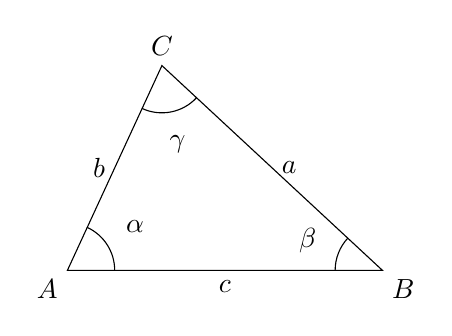
\begin{tikzpicture}[scale=1, line cap=round]
  % punten
  \coordinate (A) at (0,0);
  \coordinate (B) at (4,0);
  \coordinate (C) at (1.2,2.6);

  % driehoek
  \draw (A)--(B)--(C)--cycle;

  % hoeken BINNEN de driehoek
  \pic [draw, "$\alpha$", angle radius=6mm, angle eccentricity=1.7] {angle = B--A--C};
  \pic [draw, "$\beta$",  angle radius=6mm, angle eccentricity=1.7] {angle = C--B--A};
  \pic [draw, "$\gamma$", angle radius=6mm, angle eccentricity=1.7] {angle = A--C--B};

  % zijden
  \node[below] at ($(A)!0.5!(B)$) {$c$};
  \node[left]  at ($(A)!0.5!(C)$) {$b$};
  \node[right] at ($(B)!0.5!(C)$) {$a$};

  % hoekpunten
  \node[below left]  at (A) {$A$};
  \node[below right] at (B) {$B$};
  \node[above]       at (C) {$C$};
\end{tikzpicture}
\end{minipage}
\\ \hline
\end{tabular}
\end{table}

\[
\begin{array}{|l|l|}
\hline
{\scriptsize {Som-\;en\;verschilformules}} & 
{\scriptsize {Verdubbelingsformules}} \\ \hline
\sin(\alpha \pm \beta) = \sin\alpha \cos\beta \pm \cos\alpha \sin\beta \;\; \textcolor{blue}{\scriptsize (hetero's)} & 
\sin 2\alpha = 2\sin\alpha \cos\alpha \\ \hline
\cos(\alpha \pm \beta) = \cos\alpha \cos\beta \mp \sin\alpha \sin\beta \;\; \textcolor{blue}{\scriptsize (homo's)} & 
\begin{aligned}
\cos 2\alpha &= \cos^2\alpha - \sin^2\alpha \\[4pt]
             &= 1 - 2\sin^2\alpha \quad \textcolor{blue}{\scriptsize (*)} \\[4pt]
             &= 2\cos^2\alpha - 1 \quad \textcolor{blue}{\scriptsize (**)}
\end{aligned} \\ \hline
\tan(\alpha \pm \beta) = \dfrac{\tan\alpha \pm \tan\beta}{1 \mp \tan\alpha \tan\beta} & 
\tan 2\alpha = \dfrac{2\tan\alpha}{1 - \tan^2\alpha} \\ \hline
\end{array}
\]


\[
\begin{array}{|l|l|l|}
\hline
\sin^2\alpha = \dfrac{1 - \cos 2\alpha}{2} \quad (*) & 
\parbox{3.5cm}{\centering Verdubbelingsformules \\ $f(\tan\alpha)$} & 
t-formules, \quad \tan\dfrac{\alpha}{2} = t \\ \hline

\cos^2\alpha = \dfrac{1 + \cos 2\alpha}{2} \quad (**) & 
\sin 2\alpha = \dfrac{2\tan\alpha}{1 + \tan^2\alpha} & 
\sin\alpha = \dfrac{2t}{1 + t^2} \\ \hline

Halveringsformules & 
\cos 2\alpha = \dfrac{1 - \tan^2\alpha}{1 + \tan^2\alpha} & 
\cos\alpha = \dfrac{1 - t^2}{1 + t^2} \\ \hline

\sin\dfrac{\alpha}{2} = \pm\sqrt{\dfrac{1 - \cos\alpha}{2}} & 
\tan 2\alpha = \dfrac{2\tan\alpha}{1 - \tan^2\alpha} & 
\tan\alpha = \dfrac{2t}{1 - t^2} \\ \hline

\cos\dfrac{\alpha}{2} = \pm\sqrt{\dfrac{1 + \cos\alpha}{2}} & & \\ \hline
\end{array}
\]
\[
\begin{array}{|c|c|}
\hline
& \text{Omgekeerde formules van Simpson} \\ \hline

\sin(\alpha \pm \beta) = \sin\alpha\cos\beta \pm \cos\alpha\sin\beta &
\sin(\alpha + \beta) + \sin(\alpha - \beta) = 2\sin\alpha\cos\beta \\

& \sin(\alpha + \beta) - \sin(\alpha - \beta) = 2\cos\alpha\sin\beta \\ \hline

\cos(\alpha \pm \beta) = \cos\alpha\cos\beta \mp \sin\alpha\sin\beta &
\cos(\alpha + \beta) + \cos(\alpha - \beta) = 2\cos\alpha\cos\beta \\

& \cos(\alpha + \beta) - \cos(\alpha - \beta) = -2\sin\alpha\sin\beta \\ \hline

\end{array}
\]
\[
\begin{array}{|c|c|}
\hline
\multicolumn{2}{|c|}{\text{Formules van Simpson}} \\ \hline
\begin{aligned}
\sin \alpha + \sin \beta &= 2\sin\left(\frac{\alpha + \beta}{2}\right)\cos\left(\frac{\alpha - \beta}{2}\right) \\
\sin \alpha - \sin \beta &= 2\cos\left(\frac{\alpha + \beta}{2}\right)\sin\left(\frac{\alpha - \beta}{2}\right)
\end{aligned} & 
\begin{aligned}
\cos \alpha + \cos \beta &= 2\cos\left(\frac{\alpha + \beta}{2}\right)\cos\left(\frac{\alpha - \beta}{2}\right) \\
\cos \alpha - \cos \beta &= -2\sin\left(\frac{\alpha + \beta}{2}\right)\sin\left(\frac{\alpha - \beta}{2}\right)
\end{aligned} \\
\hline
\end{array}
\]
\newpage

\subsection{Cyclometrische formules}

% — Definities ---------------------------------------------------------------
\[
\begin{aligned}
y=Bgsin x &\;\Leftrightarrow\; x=\sin y,  && \text{met } y\in\left[-\tfrac{\pi}{2},\tfrac{\pi}{2}\right],\ x\in[-1,1]\\
y=Bgcos x &\;\Leftrightarrow\; x=\cos y,  && \text{met } y\in[0,\pi],\ x\in[-1,1]\\
y=Bgtan x &\;\Leftrightarrow\; x=\tan y,  && \text{met } y\in\left]-\tfrac{\pi}{2},\tfrac{\pi}{2}\right[,\ x\in\mathbb{R}\\
y=Bgcot x &\;\Leftrightarrow\; x=\cot y,  && \text{met } y\in\left]0,{\pi}\right[,\ x\in\mathbb{R}
\end{aligned}
\]

\[
\begin{aligned}
&\forall a \in \mathbb{R}_0^+ : && Bgcot(a) = Bgtan\!\left(\frac{1}{a}\right) \\
&\forall a \in \mathbb{R}_0^- : && Bgcot(a) = \pi + Bgtan\!\left(\frac{1}{a}\right)
\end{aligned}
\]



% — Figuur -------------------------------------------------------------------
% Vereist: \usepackage{tikz,pgfplots}
% \pgfplotsset{compat=1.18}
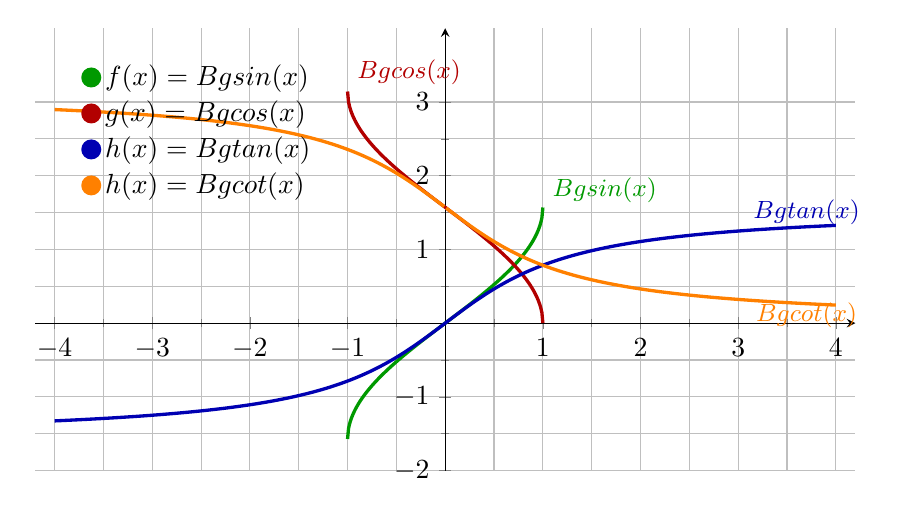
\begin{tikzpicture}
\begin{axis}[
  width=12cm,height=7.2cm,
  axis lines=middle,
  xmin=-4.2,xmax=4.2,
  ymin=-2,ymax=4,
  grid=both, minor tick num=1,
  xtick={-4,-3,-2,-1,0,1,2,3,4},
  ytick={-2,-1,0,1,2,3},
  clip=false,
  trig format=rad,             % functies in radialen
  every axis plot/.style={very thick},
  legend style={
    draw=none, fill=none,
    legend columns=1,
    at={(axis cs:-3.8,2.6)},
    anchor=west
  },
  legend image code/.code={\draw[mark=*,mark size=3pt] plot coordinates {(0,0)};},
  legend cell align=left
]

% f(x) = asin(x)
\addplot[green!60!black,domain=-1:1,samples=200] {asin(x)};
\addlegendentry{$f(x)=Bgsin(x)$}

% g(x) = acos(x)
\addplot[red!70!black,domain=-1:1,samples=200] {acos(x)};
\addlegendentry{$g(x)=Bgcos(x)$}

% h(x) = atan(x)
\addplot[blue!70!black,domain=-4:4,samples=200] {atan(x)};
\addlegendentry{$h(x)=Bgtan(x)$}

% i(x) = acot(x)
\addplot[orange,domain=-4:-0.01,samples=200] {pi+atan(1/x)};
\addplot[orange,domain=0.01:4,samples=200] {atan(1/x)};
\addlegendentry{$h(x)=Bgcot(x)$}

% labels bij de krommen
\node[green!60!black,anchor=south west] at (axis cs:1,1.5)  {\small $Bgsin(x)$};
\node[red!70!black,anchor=south west]   at (axis cs:-1,3.1) {\small $Bgcos(x)$};
\node[blue!70!black]  at (axis cs:3.7,1.5)  {\small $Bgtan(x)$};
\node[orange]         at (axis cs:3.7,0.1)   {\small $Bgcot(x)$};

\end{axis}
\end{tikzpicture}

% — Identiteiten 
\begin{tabular}{|p{0.45\textwidth}|p{0.45\textwidth}|} % 2 columns
  \hline
    \begin{minipage}{0.45\linewidth}
    \makebox[\linewidth][l]{%
      $\begin{aligned}
      &\sin\bigl(Bgsin(x)\bigr) = x, \; x \in [-1,1] \\
      &\cos\bigl(Bgcos(x)\bigr) = x, \; x \in [-1,1] \\
      &\tan\bigl(Bgtan(x)\bigr) = x, \; x \in\mathbb{R}\\
      &\cot\bigl(Bgcot(x)\bigr) = x, \; x \in\mathbb{R}\\
    	  &\end{aligned}$%
    }
    \end{minipage}
    &
    \begin{minipage}{0.45\linewidth}
    \makebox[\linewidth][l]{%
      $\begin{aligned}
  	  &Bgsin(\sin(x)) = x, -\frac{\pi}{2} \le x \le \frac{\pi}{2} \\
      &Bgcos(\cos(x)) = x, 0 \le x \le \pi \\
      &Bgtan(\tan(x)) = x, -\frac{\pi}{2} < x < \frac{\pi}{2} \\
      &Bgcot(\cot(x)) = x, 0 < x < \pi
    	  &\end{aligned}$%
    	}
    \end{minipage}
    \\
    \hline
    \begin{minipage}{0.45\linewidth}
    \makebox[\linewidth][l]{%
	  $\begin{aligned}
	  &\cos(bgsin(x)) = \sqrt{1 - x^2}, \; x \in [-1,1] \\
	  &\sin(bgcos(x)) = \sqrt{1 - x^2}, \; x \in [-1,1] \\
	  &\cot(bgtan(x)) = \frac{1}{x}, \; \forall x \in \mathbb{R}_0 \\
	  &\tan(bgcot(x)) = \frac{1}{x}, \; \forall x \in \mathbb{R}_0 \\
	  &\cos\bigl(Bgtan(x)\bigr) = \dfrac{1}{\sqrt{1+x^2}}, \; x\in\mathbb{R}\\
	  &\sin\bigl(Bgtan(x)\bigr) = \dfrac{x}{\sqrt{1+x^2}}, \; x\in\mathbb{R}\\
	  &\end{aligned}$%
    	}
    \end{minipage}
    &
    \begin{minipage}{0.45\linewidth}
    \makebox[\linewidth][l]{%
      $\begin{aligned}
      &Bgsin(-x) = -\,Bgsin(x) , \; x\in[-1,1]\\
      &Bgcos(-x) = \pi-Bgcos(x) , \; x\in[-1,1]\\
      &Bgsin(x) + Bgcos(x) = \dfrac{\pi}{2} , \; x\in[-1,1]\\
      &Bgcot(x) + Bgtan(x) = \dfrac{\pi}{2} , \; x\in\mathbb{R}
    	  &\end{aligned}$%
    	}
    \end{minipage}
    \\
    \hline
\end{tabular}

\newpage

% --- Section: Exponentiële en logaritmische functies -------------------------------------------------------
\section{Exponentiële en logaritmische functies}
\begin{tabular}{|p{0.46\linewidth}|p{0.46\linewidth}|}
\hline
% ======= TOP LEFT =======
\begin{minipage}[t]{\linewidth}\raggedright
\[
\begin{aligned}
&{}^a\!\log x = y \Leftrightarrow x=a^y, (x>0,a>0,a\neq 1)\\
&{}^a\log {a^y} = y\; \Leftrightarrow x = {a^{{}^a\log x}}\\
&{}^a\!\log(x_1x_2)={}^a\!\log x_1+{}^a\!\log x_2\\
&{}^a\!\log\!\left(\frac{x_1}{x_2}\right)={}^a\!\log x_1-{}^a\!\log x_2\\
&{}^a\!\log\!\left(\frac1x\right)=-\,{}^a\!\log x\\
&{}^a\!\log(x^n)=n\,{}^a\!\log x\\
&{}^b\!\log x=\frac{{}^a\!\log x}{{}^a\!\log b}\\
&{}^b\!\log a=\frac1{{}^a\!\log b}
\end{aligned}
\]
\end{minipage}
&
% ======= TOP RIGHT =======
\begin{minipage}[t]{\linewidth}\raggedright
\[
\begin{aligned}
&e=\lim_{x\to\pm\infty}\left(1+\frac{1}{x}\right)^{x}=\lim_{h\to0}(1+h)^{1/h}\\
&e\approx 2{,}718\dots\\
&\text{(L'H\^opital) }\left(\frac{0}{0},\frac{\pm\infty}{\pm\infty}\right) \\
&\displaystyle \lim_{x\to a}\frac{f(x)}{g(x)}=\lim_{x\to a}\frac{f'(x)}{g'(x)}\\
&e=1+\frac{1}{1!}+\frac{1}{2!}+\frac{1}{3!}+\cdots \\
&\frac{{e - 1}}{2} = \frac{1}{{1 + \frac{1}{{6 + \frac{1}{{10 + \frac{1}{{14 + \frac{1}{{18 +  + \frac{{...}}{{...}}}}}}}}}}}} \\
&e - 1 = 1 + \frac{1}{{1 + \frac{1}{{2 + \frac{1}{{1 + \frac{1}{{1 + \frac{1}{{4 + \frac{1}{{1 + \frac{1}{{1 + \frac{1}{{6 + \frac{1}{{1 + }}}}}}}}}}}}}}}}}}
\end{aligned}
\]
\end{minipage}
\\ \hline
% ======= BOTTOM LEFT =======
\begin{minipage}[t]{\linewidth}\centering
\textbf{\(a>1\)}\\[1mm]
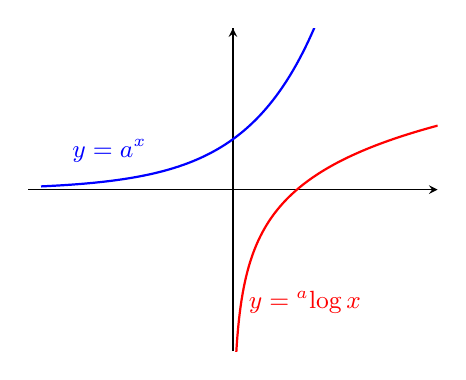
\begin{tikzpicture}
\begin{axis}[
  width=5.2cm, height=4.1cm, scale only axis,
  xmin=-3.2, xmax=3.2, ymin=-3.2, ymax=3.2,
  axis lines=middle, xtick=\empty, ytick=\empty,
  clip=true, enlarge x limits=false, enlarge y limits=false,
  trim axis left, trim axis right
]
  \def\a{2.5}
  % Exponential (blue)
  \addplot[smooth, domain=-3:3, samples=200, thick, blue] {(\a^x)} node[pos=0.1, above left, blue] {\small $y=a^x$};
  % Logarithmic (red)
  \addplot[smooth, domain=0.05:3.2, samples=200, thick, red] {ln(x)/ln(\a)} node[pos=0.1, above right, red] {\small $y={}^a\!\log x$};
  % Dashed axis line
  \addplot[dashed] coordinates {(0,-3.2) (0,3.2)};
\end{axis}
\end{tikzpicture}

\[
\begin{aligned}
&\lim_{x\to-\infty}a^x=0 \\
&\lim_{x\to+\infty}a^x=+\infty \\
&\lim_{x\to0^+}{}^a\!\log x=-\infty \\
&\lim_{x\to+\infty}{}^a\!\log x=+\infty \\
&
\end{aligned}
\]
\end{minipage}
&
% ======= BOTTOM RIGHT =======
\begin{minipage}[t]{\linewidth}\centering
\textbf{\(0<a<1\)}\\[1mm]
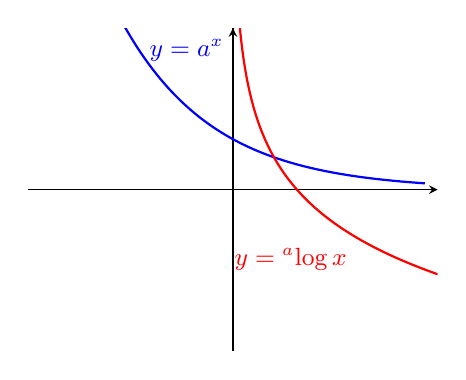
\begin{tikzpicture}
\begin{axis}[
  width=5.2cm, height=4.1cm, scale only axis,
  xmin=-3.2, xmax=3.2, ymin=-3.2, ymax=3.2,
  axis lines=middle, xtick=\empty, ytick=\empty,
  clip=true, enlarge x limits=false, enlarge y limits=false,
  trim axis left, trim axis right
]
  \def\a{0.5}
  % Exponential (blue)
  \addplot[smooth, domain=-3:3, samples=200, thick, blue] {(\a^x)} node[pos=0.5, right, blue] {\small $y=a^x$};
  % Logarithmic (red)
  \addplot[smooth, domain=0.05:3.2, samples=200, thick, red] {ln(x)/ln(\a)} node[pos=0.8, below left, red] {\small $y={}^a\!\log x$};
  % Dashed axis line
  \addplot[dashed] coordinates {(0,-3.2) (0,3.2)};
\end{axis}
\end{tikzpicture}

\[
\begin{aligned}
&\lim_{x\to-\infty}a^x=+\infty \\
&\lim_{x\to+\infty}a^x=0 \\
&\lim_{x\to0^+}{}^a\!\log x=+\infty \\
&\lim_{x\to+\infty}{}^a\!\log x=-\infty \\
&
\end{aligned}
\]
\end{minipage}
\\ \hline
\end{tabular}

\newpage
% --- Section: Matrices -------------------------------------------------------
\section{Matrices}
\subsection{Symbolen}

\begingroup
\renewcommand{\arraystretch}{1.2}
\begin{tabular}{ll}
$A$        & matrix $A$ \\
$a_{ij}$   & het element op rij $i$ en in kolom $j$ \\
$A_{ij}$   & cofactor van het element op rij $i$ en in kolom $j$ \\
$I$        & de eenheidsmatrix \\
$A^{-1}$   & de inverse matrix \\
$A^{T}$    & de getransponeerde matrix \\
$\det A$   & determinant van de vierkante matrix $A$
\end{tabular}
\endgroup
% ----------------------------------------------------------------------------- 


% --- Section: Matrix Rekenregels ---------------------------------------------
\subsection{Rekenregels}

\textbf{Opgelet:} onderstaande regels gelden enkel onder de juiste voorwaarden.

\begin{center}
\renewcommand{\arraystretch}{1.4}
\begin{tabular}{>{$}l<{$} l}
A + B = B + A & commutativiteit van de optelling \\
A + (B + C) = (A + B) + C & associativiteit van de optelling \\
A \cdot I = A = I \cdot A & eenheidsmatrix \\
A(BC) = (AB)C & associativiteit van de vermenigvuldiging \\
A(B + C) = AB + AC & linker distributiviteit \\
(B + C)A = BA + CA & rechter distributiviteit \\
AB \neq BA & niet-commutatief in het algemeen \\
(A + B)^T = A^T + B^T &  \\
(cA)^T = cA^T &  \\
(AC)^T = C^T A^T &  \\
(A^T)^T = A &  \\
I^T = I &  \\
A \cdot A^{-1} = I = A^{-1} \cdot A &  \\
(AB)^{-1} = B^{-1} A^{-1} &  \\
B = C \;\Rightarrow\; AB = AC \;\;\text{en}\;\; BA = CA & $A$ regulier
\end{tabular}
\end{center} 

% --- TikZ: tekenpatroon (-1)^{i+j} -------------------------------------------
\subsection{Cofactor-tekenpatroon \texorpdfstring{$(-1)^{i+j}$}{(-1)^{i+j}}}

\begin{center}
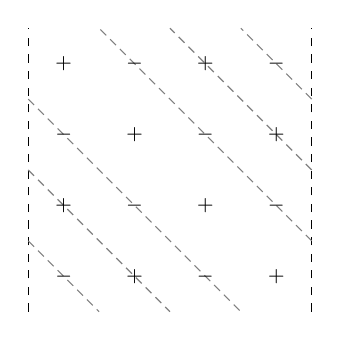
\begin{tikzpicture}[scale=1, every node/.style={font=\scriptsize}]
  \def\n{4}      % grootte n x n
  \def\cell{0.9} % celgrootte

  % buitenste haakjes [   ]
  \draw[thin,dashed] (0,0) -- (0,\n*\cell);
  \draw[thin,dashed] (\n*\cell,0) -- (\n*\cell,\n*\cell);

  % gestippelde diagonalen (familie met helling -1)
  \foreach \m in {1,...,\numexpr\n-1\relax}{
    \draw[densely dashed, gray] (0,\m*\cell) -- (\m*\cell,0);
    \draw[densely dashed, gray] (\n*\cell,\m*\cell) -- (\m*\cell,\n*\cell);
  }

  % plus/minus in de cencentra
  \foreach \i in {1,...,\n}{
    \foreach \j in {1,...,\n}{
      \pgfmathtruncatemacro{\parity}{mod(\i+\j,2)}
      \pgfmathsetmacro{\x}{(\j-0.5)*\cell}
      \pgfmathsetmacro{\y}{\n*\cell - (\i-0.5)*\cell}
      \ifnum\parity=0
        \node at (\x,\y) {$+$};
      \else
        \node at (\x,\y) {$-$};
      \fi
    }
  }
\end{tikzpicture}
\end{center}

% ----------------------------------------------------------------------------- 
% --- Determinanten (2x groter diagram, beide methodes in kolom) --------------
\section{Determinanten}

\begin{center}
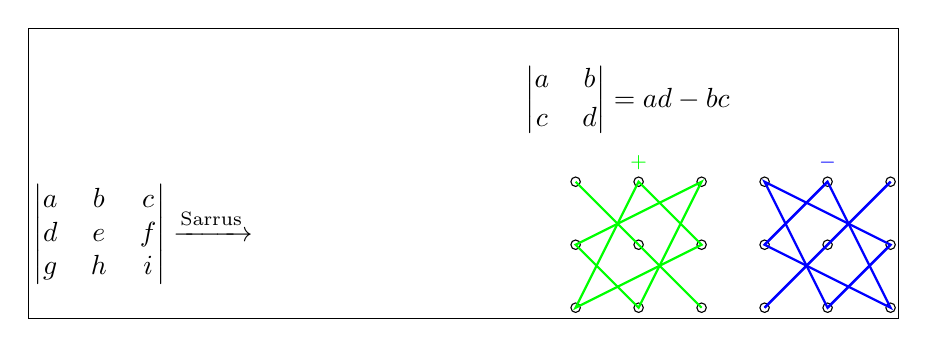
\begin{tikzpicture}[>=stealth]
\node (box1) [draw, inner sep=2pt, minimum width=10cm, align=center] at (0,0) {%
  \begin{minipage}{0.9\linewidth}
  \[
  \setlength{\arraycolsep}{6pt}%
  \begin{matrix}
    % --- 2x2 determinant ---------------------------------------------------
    \displaystyle
    \left|\begin{matrix} a & b \\[2pt] c & d \end{matrix}\right|
    = ad - bc
    \\[1.2em]
    % --- 3x3 determinant (Sarrus) -----------------------------------------
    \displaystyle
    \left|\begin{matrix} a & b & c \\ d & e & f \\ g & h & i \end{matrix}\right|
    \mathrel{\smash{\xrightarrow{\scriptsize\text{Sarrus}}}}%
    \mkern-10mu
    \tikz[scale=2, baseline=-5ex, xshift=-3cm]{%
      \def\cell{0.40}
      \tikzset{
        triPlus/.style={thick,green},
        triMinus/.style={thick,blue}
      }

      % -------- PLUS (links) ----------
      \begin{scope}[shift={(0,0)}]
        % grid
        \foreach \i in {0,1,2}{
          \foreach \j in {0,1,2}{
            \draw (\j*\cell,-\i*\cell) circle(0.03);
          }
        }
        \node[above=2pt, text=green] at (\cell,0) {\scriptsize $\mathbf{+}$};
        \draw[triPlus] (0,0) -- (\cell,-\cell) -- (2*\cell,-2*\cell);
        \draw[triPlus] (1*\cell,0) -- (2*\cell,-1*\cell) -- (0,-2*\cell) -- cycle;
        \draw[triPlus] (2*\cell,0) -- (0,-1*\cell) -- (1*\cell,-2*\cell) -- cycle;
      \end{scope}

      % -------- MIN (rechts) ----------
      \begin{scope}[shift={(1.2,0)}]
        % grid
        \foreach \i in {0,1,2}{
          \foreach \j in {0,1,2}{
            \draw (\j*\cell,-\i*\cell) circle(0.03);
          }
        }
        \node[above=2pt, text=blue] at (\cell,0) {\scriptsize $\mathbf{-}$};
        \draw[triMinus] (0,-2*\cell) -- (\cell,-1*\cell) -- (2*\cell,0);
        \draw[triMinus] (0,-1*\cell) -- (\cell,0);
        \draw[triMinus] (\cell,-2*\cell) -- (2*\cell,-1*\cell);
        \draw[triMinus] (2*\cell,0) -- (1*\cell,-1*\cell) -- (0,-2*\cell) -- cycle;
        \draw[triMinus] (1*\cell,0) -- (0,-1*\cell) -- (2*\cell,-2*\cell) -- cycle;
        \draw[triMinus] (0,0) -- (2*\cell,-1*\cell) -- (1*\cell,-2*\cell) -- cycle;
      \end{scope}
    }
  \end{matrix}
  \]
  \end{minipage}%
};
\end{tikzpicture}
\end{center}



% -----------------------------------------------------------------------------
% --- Section: Stelsels oplossen ----------------------------------------------
\newpage

\section{Stelsels oplossen}

\subsection{Rang van een matrix}
$ \operatorname{rang}(A) = \text{het aantal lineair onafhankelijke rijen van } A $

\begin{enumerate}
  \item Breng de matrix in \textbf{gereduceerde rij-echelonvorm \scriptsize \\ (RREF=Reduced Row-Echelon Form)}.
  
  \item Het aantal niet-nulrijen in deze trapvorm is de rang van \(A\).
\end{enumerate}

\subsection{n vergelijkingen met n onbekenden, $|A|\neq 0$ (Cramer)}
Voor $AX=B$ met $A\in\mathbb{R}^{n\times n}$ en $\det(A)\neq0$ geldt
\[
x_j = \frac{\det(A_j)}{\det(A)} \qquad (j=1,\dots,n),
\]
waar $A_j$ ontstaat uit $A$ door de $j$-de kolom te vervangen door de vector $B$.

\subsection{Homogene $2\times 3$-stelsels}
\begin{align*}
a_1 x + b_1 y + c_1 z &= 0, \\
a_2 x + b_2 y + c_2 z &= 0.
\end{align*}
Indien $\det\!\begin{pmatrix} a_1 & b_1 \\ a_2 & b_2 \end{pmatrix}\neq0$, dan is de oplossingenverzameling
\[
V = \{\, \lambda \cdot (\det\!\begin{pmatrix} b_1 & c_1 \\ b_2 & c_2 \end{pmatrix}, \;
          -\det\!\begin{pmatrix} a_1 & c_1 \\ a_2 & c_2 \end{pmatrix}, \;
           \det\!\begin{pmatrix} a_1 & b_1 \\ a_2 & b_2 \end{pmatrix}) \mid \lambda\in\mathbb{R}\,\}.
\]

\subsection{$n+1$ vergelijkingen met $n$ onbekenden}
Een stelsel van de vorm
\begin{align*}
a_1 x + b_1 y + c_1 &= 0,\\
a_2 x + b_2 y + c_2 &= 0,\\
a_3 x + b_3 y + c_3 &= 0
\end{align*}
heeft één oplossing $\Leftrightarrow$
\[
\det \begin{pmatrix}
a_1 & b_1 & c_1 \\
a_2 & b_2 & c_2 \\
a_3 & b_3 & c_3
\end{pmatrix}=0.
\]

% -----------------------------------------------------------------------------


\section{Meetkunde}

$
\begin{array}{|l|l|}
\hline
\text{Afstand 2 punten} & \left| {{P_1}({x_1},{y_1}),{P_2}({x_2},{y_2})} \right| = \sqrt {{{({x_2} - {x_1})}^2} + {{({y_2} - {y_1})}^2}}  \\
 & \begin{array}{l}
\left| {{P_1}({x_1},{y_1},{z_1}),{P_2}({x_2},{y_2},{z_2})} \right| = \\
\sqrt {{{({x_2} - {x_1})}^2} + {{({y_2} - {y_1})}^2} + {{({z_2} - {z_1})}^2}} 
\end{array} \\
\hline
\text{Midden v/e lijnstuk} & co(M) = (\frac{{({x_1} + {x_2})}}{2},\frac{{({y_1} + {y_2})}}{2})\\
\hline
\text{Zwaartepunt v/e driehoek} & co(Z) = (\frac{{({x_1} + {x_2} + {x_3})}}{3},\frac{{({y_1} + {y_2} + {y_3})}}{3})\\
\hline
\end{array}
$
\newline
$
\begin{array}{|l|l|}
\hline
\text{Vergelijking v/e rechte dr punt met rico m} & y - {y_1} = m(x - {x_1})  \\
\hline
\text{Vergelijking v/e rechte dr punt met rico m} & y - {y_1} = \frac{{{y_2} - {y_1}}}{{{x_2} - {x_1}}}(x - {x_1})  \\
\hline
\text{Vergelijking v/e rechte dr snijpunt met x-as (r,0) en y-as (0,s)} & \frac{x}{r} + \frac{y}{s} = 1  \\
\hline
\text{Hoek tussen twee rechten a,b met rico m1,m2} & \cos (\widehat {ab}) = \frac{{\left| {1 + {m_1}{m_2}} \right|}}{{\sqrt {1 + {m_1}^2} \sqrt {1 + {m_2}^2} }}  \\
\hline
\text{Afstand tussen rechte a $\leftrightarrow$ ux+vy+w=0 en P(x1,y1)} & d(P,a) = \frac{{\left| {u{x_1} + v{y_1} + w} \right|}}{{\sqrt {{u^2} + {v^2}} }}  \\
\hline
\end{array}
$

\subsection{De cirkel}

$
\begin{array}{|l|l|}
\hline
\text{Cartesiaanse vergelijking} & {(x - {x_1})^2} + {(y - {y_1})^2} = {r^2}  \\
\hline
\text{Algemene vergelijking} & {x^2} + {y^2} + 2ax + 2by + c = 0\quad  \wedge \quad {a^2} + {b^2} - c \ge 0  \\
\hline
\text{Parameter vergelijking} & \left\{ {\begin{array}{*{20}{c}}
{x = {x_M} + r.\cos t}\\
{y = {y_M} + r.\sin t}
\end{array}} \right.\;\quad \quad met\;t \in \left[ {0,2\pi } \right[  \\
\hline
\end{array}
$

\subsection{De parabool}

$
\begin{array}{|l|l|}
\hline
\text{Top vergelijking} & {y^2} = 2px  \\
\hline
\text{Parameter vergelijking} & \begin{array}{l}
x = 2p{\lambda ^2}\quad \quad met\;\lambda  \in \mathbb {R} \\
y = 2p\lambda 
\end{array}  \\
\hline
\end{array}
$
\subsection{De ellips}
\vspace{-3mm}
\begin{table}[h!]
    \begin{tabular}{|>{\centering\arraybackslash}m{0.4\textwidth}|>{\centering\arraybackslash}m{0.55\textwidth}|}
        \hline
        \[\begin{array}{l}
Cartesiaanse{\rm{ }}vgl.{\rm{ }}:\frac{{{x^2}}}{{{a^2}}} + {\frac{y}{{{b^2}}}^2} = 1\\
Parameter{\rm{ }}vgl.{\rm{ }}:\\
\left\{ {\begin{array}{*{20}{c}}
{x = a.\cos t}\\
{y = b.\sin t}
\end{array}} \right.\;\quad \quad met\;t \in \left[ {0,2\pi } \right[
\end{array}\]
        &
        \vspace{2mm}
        \begin{minipage}[t]{0.55\textwidth}
			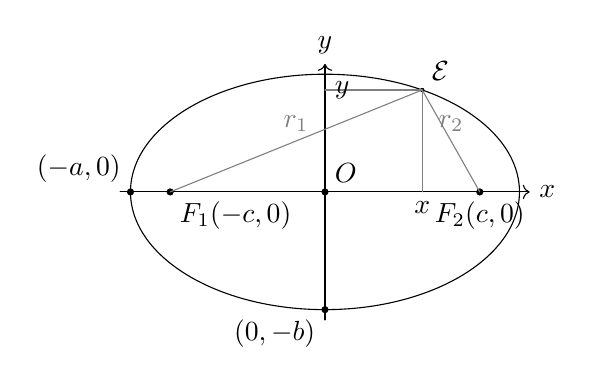
\begin{tikzpicture}[scale=0.65, line cap=round]
			  % Parameters
			  \pgfmathsetmacro{\a}{3.8}
			  \pgfmathsetmacro{\b}{2.3}
			  \pgfmathsetmacro{\c}{sqrt(max(\a*\a-\b*\b,0))} % c^2 = a^2 - b^2 (ellipse)
			
			  % Axes
			  \draw[->] (-4,0) -- (4,0) node[right] {$x$};
			  \draw[->] (0,-2.5) -- (0,2.5) node[above] {$y$};
			
			  % Ellipse
			  \draw (0,0) ellipse [x radius=\a, y radius=\b];
			
			  % Foci and key points
			  \fill (-\c,0) circle (2pt) node[below right] {$F_1(-c,0)$};
			  \fill (\c,0)  circle (2pt) node[below ] {$F_2(c,0)$};
			  \fill (0,0)   circle (2pt) node[above right] {$O$};
			  \fill (-\a,0) circle (2pt) node[above left] {$(-a,0)$};
			  \fill (0,-\b) circle (2pt) node[below left] {$(0,-b)$};
			
			  % Point P on ellipse (parametric angle t)
			  \pgfmathsetmacro{\t}{60} % degrees
			  \pgfmathsetmacro{\xP}{ \a*cos(\t) }
			  \pgfmathsetmacro{\yP}{ \b*sin(\t) }
			  \fill (\xP,\yP) circle (1.2pt) node[above right] {$\mathcal{E}$};
			
			  % r1 and r2
			  \draw[gray] (\xP,\yP) -- (-\c,0) node[midway, above] {$r_1$};
			  \draw[gray] (\xP,\yP) -- (\c,0)  node[midway, above] {$r_2$};
			
			  % Projections to axes (x and y)
			  \draw[gray] (\xP,\yP) -- (\xP,0);   % vertical drop
			  \draw[gray] (\xP,\yP) -- (0,\yP);   % horizontal to y-axis
			  \node[below] at (\xP,0) {$x$};
			  \node[right] at (0,\yP) {$y$};
			\end{tikzpicture}

        \end{minipage} \\ 
        \hline
    \end{tabular}
\end{table}

\newpage

\subsection{De hyperbool}

\vspace{-3mm}
\begin{table}[h!]
    \begin{tabular}{|>{\centering\arraybackslash}m{0.5\textwidth}|>{\centering\arraybackslash}m{0.45\textwidth}|}
        \hline
        \[\begin{array}{l}
Cartesiaanse{\rm{ }}vgl.{\rm{ }}:\frac{{{x^2}}}{{{a^2}}} - {\frac{y}{{{b^2}}}^2} = 1\\
Parameter{\rm{ }}vgl.{\rm{ }}:\\
\left\{ {\begin{array}{*{20}{c}}
{x = a.\sec t}\\
{y = b.\tan t}
\end{array}} \right.\;\quad \quad met\;t \in \left] {\frac{{ - \pi }}{2},\frac{{3\pi }}{2}} \right[\backslash \left\{ {\frac{\pi }{2}} \right\}
\end{array}\]
        &
        \vspace{2mm}
        \begin{minipage}[t]{0.45\textwidth}
		 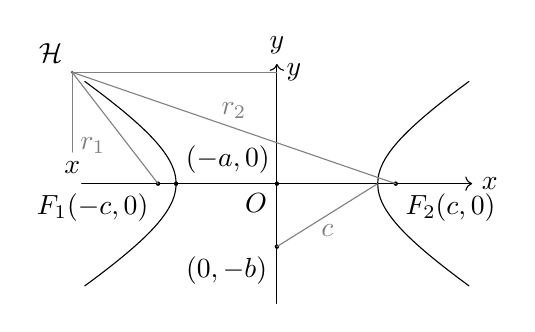
\begin{tikzpicture}[scale=0.4, line cap=round]
		  % Parameters
		  \pgfmathsetmacro{\a}{3.2}
		  \pgfmathsetmacro{\b}{2.0}
		  \pgfmathsetmacro{\c}{sqrt(\a*\a+\b*\b)}  % c^2 = a^2 + b^2 (hyperbola)
		
		  % Axes
		  \draw[->] (-6.2,0) -- (6.2,0) node[right] {$x$};
		  \draw[->] (0,-3.8) -- (0,3.8) node[above] {$y$};
		
		  % Hyperbola branches: y = ± b*sqrt(x^2/a^2 - 1)
		  \draw[domain=\a:6.1,samples=150,smooth] plot (\x,  { \b*sqrt(\x*\x/(\a*\a) - 1) });
		  \draw[domain=\a:6.1,samples=150,smooth] plot (\x, -{ \b*sqrt(\x*\x/(\a*\a) - 1) });
		  \draw[domain=-6.1:-\a,samples=150,smooth] plot (\x,  { \b*sqrt(\x*\x/(\a*\a) - 1) });
		  \draw[domain=-6.1:-\a,samples=150,smooth] plot (\x, -{ \b*sqrt(\x*\x/(\a*\a) - 1) });
		
		  % Foci and key points
		  \fill (-\c,0) circle (2pt) node[below left] {$F_1(-c,0)$};
		  \fill (\c,0)  circle (2pt) node[below right] {$F_2(c,0)$};
		  \fill (0,0)   circle (2pt) node[below left] {$O$};
		  \fill (-\a,0) circle (2pt) node[above right] {$(-a,0)$};
		  \fill (0,-\b) circle (2pt) node[below left] {$(0,-b)$};
		
		  % Choose a point P on the left-upper branch
		  \pgfmathsetmacro{\xP}{-6.5}
		  \pgfmathsetmacro{\yP}{ \b*sqrt(\xP*\xP/(\a*\a) - 1) }
		  \fill (\xP,\yP) circle (1.2pt) node[above left] {$\mathcal{H}$};
		
		  % r1 and r2
		  \draw[gray] (\xP,\yP) -- (-\c,0) node[midway, below left] {$r_1$};
		  \draw[gray] (\xP,\yP) -- (\c,0)  node[midway, above] {$r_2$};
		
		  % Projections to axes (x and y)
		  \draw[gray] (\xP,\yP) -- (\xP,1);             % vertical drop
		  \draw[gray] (\xP,\yP) -- (0,\yP);             % horizontal to y-axis
		  \draw[gray] (0,-\b) -- (\a,0)    node[midway, below] {$c$};
		  \node[above] at (\xP,0) {$x$};
		  \node[right] at (0,\yP) {$y$};
		\end{tikzpicture}

        \end{minipage} \\ 
        \hline
    \end{tabular}
\end{table}

\subsection{Oppervlakte Formules}

\begin{table}[h!]
\begin{tabular}{|l|l|l|}
\hline
\textbf{Vorm} & \textbf{Formule} & \textbf{Variabelen} \\
\hline
Vierkant & $A = s^2$ & $s$: zijlengte \\
\hline
Rechthoek & $A = l.w$ & $l$: lengte, $w$: breedte \\
\hline
Driehoek & $A = \frac{1}{2} b.h$ & $b$: basis, $h$: hoogte \\
\hline
Cirkel & $A = \pi r^2$ & $r$: straal \\
\hline
Parallellogram & $A = b.h$ & $b$: basis, $h$: hoogte \\
\hline
Trapezium & $A = \frac{1}{2} (b_1 + b_2).h$ & $b_1, b_2$: bases, $h$: hoogte \\
\hline
Ellips & $A = \pi a.b$ & $a, b$: halve grote en halve kleine as \\
\hline
Regelmatig Veelhoek & $A = \frac{1}{2} P.a$ & $P$: omtrek, $a$: apothema \\
\hline
\end{tabular}
\end{table}

\subsection{Volume Formules}

\begin{table}[h!]
\begin{tabular}{|l|l|l|}
\hline
\textbf{Vorm} & \textbf{Formule} & \textbf{Variabelen} \\
\hline
Kubus & $V = s^3$ & $s$: zijlengte \\
\hline
Rechthoekig Prisma & $V = l \times w \times h$ & $l$: lengte, $w$: breedte, $h$: hoogte \\
\hline
Bol & $V = \frac{4}{3} \pi r^3$ & $r$: straal \\
\hline
Cilinder & $V = \pi r^2 h$ & $r$: straal, $h$: hoogte \\
\hline
Kegel & $V = \frac{1}{3} \pi r^2 h$ & $r$: straal, $h$: hoogte \\
\hline
Piramide & $V = \frac{1}{3} B \times h$ & $B$: basisoppervlakte, $h$: hoogte \\
\hline
Ellipsoïde & $V = \frac{4}{3} \pi a b c$ & $a, b, c$: halve hoofdaslengtes \\
\hline
Prisma & $V = B \times h$ & $B$: basisoppervlakte, $h$: hoogte \\
\hline
\end{tabular}
\end{table}

\newpage

\section{Ruimte meetkunde}
\subsection{Vectoren}
\subsubsection{Inwendige product (inproduct,scalaire product)}
% Requires: \usetikzlibrary{angles,quotes}
\begin{center}
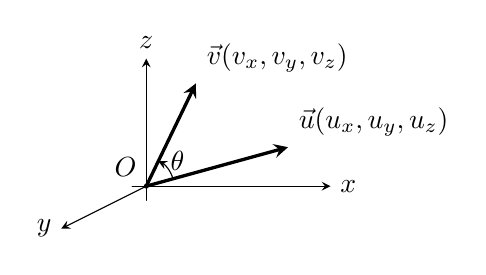
\begin{tikzpicture}[scale=0.9, line cap=round, line join=round, >=stealth]
  %--- axes (same style/orientation as your examples) ----------------------
  \draw[->] (-0.2,0) -- (2.6,0) node[right] {$x$};
  \draw[->] (0,-0.2) -- (0,1.8) node[above] {$z$};
  \draw[->] (0,0) -- (-1.2,-0.6) node[left] {$y$};

  % origin
  \coordinate (O) at (0,0);
  \fill (O) circle (1pt) node[above left] {$O$};

  %--- vectors u and v -----------------------------------------------------
  \coordinate (U) at (2.0,0.55);   % adjust to taste
  \coordinate (V) at (0.7,1.45);   % adjust to taste

  \draw[->,very thick] (O) -- (U) node[above right] {$\vec u (u_x,u_y,u_z)$};
  \draw[->,very thick] (O) -- (V) node[above right] {$\vec v (v_x,v_y,v_z)$};

  %--- angle between u and v at O -----------------------------------------
  \pic [draw,->,angle radius=10pt, angle eccentricity=1.25] {angle = U--O--V};
  \node at (0.44,0.36) {$\theta$};
\end{tikzpicture}
\end{center}
\[
\vec u \cdot \vec v \;=\; \|\vec u\|\,\|\vec v\| \cos\theta \;=\; u_x \cdot v_x + u_y \cdot v_y + u_z \cdot v_z
\]
\subsubsection{Vectorieel product van vectoren (kruisproduct)}
\[
\vec{u} \times \vec{v}
\;\stackrel{\text{def}}{=}\;
\bigl(u_y v_z - u_z v_y,\;
u_z v_x - u_x v_z,\;
u_x v_y - u_y v_x \bigr)
=\left(
\begin{vmatrix}
u_y & u_z\\
v_y & v_z
\end{vmatrix},
\begin{vmatrix}
u_z & u_x\\
v_z & v_x
\end{vmatrix},
\begin{vmatrix}
u_x & u_y\\
v_x & v_y
\end{vmatrix}
\right) \in \mathbb{R}^3
\]

\newpage

\subsection{Rechte}

\begin{table}[h!]
\centering
\begin{tabular}{|c|c|}
\hline
{\small $e \leftrightarrow
\begin{bmatrix}
x \\
y \\
z
\end{bmatrix}
=
\begin{bmatrix}
x_1 \\
y_1 \\
z_1
\end{bmatrix}
+ k \cdot
\begin{bmatrix}
a \\
b \\
c
\end{bmatrix}
$}
&
$e \leftrightarrow
\frac{x - x_1}{a}
=
\frac{y - y_1}{b}
=
\frac{z - z_1}{c}
$ \\
\hline
\end{tabular}
\end{table}

\subsection{Vlak}

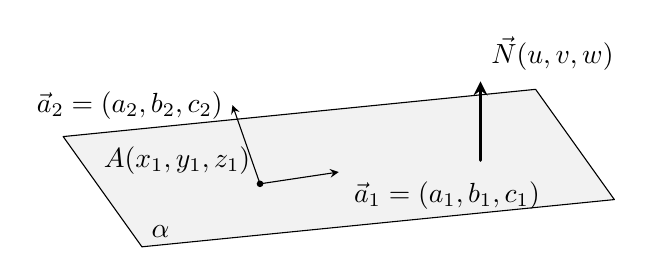
\begin{tikzpicture}[scale=1,>=stealth,line cap=round,line join=round]
  %--- Skewed plane alpha --------------------------------------------------
  \coordinate (P1) at (-3,0);
  \coordinate (P2) at ( 3,0.6);
  \coordinate (P3) at ( 2,2);
  \coordinate (P4) at (-4,1.4);

  \fill[gray!10] (P1)--(P2)--(P3)--(P4)--cycle;
  \draw (P1)--(P2)--(P3)--(P4)--cycle node[above right] {$\alpha$};

  %--- Point A and spanning vectors on the plane ---------------------------
  \coordinate (A) at (-1.5,0.8);
  \fill (A) circle (1.2pt) node[above left] {$A(x_1,y_1,z_1)$};

  % Spanning vectors a1 and a2 on the plane
  \draw[->] (A) -- ++(1.0,0.15) node[below right,xshift=2pt] {$\vec a_1=(a_1,b_1,c_1)$};
  \draw[->] (A) -- ++(-0.35,1.0) node[left] {$\vec a_2=(a_2,b_2,c_2)$};

  %--- Normal vector outside the plane -------------------------------------
  \coordinate (N) at (1.3,1.1);

  % Normal vector drawn perpendicular to the plane (upwards)
  \draw[->,very thick] (N) -- ++(0,1.0)
       node[above right] {$\vec{N}(u,v,w)$};
\end{tikzpicture}


\begin{table}[h!]
\centering
\begin{tabular}{|c|c|}
\hline
{\small $
\alpha \leftrightarrow
\begin{bmatrix}
x \\[3pt]
y \\[3pt]
z
\end{bmatrix}
=
\begin{bmatrix}
x_1 \\[3pt]
y_1 \\[3pt]
z_1
\end{bmatrix}
+ r \cdot
\begin{bmatrix}
a_1 \\[3pt]
b_1 \\[3pt]
c_1
\end{bmatrix}
+ s \cdot
\begin{bmatrix}
a_2 \\[3pt]
b_2 \\[3pt]
c_2
\end{bmatrix}
$}
&
$
\alpha \leftrightarrow
\begin{vmatrix}
x & y & z & 1 \\[3pt]
x_1 & y_1 & z_1 & 1 \\[3pt]
a_1 & b_1 & c_1 & 0 \\[3pt]
a_2 & b_2 & c_2 & 0
\end{vmatrix}
= 0
$ \\
\hline
$\alpha \leftrightarrow ux+vy+wz+t = 0 $ & $normaal \leftrightarrow \vec{N}(u, v, w)$ \\
\hline
\end{tabular}
\end{table}

\subsubsection{Snijlijn 2 vlakken}

\begin{table}[h!]
\centering
\begin{tabular}{|c|c|}
\hline
$
\begin{aligned}
\alpha &\leftrightarrow u_1x + v_1y + w_1z + t_1 = 0 \\
\beta  &\leftrightarrow u_2x + v_2y + w_2z + t_2 = 0
\end{aligned}
$
&
$
d \leftrightarrow 
\begin{cases}
u_1x + v_1y + w_1z + t_1 = 0 \\
u_2x + v_2y + w_2z + t_2 = 0
\end{cases}
$ \\
\hline
\end{tabular}
\end{table}

\subsubsection{Vlakkenwaaier van 2 vlakken}

\begin{table}[h!]
\centering
\begin{tabular}{|c|}
\hline
$
k(u_1x + v_1y + w_1z + t_1) + m(u_2x + v_2y + w_2z + t_2) = 0 
\quad (k, m \in \mathbb{R})
$
\\
\hline
\end{tabular}
\end{table}

\subsubsection{Loodlijn op een vlak / loodvlak op een rechte}

\begin{table}[h!]
\centering
\begin{tabular}{|c|c|}
\hline
$
e \leftrightarrow
\frac{x - x_1}{u}
=
\frac{y - y_1}{v}
=
\frac{z - z_1}{w}
$
& 
$
\alpha \leftrightarrow a(x - x_1) + b(y - y_1) + c(z - z_1) = 0
$
\\
\hline
\end{tabular}
\end{table}




\newpage

\subsubsection{Relatie tussen twee vlakken $\alpha,\beta$ in $\mathbb{R}^3$}
\[
\begin{aligned}
\alpha:\; u_1 x + v_1 y + w_1 z + t_1 = 0
&\qquad
\beta:\; u_2 x + v_2 y + w_2 z + t_2 = 0 \\[2mm]
\alpha_{0}:\; u_1 x + v_1 y + w_1 z = 0
&\qquad
\beta_{0}:\; u_2 x + v_2 y + w_2 z = 0
\qquad(\text{vlakken door }O)
\end{aligned}
\]

\begin{center}
\begin{minipage}[t]{0.32\linewidth}\centering
\textbf{Evenwijdig, niet samenvallend}\\[2mm]
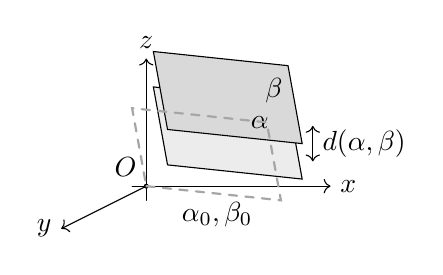
\begin{tikzpicture}[scale=0.9, line cap=round]
  % stijlen
  \tikzset{
    planeA/.style={fill=gray!15,draw},
    planeB/.style={fill=gray!30,draw},
    plane0/.style={draw=gray!70, dashed, thick}
  }
  % assen
  \draw[->] (-0.2,0) -- (2.6,0) node[right] {$x$};
  \draw[->] (0,-0.2) -- (0,1.8) node[above] {$z$};
  \draw[->] (0,0) -- (-1.2,-0.6) node[left] {$y$};
  % oorsprong
  \fill (0,0) circle (1pt) node[above left] {$O$};
  % vlakken (algemeen)
  \fill[planeA] (0.3,0.3) -- (2.2,0.1) -- (2.0,1.2) -- (0.1,1.4) -- cycle; % α
  \fill[planeB] (0.3,0.8) -- (2.2,0.6) -- (2.0,1.7) -- (0.1,1.9) -- cycle; % β
  \node at (1.6,0.9) {$\alpha$};
  \node at (1.8,1.35) {$\beta$};
  \draw[<->] (2.35,0.35) -- (2.35,0.85) node[midway,right] {$d(\alpha,\beta)$};
  % vlakken door O (parallelle kopieën)
  \draw[plane0] (0,0) -- (1.9,-0.2) -- (1.7,0.9) -- (-0.2,1.1) -- cycle; % α0
  \node at (1,-0.4) {$\alpha_{0},\beta_{0}$};
\end{tikzpicture}
\end{minipage}\hfill
%
\begin{minipage}[t]{0.32\linewidth}\centering
\textbf{Samenvallend}\\[2mm]
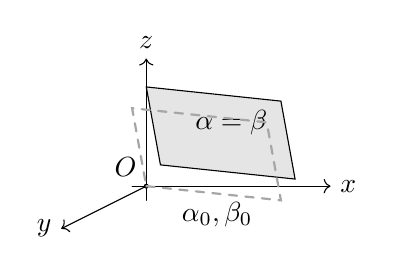
\begin{tikzpicture}[scale=0.9, line cap=round]
  \tikzset{planeC/.style={fill=gray!20,draw}, plane0/.style={draw=gray!70, dashed, thick}}
  % assen
  \draw[->] (-0.2,0) -- (2.6,0) node[right] {$x$};
  \draw[->] (0,-0.2) -- (0,1.8) node[above] {$z$};
  \draw[->] (0,0) -- (-1.2,-0.6) node[left] {$y$};
  % oorsprong
  \fill (0,0) circle (1pt) node[above left] {$O$};
  % samenvallend vlak
  \fill[planeC] (0.2,0.3) -- (2.1,0.1) -- (1.9,1.2) -- (0.0,1.4) -- cycle;
  \node at (1.2,0.9) {$\alpha=\beta$};
  % vlakken door O 
  \draw[plane0] (0,0) -- (1.9,-0.2) -- (1.7,0.9) -- (-0.2,1.1) -- cycle; % α0
  \node at (1,-0.4) {$\alpha_{0},\beta_{0}$};
\end{tikzpicture}
\end{minipage}\hfill
%
\begin{minipage}[t]{0.32\linewidth}\centering
\textbf{Snijdend (lijn)}\\[2mm]
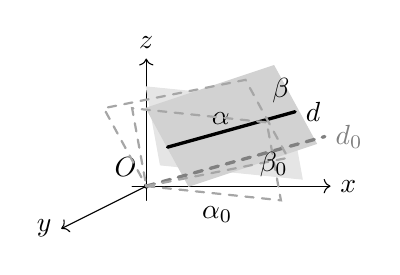
\begin{tikzpicture}[scale=0.9, line cap=round]
  \tikzset{plane0/.style={draw=gray!70, dashed, thick}}
  % assen
  \draw[->] (-0.2,0) -- (2.6,0) node[right] {$x$};
  \draw[->] (0,-0.2) -- (0,1.8) node[above] {$z$};
  \draw[->] (0,0) -- (-1.2,-0.6) node[left] {$y$};
  % oorsprong
  \fill (0,0) circle (1pt) node[above left] {$O$};
  % vlakken (algemeen)
  \fill[gray!20,draw] (0.2,0.3) -- (2.2,0.1) -- (2.0,1.2) -- (0.0,1.4) -- cycle; % α
  \fill[gray!35,draw] (0.6,0.0) -- (2.4,0.6) -- (1.8,1.7) -- (0.0,1.1) -- cycle; % β
  \node at (1.05,0.95) {$\alpha$};
  \node at (1.9,1.35) {$\beta$};
% snijlijn d
  \draw[very thick] (0.3,0.55) -- (2.1,1.05) node[right] {$d$};

% evenwijdige door O: d_0  (zelfde richting als d)
  \draw[gray,very thick, dashed] (0,0) -- (2.52,0.70) node[right] {$d_{0}$};
  
  % door O: α0 en β0 als gestreepte vlakken
  \draw[plane0] (0,0) -- (1.9,-0.2) -- (1.7,0.9) -- (-0.2,1.1) -- cycle; % α0
  \draw[plane0] (0,0) -- (2.0,0.4) -- (1.4,1.5) -- (-0.6,1.1) -- cycle;   % β0
  \node at (1,-0.4) {$\alpha_{0}$};
  \node at (1.8,0.3) {$\beta_{0}$};
\end{tikzpicture}
\end{minipage}
\end{center}



\begin{center}
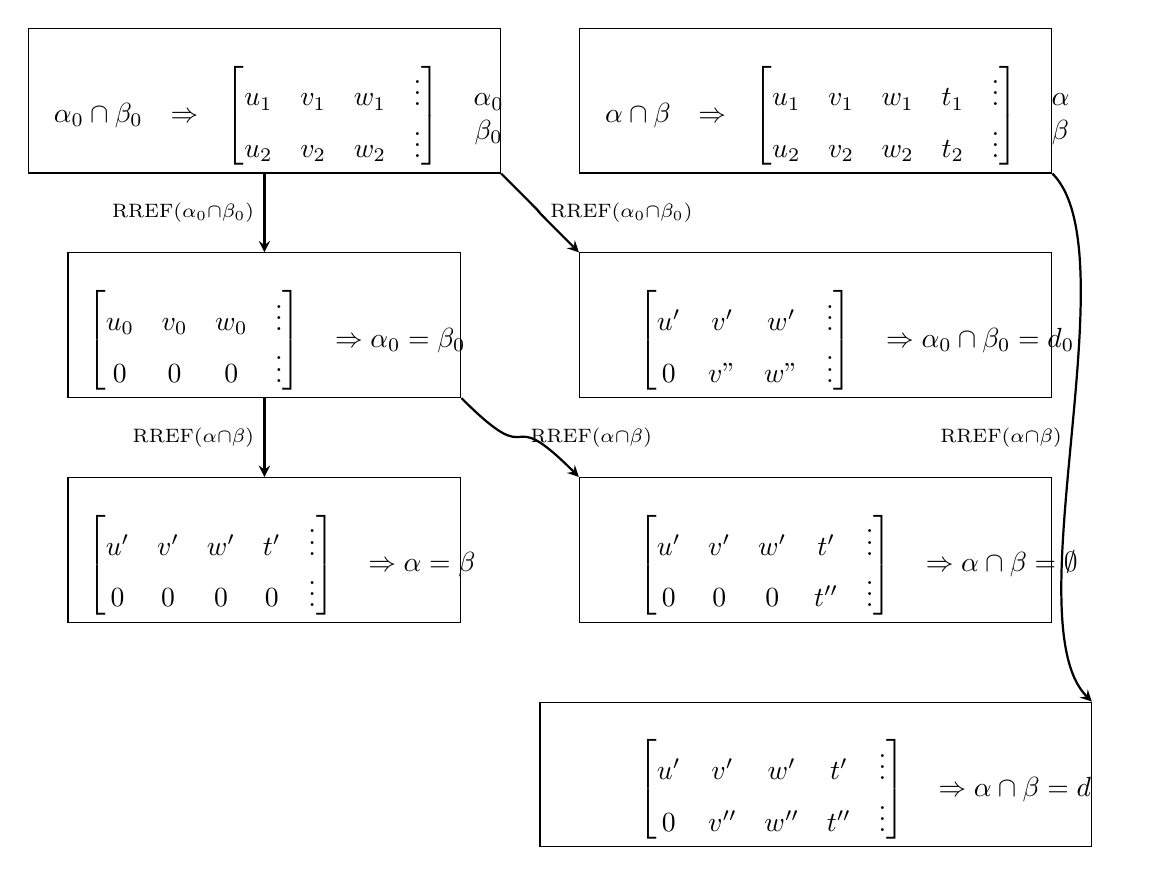
\begin{tikzpicture}[>=stealth]
% ----------------- First row -----------------
\node (box1) [draw, inner sep=2pt, minimum width=6cm, anchor=north west] at (0,0) {
\begin{minipage}{0.47\linewidth}
\[
\begin{array}{c c c}
\alpha_0 \cap \beta_0 & \Rightarrow &
\begin{bmatrix}
u_{1} & v_{1} & w_{1} & \vdots \\
u_{2} & v_{2} & w_{2} & \vdots
\end{bmatrix}
\;\;
\begin{array}{c}
\alpha_{0} \\
\beta_{0}
\end{array}
\end{array}
\]
\end{minipage}
};

\node (box2) [draw, inner sep=2pt, minimum width=6cm, anchor=north west] at (7,0) {
\begin{minipage}{0.47\linewidth}
\[
\begin{array}{c c c}
\alpha \cap \beta & \Rightarrow &
\begin{bmatrix}
  u_{1} & v_{1} & w_{1} & t_{1} & \vdots \\
  u_{2} & v_{2} & w_{2} & t_{2} & \vdots
\end{bmatrix}
\;\;
\begin{array}{c}
  \alpha \\
  \beta
\end{array}
\end{array}
\]
\end{minipage}
};


% ----------------- Second row (copy) -----------------
\node (box3) [draw, inner sep=2pt, minimum width=4cm, below=1cm of box1] {
  \begin{minipage}{0.4\linewidth}
  \[
  \begin{array}{c}
  \begin{bmatrix}
  u_{0} & v_{0} & w_{0} & \vdots \\
  0 & 0 & 0 & \vdots
  \end{bmatrix}
  \;\;
  \begin{array}{c}
  \Rightarrow \alpha_{0}=\beta_{0}
  \end{array}
  \end{array}
  \]
  \end{minipage}
};

\node (box4) [draw, inner sep=2pt, minimum width=6cm, below=1cm of box2] {
  \begin{minipage}{0.4\linewidth}
  \[
  \begin{array}{c}
  \begin{bmatrix}
  u' & v' & w' & \vdots \\
   0 & v" & w" & \vdots
  \end{bmatrix}
  \;\;
  \begin{array}{c}
  \Rightarrow \alpha_0 \cap \beta_0 = d_{0}
  \end{array}
  \end{array}
  \]
  \end{minipage}
};

% ----------------- row 3 -----------------
\node (box5) [draw, inner sep=2pt, minimum width=4cm, below=1cm of box3] {
  \begin{minipage}{0.4\linewidth}
  \[
  \begin{array}{c}
  \begin{bmatrix}
  u' & v' & w' & t' & \vdots \\
  0  & 0  & 0  & 0  & \vdots
  \end{bmatrix}
  \;\;
  \begin{array}{c}
  \Rightarrow \alpha=\beta
  \end{array}
  \end{array}
  \]
  \end{minipage}
};

\node (box6) [draw, inner sep=2pt, minimum width=6cm, below=1cm of box4] {
 \begin{minipage}{0.4\linewidth}
  \[
  \begin{array}{c}
  \begin{bmatrix}
  u' & v' & w' & t'  & \vdots \\
  0  & 0  & 0  & t'' & \vdots
  \end{bmatrix}
  \;\;
  \begin{array}{c}
  \Rightarrow \alpha \cap \beta = \emptyset
  \end{array}
  \end{array}
  \]
  \end{minipage}
};

\node (box7) [draw, inner sep=2pt, minimum width=7cm, below=1cm of box6] {
 \begin{minipage}{0.4\linewidth}
  \[
  \begin{array}{c}
  \begin{bmatrix}
  u' & v' & w' & t'  & \vdots \\
  0  & v''  & w''  & t'' & \vdots
  \end{bmatrix}
  \;\;
  \begin{array}{c}
  \Rightarrow \alpha \cap \beta = d
  \end{array}
  \end{array}
  \]
  \end{minipage}
};


% ----------------- Arrows -----------------
\draw[->, thick] (box1.south) .. controls +(0,-1) and +(0,1) .. (box3.north)node[midway, left] {$\scriptstyle \mathrm{RREF} (\alpha_0 \cap \beta_0)$};
\draw[->, thick] (box1.south east) .. controls +(1,-1) and +(-1,1) .. (box4.north west)node[midway, right] {$\scriptstyle \mathrm{RREF} (\alpha_0 \cap \beta_0)$};

\draw[->, thick] (box3.south) .. controls +(0,-1) and +(0,1) .. (box5.north)node[midway, left] {$\scriptstyle \mathrm{RREF} (\alpha \cap \beta)$};
\draw[->, thick] (box3.south east) .. controls +(1,-1) and +(-1,1) .. (box6.north west)node[midway, right] {$\scriptstyle \mathrm{RREF} (\alpha \cap \beta)$};

\draw[->, thick] (box2.south east) .. controls +(1,-1) and +(-1,1) .. (box7.north east)node[midway, left] {$\scriptstyle \mathrm{RREF} (\alpha \cap \beta)$};

\end{tikzpicture}
\end{center}

\newpage

\subsection{Bol}
Bol met middelpunt $M(x_M,y_M,z_M)\;en\;straal=r$
\[
\boxed{(x-x_M)^2 + (y-y_M)^2 + (z-z_M)^2 = r^2}
\]

\[
\begin{aligned}
x^2 + y^2 + z^2 + 2ax + 2by + 2cz + d &= 0 \\
\land \quad a^2 + b^2 + c^2 - d &\ge 0
\end{aligned}
\]
\[
\Downarrow
\]
\[
\text{M}(-a, -b, -c) \quad\text{en}\quad r = \sqrt{a^2 + b^2 + c^2 - d}
\]

\newpage

\subsection{Basis reële functies}

\begin{tabular}{|m{0.3\textwidth}|m{0.6\textwidth}|}
\hline
\textbf{Functie} & \textbf{Definitie} \\
\hline
Identiteitsfunctie & $ f(x) = x $ \\
\hline
Constante functie & $ f(x) = c, \; c \in \mathbb{R} $ \\
\hline
Lineaire functie & $ f(x) = mx + b, \; m, b \in \mathbb{R} $ \\
\hline
Kwadratische functie & $ f(x) = ax^2 + bx + c, \; a, b, c \in \mathbb{R}, \; a \neq 0 $ \\
\hline
Cubische functie & $ f(x) = ax^3 + bx^2 + cx + d, \; a, b, c, d \in \mathbb{R}, \; a \neq 0 $ \\
\hline
Polynoomfunctie & $ f(x) = a_n x^n + a_{n-1} x^{n-1} + \dots + a_1 x + a_0, \; a_i \in \mathbb{R} \newline a_n \neq 0 $ \\
\hline
Rationale functie & $ f(x) = \frac{P(x)}{Q(x)}, \; P(x), Q(x) \text{ zijn polynomen}, \; Q(x) \neq 0 $ \\
\hline
Exponenti\"ele functie & $ f(x) = a^x, \; a > 0, \; a \neq 1 $\\
\hline
Logaritmische functie & $ f(x) = \log_a(x), \; a > 0, \; a \neq 1, \; x > 0 $ \\
\hline
Absolute-waarde functie & $
    f(x) = |x| =
    \begin{cases}
    x, & x \geq 0 \\
    -x, & x < 0
    \end{cases}
$ \\
\hline
Goniometrische functies & $
	f(x) = \sin(x) \newline
	f(x) = \cos(x) \newline
	f(x) = \tan(x) \; x \neq \frac{\pi}{2} + k\pi, \; k \in \mathbb{Z}
$ \\
\hline
Inverse goniometrische functies & $
	f(x) = \arcsin(x), \; x \in [-1, 1] \newline
	f(x) = \arccos(x), \; x \in [-1, 1] \newline
	f(x) = \arctan(x), \; x \in \mathbb{R}$ \\
\hline
Hyperbolische functies & $
    f(x) = \sinh(x) = \frac{e^x - e^{-x}}{2} \newline
    f(x) = \cosh(x) = \frac{e^x + e^{-x}}{2} \newline
    f(x) = \tanh(x) = \frac{\sinh(x)}{\cosh(x)}, \; x \in \mathbb{R}
\) \\
\hline
Stukjesfunctie & $
    f(x) =
    \begin{cases}
    x^2, & x < 0 \\
    x + 1, & x \geq 0
    \end{cases}
$ \\
\hline
\end{tabular}

\newpage

\section{Analyse}
\subsection{Limieten van rijen)}
\fontsize{14pt}{15pt}\selectfont
$\begin{array}{|l|}
\hline
\mathop {\lim }\limits_{n \to  \pm \infty } \left( {{a_m}{n^m} + {a_{m - 1}}{n^{m - 1}} + ... + {a_1}n + {a_0}} \right) = \mathop {\lim }\limits_{n \to  \pm \infty } {a_m}{n^m}\\
\hline
\mathop {\lim }\limits_{n \to  \pm \infty } \frac{{\left( {{a_m}{n^m} + {a_{m - 1}}{n^{m - 1}} + ... + {a_1}n + {a_0}} \right)}}{{\left( {{b_q}{n^p} + {b_{q - 1}}{n^{p - 1}} + ... + {b_1}n + {b_0}} \right)}} = \mathop {\lim }\limits_{n \to  \pm \infty } \frac{{{a_m}{n^m}}}{{{b_q}{n^p}}} \\
\hline
\end{array}$
\normalsize
\subsection{Limieten van functies}
\fontsize{14pt}{15pt}\selectfont
$\begin{array}{|l|}
\hline
\mathop {\lim }\limits_{x \to a} \left[ {f\left( x \right) \pm g\left( x \right)} \right] = \mathop {\lim }\limits_{x \to a} f\left( x \right) \pm \mathop {\lim }\limits_{x \to a} g\left( x \right)\\
\hline
\mathop {\lim }\limits_{x \to a} \left[ {f\left( x \right).g\left( x \right)} \right] = \mathop {\lim }\limits_{x \to a} f\left( x \right).\mathop {\lim }\limits_{x \to a} g\left( x \right)\\
\hline
\mathop {\lim }\limits_{x \to a} {\left[ {f\left( x \right)} \right]^n} = {\left[ {\mathop {\lim }\limits_{x \to a} f\left( x \right)} \right]^n}\quad \quad \left( {n \in {_0}} \right)\\
\hline
\mathop {\lim }\limits_{x \to a} \sqrt[n]{{f\left( x \right)}} = \sqrt[n]{{\mathop {\lim }\limits_{x \to a} f\left( x \right)}}\\
\hline
\mathop {\lim }\limits_{x \to a} \frac{{f\left( x \right)}}{{g\left( x \right)}} = \frac{{\mathop {\lim }\limits_{x \to a} f\left( x \right)}}{{\mathop {\lim }\limits_{x \to a} g\left( x \right)}}\\
\mathop {\lim }\limits_{x \to  \pm \infty } \left( {{a_n}{x^n} + {a_{n - 1}}{x^{n - 1}} + ... + {a_1}x + {a_0}} \right) = \mathop {\lim }\limits_{x \to  \pm \infty } {a_n}{x^n}\\
\hline
\mathop {\lim }\limits_{x \to  \pm \infty } \frac{{{a_n}{x^n} + {a_{n - 1}}{x^{n - 1}} + ... + {a_1}x + {a_0}}}{{{b_m}{x^m} + {b_{m - 1}}{x^{m - 1}} + ... + {b_1}x + {b_0}}} = \mathop {\lim }\limits_{x \to  \pm \infty } \frac{{{a_n}{x^n}}}{{{b_m}{x^m}}} \\
\hline
\end{array}$

\subsection{Limieten van goniometrische functies}

$\begin{array}{|l|l|}
\hline
\begin{array}{l}
\mathop {\lim }\limits_{x \to a} \sin (x) = \sin (a)\\
\mathop {\lim }\limits_{x \to a} \cos (x) = \cos (a)
\end{array}
&
\begin{array}{l}
\mathop {\lim }\limits_{x \to 0} \frac{{\sin x}}{x} = 1\\
\mathop {\lim }\limits_{x \to 0} \frac{{\tan x}}{x} = 1
\end{array} \\
\hline
\end{array}$
\normalsize

\newpage

\subsection{Methodes bij het berekenen van limieten van functies}
\par\vspace{0.3cm}
% 
% VEELTERM F
%
\underline{Veeltermfunctie :} $\mathop {\lim }\limits_{x \to a} f\left( x \right) = $ Eindige a	limiet = functiewaarde \newline
Oneindige a	limiet = limiet van de hoogstegraadsterm \newline
\par\vspace{0.3cm}
% 
% RAT. F
%
\underline{Gebroken rationale functie :} \newline
Eindige a \newline
\begin{tabularx}{\textwidth}{|>{\centering\arraybackslash}m{3.5cm}|X|}
\hline
\( a \in \mathrm{dom} \, f(x) \) & limiet = functiewaarde \\
\hline
\textbf{geval} \( \frac{r}{0} \land r \in \mathbb{R} \) & linker- en rechterlimiet zijn \( \infty \); teken afleiden uit het teken van \( r \) en de noemer \\
\hline
\textbf{geval} \( \frac{0}{0} \) & deel teller en noemer door \( (x - a) \), bereken de limiet van de bekomen functie \\
\hline
\end{tabularx}
Oneindige \( a \)\newline
\begin{tabularx}{\textwidth}{|X|}
\hline
limiet = limiet van quotiënt hoogste graadstermen \\
\hline
\end{tabularx}
\par\vspace{0.3cm}
% 
% IRRAT. F
%
\underline{Irrationale functie :} \newline
Eindige a \newline
\begin{tabularx}{\textwidth}{|>{\centering\arraybackslash}m{4.5cm}|X|}
\hline
\( a \in \mathrm{dom} \, f(x) \) & limiet = functiewaarde \\
\hline
\begin{tabular}[c]{@{}c@{}}%
\( a \in \mathrm{adh} \, \mathrm{dom} \, f(x) \) \\
\( \displaystyle \frac{r}{0} \land r \in \mathbb{R} \)
\end{tabular} 
& linker- en rechterlimiet zijn \( \infty \); teken afleiden uit het teken van \( r \) en de noemer \\
\hline
\begin{tabular}[c]{@{}c@{}}%
\( a \in \mathrm{adh} \, \mathrm{dom} \, f(x) \) \\
\( \displaystyle \frac{0}{0} \land r \in \mathbb{R} \)
\end{tabular} 
& vermenigvuldig teller en noemer met de toegevoegde wortelvorm, deel teller en noemer door $\left( {x - a} \right)$ , bereken de limiet van de bekomen functie \\
\hline
\( a \notin \mathrm{adh} \, \mathrm{dom} \, f(x) \)
& geen limiet \\
\hline
\end{tabularx}
Oneindige \( a \) \newline
\begin{tabularx}{\textwidth}{|>{\centering\arraybackslash}m{4.5cm}|X|}
\hline
\( \pm \infty \in \mathrm{adh} \, \mathrm{dom} \, f(x) \) en \( f(\pm \infty) \) is te berekenen 
& limiet = resultaat berekening \\
\hline
\( \pm \infty \in \mathrm{adh} \, \mathrm{dom} \, f(x) \) \newline geval \( \dfrac{\infty}{\infty} \) 
& zet in de teller en de noemer de hoogste macht van \( x \) voorop, vereenvoudig en bereken de limiet van de bekomen functie \\
\hline
\( \pm \infty \in \mathrm{adh} \, \mathrm{dom} \, f(x) \) \newline geval \( \infty - \infty \)
& herleid tot het vorige geval door teller en noemer te vermenigvuldigen met de toegevoegde wortelvorm \\
\hline
\( a \notin \mathrm{adh} \, \mathrm{dom} \, f(x) \) 
& geen limiet \\
\hline
\end{tabularx}
\par\vspace{0.3cm}
% 
% Hopital
%
\underline{Regel l’Hôptal:} \newline
\begin{tabularx}{\textwidth}{|X|}
\hline
$\begin{array}{l}
\mathop {\lim }\limits_{x \to a} f\left( x \right) = \mathop {\lim }\limits_{x \to a} g\left( x \right) = \;0\;\; \vee \;\; \pm \infty \\
\mathop {\lim }\limits_{x \to a} \frac{{f\left( x \right)}}{{g\left( x \right)}} = \mathop {\lim }\limits_{x \to a} \frac{{f'\left( x \right)}}{{g'\left( x \right)}}
\end{array}$ \\
\hline
\end{tabularx}

\newpage

\par\vspace{0.3cm}
\underline{Bewerkingen met oneindig en onbepaalde vormen:} \newline

\begin{tabular}{|>{\centering\arraybackslash}m{6.5cm}|>{\centering\arraybackslash}m{5cm}|}
\hline
\textbf{Bewerkingen} & \textbf{Geen betekenis} \\ \hline

\( x + (-\infty) = -\infty + x = (-\infty) + x \) &
\( (+\infty) + (-\infty) \) \\ \hline

\( x + (+\infty) = +\infty + x = (+\infty) + x \) &
\( (-\infty) + (+\infty) \) \\ \hline

\( x \cdot (+\infty) = (+\infty) \cdot x = +\infty \) als \( x > 0 \) &
\( 0 \cdot (+\infty), (+\infty) \cdot 0 \) \\ \hline

\( x \cdot (+\infty) = (+\infty) \cdot x = -\infty \) als \( x < 0 \) &
\( 0 \cdot (-\infty), (-\infty) \cdot 0 \) \\ \hline

\( x \cdot (-\infty) = (-\infty) \cdot x = -\infty \) als \( x > 0 \) &
\( \frac{1}{0} \) \\ \hline

\( x \cdot (-\infty) = (-\infty) \cdot x = +\infty \) als \( x < 0 \) &
\( 1^{+\infty} \) \\ \hline

\( (+\infty) + (+\infty) = +\infty \) &
\( 0^0 \) \\ \hline

\( (-\infty) + (-\infty) = -\infty \) &
\( (+\infty)^0 \) \\ \hline

\( (+\infty) \cdot (+\infty) = (-\infty) \cdot (-\infty) = +\infty \) &
\\ \hline

\( (+\infty) \cdot (-\infty) = (-\infty) \cdot (+\infty) = -\infty \) &
\\ \hline

\( (+\infty)^n = +\infty \) als \( n \) even is &
\\ \hline

\( (-\infty)^n = -\infty \) als \( n \) oneven is &
\\ \hline

\( \frac{1}{+\infty} = \frac{1}{-\infty} = 0 \) &
\\ \hline

\( \sqrt[n]{+\infty} = +\infty \) &
\\ \hline

\( \sqrt[n]{-\infty} = -\infty \) als \( n \) oneven is &
\\ \hline

\end{tabular}

\subsection{Afgeleiden}
\fontsize{13pt}{14pt}\selectfont
\[f'(a)
= \lim_{\scriptscriptstyle \Delta x \to 0} \frac{\Delta y}{\Delta x}
= \lim_{\scriptscriptstyle \Delta x \to 0} \frac{f(a + \Delta x) - f(a)}{\Delta x}
= \lim_{\scriptscriptstyle x \to a} \frac{f(x) - f(a)}{x - a}
= \left( \frac{df}{dx} \right)_{x=a}
\\
\]
\normalsize
\[g(x) = u, \qquad D_x\!\bigl[f(g(x))\bigr]
= D_x\!\bigl[f(u)\bigr]
= \frac{d[f(u)]}{dx}
= \frac{d[f(u)]}{du} \cdot \frac{du}{dx}
= D_u\!\bigl[f(u)\bigr] \cdot D_x\!\bigl[u\bigr]\]

\subsubsection{Differentiaal}
\[
df(x)=Df(x)\cdot dx
\]

\subsubsection{Partiële afgeleiden en totale differentiaal}
\begin{tabular}{@{}p{0.60\linewidth}@{\hspace{1em}}p{0.40\linewidth}@{}}
% -------------------- LEFT COLUMN --------------------
\noindent
\begin{minipage}[c]{\linewidth}
\[
z = f(x,y)
\Rightarrow
\begin{cases}
  \dfrac{\partial f}{\partial x}
    = \displaystyle\lim_{\scriptscriptstyle \Delta x \to 0}
      \dfrac{f(x+\Delta x, y)-f(x,y)}{\Delta x} \\[1em]
  \dfrac{\partial f}{\partial y}
    = \displaystyle\lim_{\scriptscriptstyle \Delta y \to 0}
      \dfrac{f(x, y+\Delta y)-f(x,y)}{\Delta y}
\end{cases}
\]
\[
dz = \dfrac{\partial f}{\partial x}\,dx + \dfrac{\partial f}{\partial y}\,dy
\]
\end{minipage}\hfill
&
% -------------------- RIGHT COLUMN --------------------
\begin{minipage}[r]{\linewidth}
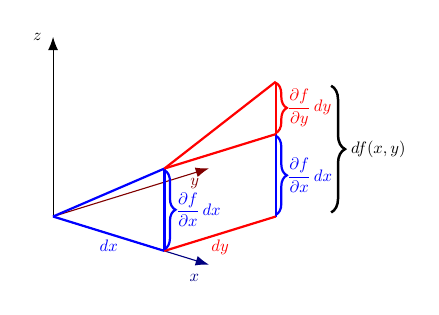
\begin{tikzpicture}[
  3d view={45}{18},
  >=Latex, thick,
  dx/.style={draw, line width=0.9pt, color=blue},
  dy/.style={draw, line width=0.9pt, color=red},
  df/.style={draw, line width=0.9pt, color=green!50!black},
  note/.style={scale=0.6}
]
  \def\Bx{2} \def\By{2}
  \def\ax{0.55}
  \def\ay{0.35}

  % Base rectangle (z=0)
  \coordinate (A) at (tpp cs:x=0,y=0,z=0);
  \coordinate (B) at (tpp cs:x=\Bx,y=0,z=0);
  \coordinate (C) at (tpp cs:x=\Bx,y=\By,z=0);
  \coordinate (D) at (tpp cs:x=0,y=\By,z=0);

  % only the x-change
  \coordinate (Ap) at (tpp cs:x=0,y=0,z=\ax*\Bx);
  \coordinate (Bp) at (tpp cs:x=\Bx,y=0,z=\ax*\Bx);
  \coordinate (Cp) at (tpp cs:x=\Bx,y=\By,z=\ax*\Bx);
  \coordinate (Dp) at (tpp cs:x=0,y=\By,z=\ax*\Bx);

  % the y-change
  \coordinate (A1) at (tpp cs:x=0,y=0,z=\ax*\Bx);
  \coordinate (B1) at (tpp cs:x=\Bx,y=0,z=\ax*\Bx);
  \coordinate (C1) at (tpp cs:x=\Bx,y=\By,z={(\ax*\Bx)+(\ay*\By)});
  \coordinate (D1) at (tpp cs:x=0,y=\By,z={(\ax*\Bx)+(\ay*\By)});

  % Axes
  \draw[->, thin, blue!50!black]  (tpp cs:x=0,y=0,z=0) -- (tpp cs:x=2.8,y=0,z=0)
      node[below left=2pt, note] {$x$};
  \draw[->, thin, red!50!black]   (tpp cs:x=0,y=0,z=0) -- (tpp cs:x=0,y=2.8,z=0)
      node[below left=2pt, note] {$y$};
  \draw[->, thin, black!50!black] (tpp cs:x=0,y=0,z=0) -- (tpp cs:x=0,y=0,z=2.4)
      node[left=2pt, note] {$z$};

  % Geometry
  \draw[blue] (A)--(B) node[midway, below, note, blue] {$dx$};
  \draw[blue] (A)--(Bp);
  \draw[blue] (B)--(Bp);
  \draw[blue] (C)--(Cp);

  % right wall
  \draw[red] (B)--(C) node[midway, below, note, red] {$dy$};
  \draw[red] (Bp)--(Cp);
  \draw[red] (Bp)--(C1);
  \draw[red] (Cp)--(C1);

  % braces and labels
  \draw[decorate, decoration={brace, mirror, amplitude=4pt}, blue]
    ($(B)!0.02!(Bp)$) --
    node[right=2pt, note, text=blue]{$\displaystyle \frac{\partial f}{\partial x}\,dx$}
    ($(B)!0.98!(Bp)$);
    
   \draw[decorate, decoration={brace, mirror, amplitude=4pt}, blue]
    ($(C)!0.02!(Cp)$) --
    node[right=2pt, note, text=blue]{$\displaystyle \frac{\partial f}{\partial x}\,dx$}
    ($(C)!0.98!(Cp)$);

  \draw[decorate, decoration={brace, mirror, amplitude=4pt}, red]
    ($(Cp)!0.02!(C1)$) --
    node[right=2pt, note, text=red]{$\displaystyle \frac{\partial f}{\partial y}\,dy$}
    ($(Cp)!0.98!(C1)$);

  \draw[df, decorate, decoration={brace,mirror, raise=20pt, amplitude=5pt}, black ]
    ($(C)!0.03!(C1)$) --
    node[midway,right=25pt, note]{$\displaystyle df(x,y)$}
    ($(C)!0.97!(C1)$);
\end{tikzpicture}
\end{minipage}
\\
\end{tabular}

\newpage


\subsubsection{Afgeleiden - differentialen}
\fontsize{14pt}{15pt}\selectfont
\[
\begin{array}{|l|l|}
\hline
Dc = 0, \; D(c f) = c Df & df = 0 \\
\hline
D(f \pm g) = Df \pm Dg & d(f \pm g) = df \pm dg \\
\hline
D(fg) = f Dg + g Df & d(fg) = f\,dg + g\,df \\
\hline
D\!\left(\frac{f}{g}\right) = \frac{gDf - fDg}{g^2} & d\!\left(\frac{f}{g}\right) = \frac{g\,df - f\,dg}{g^2} \\
\hline
D(x^n) = n x^{n-1} & d(x^n) = n x^{n-1} dx \\
\hline
D(\sin x) = \cos x & d(\sin x) = \cos x\,dx \\
\hline
D(\cos x) = -\sin x & d(\cos x) = -\sin x\,dx \\
\hline
D(\tan x) = \sec^2 x = \frac{1}{\cos^2 x} & d(\tan x) = \sec^2 x\,dx = \frac{dx}{\cos^2 x} \\
\hline
D(\cot x) = -\csc^2 x = -\frac{1}{\sin^2 x} & d(\cot x) = -\csc^2 x\,dx = -\frac{dx}{\sin^2 x} \\
\hline
D(\arcsin x) = \frac{1}{\sqrt{1-x^2}} & d(\arcsin x) = \frac{dx}{\sqrt{1-x^2}} \\
\hline
D(\arccos x) = \frac{-1}{\sqrt{1-x^2}} & d(\arccos x) = \frac{-dx}{\sqrt{1-x^2}} \\
\hline
D(\arctan x) = \frac{1}{1+x^2} & d(\arctan x) = \frac{dx}{1+x^2} \\
\hline
D(\sinh x) = \cosh x & d(\sinh x) = \cosh x\,dx \\
\hline
D(\cosh x) = \sinh x & d(\cosh x) = \sinh x\,dx \\
\hline
D(\tanh x) = \frac{1}{\cosh^2 x} & d(\tanh x) = \frac{dx}{\cosh^2 x} \\
\hline
D(e^x)=e^x,\:D(a^x)=a^x \ln a & d(e^x)=e^x\,dx,\:d(a^x)=a^x \ln a\,dx \\
\hline
D(\ln x) = \frac{1}{x}, \quad D(\ln|x|) = \frac{1}{x} & d(\ln|x|) = \frac{dx}{x} \\
\hline
D({}^a\!\log x) = \frac{1}{x \ln a} & d({}^a\!\log x) = \frac{dx}{x \ln a} \\
\hline
D\!\left(\ln|x + \sqrt{x^2 + k}|\right) = \frac{1}{\sqrt{x^2 + k}} &
d\!\left(\ln|x + \sqrt{x^2 + k}|\right) = \frac{dx}{\sqrt{x^2 + k}} \\
\hline
D(u^v) = v u^{v-1} Du + u^v \ln u\, Dv &
d(u^v) = v u^{v-1} du + u^v \ln u\, dv \\
\hline
\end{array}
\]
\normalsize

\newpage

\subsection{Afgeleiden - fundamentele integralen}
\vspace{2mm}
Bg = arc
\vspace{2mm}
\newline
\fontsize{14pt}{15pt}\selectfont
$
\begin{array}{|l|l|}
\hline
\textbf{Afgeleiden} & \textbf{Integraal} \\
\hline
D[c] = 0 & \int dx = x + C \\
\hline
D[x^n] = n x^{n-1} & \int x^n dx = \frac{x^{n+1}}{n+1} + C \quad (n \neq -1) \\
\hline
D[\sin x] = \cos x & \int \cos x \, dx = \sin x + C \\
\hline
D[\cos x] = -\sin x & \int \sin x \, dx = -\cos x + C \\
\hline
D[\tan x] = \sec^2 x = \frac{1}{{{{\cos }^2}x}} & \int \frac{1}{{{{\cos }^2}x}} \, dx = \tan x + C \\
\hline
D[\cot x] = -\csc^2 x = \frac{-1}{{{{\sin }^2}x}} & \int \frac{1}{{{{\sin }^2}x}} \, dx = -\cot x + C \\
\hline
D[\arcsin x] = \frac{1}{\sqrt{1-x^2}} & \int \frac{dx}{\sqrt{1-x^2}} = \arcsin x + C \\
\hline
D[\arccos x] = \frac{-1}{\sqrt{1-x^2}} & \int \frac{dx}{\sqrt{1-x^2}} = -\arccos x + C \\
\hline
D[\arctan x] = \frac{1}{1+x^2} & \int \frac{dx}{1+x^2} = \arctan x + C \\
\hline
D[e^x] = e^x & \int e^x dx = e^x + C \\
\hline
D[a^x] = a^x \ln a & \int a^x dx = \frac{a^x}{\ln a} + C \\
\hline
D[\ln x] = \frac{1}{x} & \int \frac{dx}{x} = \ln |x| + C \\
\hline
D\left[\ln \left| x + \sqrt{x^2 + k} \right| \right] = \frac{1}{\sqrt{x^2 + k}} & \int \frac{dx}{\sqrt{x^2 + k}} = \ln \left| x + \sqrt{x^2 + k} \right| + C \\
\hline
D{}^a\log x = \frac{1}{{x\ln a}} & * \\
\hline
\end{array}
$
\normalsize

\vspace{2mm}

\subsection{Partiële integratie}
\vspace{2mm}
\fontsize{14pt}{15pt}\selectfont
$\int {f(x)\;d(g(x)} ) = f(x).g(x) - \int {g(x)\;d(f(x)} )$
\vspace{2mm}
\newline
$\int {u\;dv}  = u.v - \int {v\;du} $
\normalsize

\newpage

\subsection{Integralen}
\subsubsection{Formules voor goniometrische integralen}

\begin{tabular}{|p{0.98\linewidth}|}
\hline
\vspace{-18pt}% optional adjustment
\[
\begin{aligned}
\int \sin^{m}x \,\cos^{n}x \, dx \qquad m,n\in\mathbb{Z}
\end{aligned}
\]
\vspace{-14pt}% optional adjustment
\\
\hline
\vspace{-7pt}% optional adjustment

% --- Row 2: split into 2 columns ---
\begin{tabular}{|p{0.2\linewidth}|p{0.73\linewidth}|}
\hline
$\begin{aligned}
&m \; \vee \; n \; oneven\\
&substitutie\\
&t=\sin x\;\vee\;\cos x\\
&\sin^{2}x+\cos^{2}x=1
\end{aligned}$
&
% --- 2nd cell: nested tabular with title "m ^ n even" and 2 columns ---
\begin{tabular}{|p{0.3\linewidth}|p{0.63\linewidth}|}
\hline
\multicolumn{2}{|c|}{$\;m\;\wedge\;n\;\text{even}\;$}\\
\hline
$\begin{aligned}
&m\;\wedge\;n\;\text{positief}\\
&\sin^{2}\alpha=\dfrac{1-\cos 2\alpha}{2}\\
&\cos^{2}\alpha=\dfrac{1+\cos 2\alpha}{2}
\end{aligned}$
&
$\begin{aligned}
&m\;\vee\;n\;\text{negatief} \\
&\frac{dx}{\cos x}=d(\tan x)\;\;\vee\;\;\frac{dx}{\sin x}=-\,d(\cot x)\\
&eventueel\\
&\tan^{2}\alpha+1=\sec^{2}\alpha,\; 1+\cot^{2}\alpha=\csc^{2}\alpha
\end{aligned}$
\\
\hline

\end{tabular}
\\
\hline

\end{tabular}
\\
\hline
\vspace{2pt}% optional adjustment

% --- Row 3: integrals with sec, tan, cot ---
$\begin{aligned}
&\int \sec x\,dx=\int \frac{\cos x\,dx}{\cos x}
\qquad \wedge\; \sin x=t
\qquad \int \sec^{2}x\,dx=\int \frac{1}{\cos^{2}x}\,dx\\
&\int \sec^{3}x\,dx =\int \sec^{2}x\cdot \sec x\,dx =\int \sec x\,d(\tan x)\;\xrightarrow{\;P.I\;}\; \cdots \xrightarrow{\;\text{terugkeer v/d integrand}\;}\; \cdots\\
&\int \tan x\,dx=-\ln|\cos x|+c \quad ,\quad \int \cot x\,dx=\ln|\sin x|+c\\
&\int \tan^{n}x\,dx\;,\;\; \int \cot^{n}x\,dx \quad n\in\mathbb{N}_0\setminus\{1\}\\
&\tan^{2}\alpha+1=\sec^{2}\alpha\;,\qquad 1+\cot^{2}\alpha=\csc^{2}\alpha
\end{aligned}$
\\
\hline
% --- Row 4: product-to-sum formulas ---
\[
\begin{aligned}
\sin(mx)\cos(nx)&=\tfrac12\!\left[\sin\!\big(mx-nx\big)+\sin\!\big(mx+nx\big)\right]\\[6pt]
\cos(mx)\cos(nx)&=\tfrac12\!\left[\cos\!\big(mx-nx\big)+\cos\!\big(mx+nx\big)\right]\\[6pt]
\sin(mx)\sin(nx)&=\tfrac12\!\left[\cos\!\big(mx-nx\big)-\cos\!\big(mx+nx\big)\right]
\end{aligned}
\]
\vspace{-7pt}% optional adjustment
\\
\hline

% --- Row 6: t = tan(x/2) substitution with derivations ---
$\begin{aligned}
&Integralen\;van\;rationale\;functies\;van\;cosinus\;en\;sinus \\
&t=\tan\frac{x}{2}\;\Rightarrow\;\frac{x}{2}=\operatorname{Bgtan}t
\;\Rightarrow\;x=2\,\operatorname{Bgtan}t \Rightarrow \boxed{dx = \frac{{2dt}}{{1 + {t^2}}}}\\[4pt]
&\text{Stel: }2\alpha=x \text{ en } \tan\frac{x}{2}=t \Rightarrow
\left\{
\begin{aligned}
\tan 2\alpha&=\dfrac{2\tan\alpha}{\,1-\tan^{2}\alpha\,}\\[6pt]
\sin 2\alpha&=\dfrac{2\tan\alpha}{\,1+\tan^{2}\alpha\,}\\[6pt]
\cos 2\alpha&=\dfrac{1-\tan^{2}\alpha}{\,1+\tan^{2}\alpha\,}
\end{aligned}\right.
\quad\Rightarrow\quad
\boxed{
\begin{cases}
\displaystyle \tan x=\dfrac{2t}{1-t^{2}},\\[8pt]
\displaystyle \sin x=\dfrac{2t}{1+t^{2}},\\[8pt]
\displaystyle \cos x=\dfrac{1-t^{2}}{1+t^{2}}.
\end{cases}
}
\end{aligned}$
\\
\hline

% --- Row 7: f(tan x) -> f(t) ---
\textbf{Integralen van een rationale functie $f(\tan x)$ omvormen naar $f(t)$}
\\[2pt]
$\displaystyle
t=\tan x \;\Rightarrow\; dt=\frac{dx}{\cos^{2}x}=(1+\tan^{2}x)\,dx
\;\Rightarrow\; dx=\frac{dt}{\,1+t^{2}\,}
$
\\
\hline
\end{tabular}
\newpage

% =================================================================
% Integralen van irrationale functies
% =================================================================
\subsubsection{Integralen van irrationale functies}
\begin{center}
\begin{tabular}{|p{0.48\linewidth}|p{0.48\linewidth}|}
\hline
Integrand & Substitutie \\ \hline
$\sqrt[n]{ax+b}$ &
$ax+b=t^{\,n},\quad t\ge 0$ \\[0.3em]
$f\!\big(\sqrt[n_1]{y},\sqrt[n_2]{y},\ldots,\sqrt[n_i]{y}\big),\;
y=\dfrac{ax+b}{cx+d}$ &
$\dfrac{ax+b}{cx+d}=t^{\,m},\quad m=\operatorname{k.g.v.}(n_1,\ldots,n_i)$ \\[0.3em]
$\sqrt{a^{2}-u^{2}},\ a>0$ &
$u=a\sin t,\quad t\in\left[-\dfrac{\pi}{2},\dfrac{\pi}{2}\right]$ \\[0.3em]
$\sqrt{u^{2}-a^{2}},\ a>0$ &
$u=a\sec t,\quad t \in \left[ { - \pi , - \frac{\pi }{2}} \right[ \cup \left[ {0,\frac{\pi }{2}} \right[$ \\[0.3em]
$\sqrt{u^{2}+a^{2}},\ a>0$ &
$u=a\tan t,\quad t\in\,]-\dfrac{\pi}{2},\dfrac{\pi}{2}[$ \\ \hline
\end{tabular}
\end{center}
% =================================================================
% Integralen - inhoud en lengte (2 kolommen: tekst links, figuur rechts)
% =================================================================
\subsubsection{Integralen: inhoud en lengte}
\begin{tabular}{@{}p{0.50\linewidth}@{\hspace{1em}}p{0.30\linewidth}@{}}

% ===================== Row 1 =====================
\noindent
\begin{minipage}[c]{\linewidth}
\textbf{Omwenteling rond de x-as}\par
Voor $y=f(x)\ge 0$ op $[a,b]$ is het volume van het omwentelingslichaam (washers-methode):
\[
V=\int_{a}^{b} \pi\,y^2\,dx.
\]\\
De manteloppervlakte : \[2\pi \int\limits_a^b {\left| y \right|\sqrt {1 + {{\left( {\frac{{dy}}{{dx}}} \right)}^2}} \;dx} \]
\end{minipage}\hfill
&
\begin{minipage}[r]{\linewidth}
\tdplotsetmaincoords{45}{225}  % elevation, azimuth

% --- helper: disk perpendicular to x-axis at x = X ---
\newcommand{\diskperp}[1]{%
  \pgfmathsetmacro{\r}{\f(#1)}
  % Lateral wall between front (x) and back (x+dr) semicircles
  \path[fill=gray!25, draw=gray!60, opacity=0.8]
    plot[domain=-90:90, samples=80, variable=\t]
      ({#1},      {\r*cos(\t)}, {\r*sin(\t)})
    --
    plot[domain=90:-90, samples=80, variable=\t]
      ({#1+\dr},  {\r*cos(\t)}, {\r*sin(\t)})
    -- cycle;

  % Front rim (solid)
  \draw[thick]
    plot[domain=0:360, samples=120, variable=\t]
      ({#1}, {\r*cos(\t)}, {\r*sin(\t)});

  % Back rim (dashed)
  \draw[densely dashed, gray!70]
    plot[domain=0:360, samples=120, variable=\t]
      ({#1+\dr}, {\r*cos(\t)}, {\r*sin(\t)});
}

\begin{tikzpicture}[tdplot_main_coords, scale=1, >=Latex]

  % -------------------------------
  % Axes
  % -------------------------------
  \draw[->, thick] (0,0,0) -- (6,0,0) node[above right=-2pt] {$x$};
  \draw[->, thick] (0,0,0) -- (0,3,0) node[left] {$y$};
  \draw[->, thick] (0,0,0) -- (0,0,3) node[above left=-1pt] {$z$};

  % -------------------------------
  % Function y = f(x)
  % -------------------------------
  \def\f(#1){0.5 + 0.3*sin(deg(#1))}  % smooth positive function

  % -------------------------------
  % Parameters
  % -------------------------------
  \def\a{1.0}
  \def\b{3.0}
  \def\c{5.0}
  \def\dr{0.15}
  \def\dx{0.15}
  \def\nrings{14}

  % -------------------------------
  % Mesh of revolution (rings only)
  % -------------------------------
  \newcommand{\ringat}[1]{%
    \pgfmathsetmacro{\r}{\f(#1)}
    \draw[gray!55]
      plot[domain=-180:180, samples=120, variable=\t]
        ({#1}, {\r*cos(\t)}, {\r*sin(\t)});
  }

  % Draw all rings (hollow mesh)
  \foreach \k in {0,...,\nrings} {
    \pgfmathsetmacro{\xx}{\a + (\c-\a)*\k/\nrings}
    \ringat{\xx}
  }

  % -------------------------------
  % Solid disks at a, x_i, b
  % -------------------------------
  \foreach \x in {\a,\b,\c} { \diskperp{\x} }
  
    \draw[red!70!black, thick, domain=0:5.8, samples=120, smooth, variable=\x]
       plot (\x, {\f(\x)}, 0);
  \node[above right=2pt, red!70!black] at (4, {-2*\f(4)}, 0) {$y=f(x)$};

  % -------------------------------
  % Labels and dx bracket
  % -------------------------------
  \node[above] at (\a,1.2,0) {$a$};
    \draw[densely dashed, gray!60] (\a,0,0) -- (\a,1.2,0);
  \node[above] at (\b,1.2,0) {$x_i$};
    \draw[densely dashed, gray!60] (\b,0,0) -- (\b,1.2,0);
  \node[above] at (\c,1.2,0) {$b$};
    \draw[densely dashed, gray!60] (\c,0,0) -- (\c,1.2,0);

   
   % --- Dotted width (diameter) marker at x = x_i ---
   \pgfmathsetmacro{\ri}{\f(\b)} % radius at x_i
   \draw[red!70, ->] (\b, 0, 0) -- (\b, \ri, 0);
   
   \node[below, red] at (\b, {0.25*\ri }, 0) {$y$};
  
   % --- dimension dx 
   \draw[densely dashed, gray!60, -]
  (\b + \dx, 0, 0) -- (\b + \dx, -2*\ri, 0);
   \draw[densely dashed, gray!60, -]
  (\b , 0, 0) -- (\b , -2*\ri, 0);
  
   \node[below, black] at (\b + 0.3, {-2*\ri - 0.6}, 0) {$dx$};
  
\end{tikzpicture}
\end{minipage}

\\[0.8em]

% ===================== Row 2 =====================
\noindent
\begin{minipage}[c]{\linewidth}
\textbf{Inhoud bepaald door $S(x)$}\par
Als de doorsnede loodrecht op de $x$-as op positie $x$ oppervlakte $S(x)$ heeft, dan:
\[
V=\int_{a}^{b} S(x)\,dx.
\]
\end{minipage}\hfill
&
\begin{minipage}[c]{\linewidth}
\tdplotsetmaincoords{45}{225}

% parameters
\def\a{1.0}
\def\b{3.0}   % x_i
\def\c{5.2}
\def\Sa{0.9}  % zijde bij x=a
\def\Sc{2.1}  % zijde bij x=c
\def\dr{0.18} % dikte dx

% resoluties
\def\nz{16}   % stroken voor boven/onder
\def\ny{14}   % stroken voor voor/achter

\begin{tikzpicture}[tdplot_main_coords, scale=1, >=Latex, thick]
  % assen
  \draw[->] (0,0,0) -- (6,0,0) node[above right=-2pt] {$x$};
  \draw[->] (0,0,0) -- (0,3,0) node[left] {$y$};
  \draw[->] (0,0,0) -- (0,0,3) node[above left=-1pt] {$z$};

  % zijden op a,b,c (lineair tussen a en c)
  \pgfmathsetmacro{\sa}{\Sa}
  \pgfmathsetmacro{\sb}{\Sa + (\Sc-\Sa)*(\b-\a)/(\c-\a)}
  \pgfmathsetmacro{\sc}{\Sc}

  % halve hoogtes/dieptes (vierkant => zelfde in y en z)
  \pgfmathsetmacro{\ha}{0.5*\sa} \pgfmathsetmacro{\wa}{0.5*\sa}
  \pgfmathsetmacro{\hb}{0.5*\sb} \pgfmathsetmacro{\wb}{0.5*\sb}
  \pgfmathsetmacro{\hc}{0.5*\sc} \pgfmathsetmacro{\wc}{0.5*\sc}

  % ===== 1) BOVEN-vlak (y=+zijde/2), z-stroken =====
  \foreach \k in {0,...,\nz} {
    \pgfmathsetmacro{\zaA}{-\wa + (\k   /\nz)*2*\wa}
    \pgfmathsetmacro{\zaB}{-\wa + ((\k+1)/\nz)*2*\wa}
    \pgfmathsetmacro{\zbA}{-\wb + (\k   /\nz)*2*\wb}
    \pgfmathsetmacro{\zbB}{-\wb + ((\k+1)/\nz)*2*\wb}
    \pgfmathsetmacro{\zcA}{-\wc + (\k   /\nz)*2*\wc}
    \pgfmathsetmacro{\zcB}{-\wc + ((\k+1)/\nz)*2*\wc}
    \path[fill=gray!22, draw=gray!45, line width=0.3pt, opacity=0.9]
      (\a,\ha,\zaA) -- (\b,\hb,\zbA) -- (\c,\hc,\zcA)
      -- (\c,\hc,\zcB) -- (\b,\hb,\zbB) -- (\a,\ha,\zaB) -- cycle;
  }

  % ===== 2) ONDER-vlak (y=-zijde/2), z-stroken =====
  \foreach \k in {0,...,\nz} {
    \pgfmathsetmacro{\zaA}{-\wa + (\k   /\nz)*2*\wa}
    \pgfmathsetmacro{\zaB}{-\wa + ((\k+1)/\nz)*2*\wa}
    \pgfmathsetmacro{\zbA}{-\wb + (\k   /\nz)*2*\wb}
    \pgfmathsetmacro{\zbB}{-\wb + ((\k+1)/\nz)*2*\wb}
    \pgfmathsetmacro{\zcA}{-\wc + (\k   /\nz)*2*\wc}
    \pgfmathsetmacro{\zcB}{-\wc + ((\k+1)/\nz)*2*\wc}
    \path[fill=gray!18, draw=gray!40, line width=0.3pt, opacity=0.85]
      (\a,-\ha,\zaA) -- (\b,-\hb,\zbA) -- (\c,-\hc,\zcA)
      -- (\c,-\hc,\zcB) -- (\b,-\hb,\zbB) -- (\a,-\ha,\zaB) -- cycle;
  }

  % ===== 3) VOOR-wand (z=+w(x)), y-stroken =====
  \foreach \j in {0,...,\ny} {
    \pgfmathsetmacro{\yaA}{-\ha + (\j   /\ny)*(\sa)}
    \pgfmathsetmacro{\yaB}{-\ha + ((\j+1)/\ny)*(\sa)}
    \pgfmathsetmacro{\ybA}{-\hb + (\j   /\ny)*(\sb)}
    \pgfmathsetmacro{\ybB}{-\hb + ((\j+1)/\ny)*(\sb)}
    \pgfmathsetmacro{\ycA}{-\hc + (\j   /\ny)*(\sc)}
    \pgfmathsetmacro{\ycB}{-\hc + ((\j+1)/\ny)*(\sc)}
    \path[fill=gray!20, draw=gray!45, line width=0.3pt, opacity=0.9]
      (\a,\yaA,\wa) -- (\b,\ybA,\wb) -- (\c,\ycA,\wc)
      -- (\c,\ycB,\wc) -- (\b,\ybB,\wb) -- (\a,\yaB,\wa) -- cycle;
  }

  % ===== 4) ACHTER-wand (z=-w(x)), y-stroken =====
  \foreach \j in {0,...,\ny} {
    \pgfmathsetmacro{\yaA}{-\ha + (\j   /\ny)*(\sa)}
    \pgfmathsetmacro{\yaB}{-\ha + ((\j+1)/\ny)*(\sa)}
    \pgfmathsetmacro{\ybA}{-\hb + (\j   /\ny)*(\sb)}
    \pgfmathsetmacro{\ybB}{-\hb + ((\j+1)/\ny)*(\sb)}
    \pgfmathsetmacro{\ycA}{-\hc + (\j   /\ny)*(\sc)}
    \pgfmathsetmacro{\ycB}{-\hc + ((\j+1)/\ny)*(\sc)}
    \path[fill=gray!17, draw=gray!40, line width=0.3pt, opacity=0.85]
      (\a,\yaA,-\wa) -- (\b,\ybA,-\wb) -- (\c,\ycA,-\wc)
      -- (\c,\ycB,-\wc) -- (\b,\ybB,-\wb) -- (\a,\yaB,-\wa) -- cycle;
  }

  % ===== 5) Doorsneden als blokjes (dikte dx) op x=a, x=b(=x_i), x=c =====
  % --- bij x=a ---
  \coordinate (Aa) at (\a, -\ha, -\wa);
  \coordinate (Ba) at (\a,  \ha, -\wa);
  \coordinate (Ca) at (\a,  \ha,  \wa);
  \coordinate (Da) at (\a, -\ha,  \wa);
  \coordinate (Aa2) at (\a+\dr, -\ha, -\wa);
  \coordinate (Ba2) at (\a+\dr,  \ha, -\wa);
  \coordinate (Ca2) at (\a+\dr,  \ha,  \wa);
  \coordinate (Da2) at (\a+\dr, -\ha,  \wa);
  % mantel
  \path[fill=gray!25, draw=gray!60, opacity=0.85]
    (Aa)--(Ba)--(Ca)--(Da)--(Da2)--(Ca2)--(Ba2)--(Aa2)--cycle;
  % randen
  \draw[gray!65, line width=0.4pt] (Aa)--(Ba)--(Ca)--(Da)--cycle;                  % front
  \draw[densely dashed, gray!65, line width=0.4pt] (Aa2)--(Ba2)--(Ca2)--(Da2)--cycle; % back

  % --- bij x=b (x_i) ---
  \coordinate (Ab) at (\b, -\hb, -\wb);
  \coordinate (Bb) at (\b,  \hb, -\wb);
  \coordinate (Cb) at (\b,  \hb,  \wb);
  \coordinate (Db) at (\b, -\hb,  \wb);
  \coordinate (Ab2) at (\b+\dr, -\hb, -\wb);
  \coordinate (Bb2) at (\b+\dr,  \hb, -\wb);
  \coordinate (Cb2) at (\b+\dr,  \hb,  \wb);
  \coordinate (Db2) at (\b+\dr, -\hb,  \wb);
  \path[fill=gray!25, draw=gray!60, opacity=0.85]
    (Ab)--(Bb)--(Cb)--(Db)--(Db2)--(Cb2)--(Bb2)--(Ab2)--cycle;
  \draw[gray!70, line width=0.5pt] (Ab)--(Bb)--(Cb)--(Db)--cycle;
  \draw[densely dashed, gray!70, line width=0.5pt] (Ab2)--(Bb2)--(Cb2)--(Db2)--cycle;

  % --- bij x=c ---
  \coordinate (Ac) at (\c, -\hc, -\wc);
  \coordinate (Bc) at (\c,  \hc, -\wc);
  \coordinate (Cc) at (\c,  \hc,  \wc);
  \coordinate (Dc) at (\c, -\hc,  \wc);
  \coordinate (Ac2) at (\c+\dr, -\hc, -\wc);
  \coordinate (Bc2) at (\c+\dr,  \hc, -\wc);
  \coordinate (Cc2) at (\c+\dr,  \hc,  \wc);
  \coordinate (Dc2) at (\c+\dr, -\hc,  \wc);
  \path[fill=gray!25, draw=gray!60, opacity=0.85]
    (Ac)--(Bc)--(Cc)--(Dc)--(Dc2)--(Cc2)--(Bc2)--(Ac2)--cycle;
  \draw[gray!65, line width=0.4pt] (Ac)--(Bc)--(Cc)--(Dc)--cycle;
  \draw[densely dashed, gray!65, line width=0.4pt] (Ac2)--(Bc2)--(Cc2)--(Dc2)--cycle;

  % ===== 6) Labels en dx-bracket (zoals je stijl) =====
  \node[above] at (\a,-1.0,0) {$a$};
  \draw[densely dashed, gray!60] (\a,0,0) -- (\a,-1.0,0);

  \node[above] at (\b,-1.0,0) {$x_i$};
  \draw[densely dashed, gray!60] (\b,0,0) -- (\b,-1.0,0);
  \draw[|-|] (\b, -0.25, -0.9) -- node[fill=white, inner sep=1pt] {$dx$} (\b+\dr, -0.25, -0.9);

  \node[above] at (\c,-1.0,0) {$b$};
  \draw[densely dashed, gray!60] (\c,0,0) -- (\c,-1.0,0);

  % label S(x_i)
  \node[fill=white, inner sep=1pt] at (\b+0.06, 0, {0.28*\sb}) {$S(x_i)$};
\end{tikzpicture}

\end{minipage}
\\[0.8em]

% ===================== Row 3 =====================
\noindent
\begin{minipage}[c]{\linewidth}
\textbf{Lengte van een kromme}\par
Voor $y=f(x)$, $x\in[a,b]$, geldt de booglengte:
\[\int\limits_a^b {\sqrt {{{\left( {dx} \right)}^2} + {{\left( {dy} \right)}^2}} }  = \int\limits_a^b {\sqrt {1 + {{\left( {\frac{{dy}}{{dx}}} \right)}^2}} \;dx} \]
\end{minipage}\hfill
&
\begin{minipage}[r]{\linewidth}
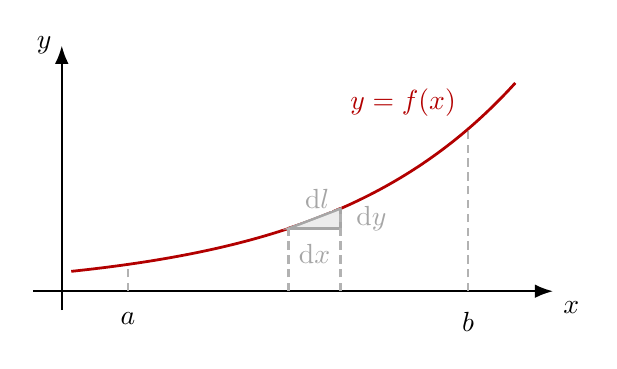
\begin{tikzpicture}[x=1.2cm,y=1.2cm,>=Latex,thick]
  % Axes
  \draw[-{Latex}] (-0.3,0) -- (5.2,0) node[below right] {$x$};
  \draw[-{Latex}] (0,-0.2) -- (0,2.6) node[left] {$y$};

  % Parameters
  % f(x) = 0.2 * exp(0.5 x)
  % Parameters
  \def\fa(#1){0.2*exp(0.5*(#1))}
% a and b
\def\xa{0.7}
\def\xb{4.3}
\pgfmathsetmacro{\ya}{\fa(\xa)}
\pgfmathsetmacro{\yb}{\fa(\xb)}

% Grey verticals at a and b (to the curve, not to 2.5)
\draw[densely dashed, gray!60] (\xa,0) -- (\xa,{\ya});
\draw[densely dashed, gray!60] (\xb,0) -- (\xb,{\yb});

% Labels a and b under the x-axis
\node[below=4pt] at (\xa,0) {$a$};
\node[below=4pt] at (\xb,0) {$b$};

% Curve
\draw[red!70!black, line width=1pt, domain=0.1:4.8, samples=160]
  plot (\x,{\fa(\x)});

% Label the function at (b, f(b))
\node[above left=1pt, red!70!black] at (\xb,{\fa(\xb)}) {$y=f(x)$};



  % Differential element around xm
  \def\xm{2.4}
  \def\dx{0.55}
  \pgfmathsetmacro{\xB}{\xm+\dx}
  \pgfmathsetmacro{\yA}{0.2*exp(0.5*\xm)}
  \pgfmathsetmacro{\yB}{0.2*exp(0.5*\xB)}

  % Small red arc segment on the curve (ds)
  \draw[red!70!black, line width=1.1pt, domain=\xm:\xB, samples=40]
    plot (\x,{\fa(\x)});

  % Right triangle (dx, dy, ds) in light grey
  % hypotenuse from (xm,yA) to (xB,yB)
  \path[fill=gray!15, draw=gray!60]
    (\xm,\yA) -- (\xB,\yA) -- (\xB,\yB) -- cycle;

  % Edges of triangle & labels
  \draw[gray!70] (\xm,\yA) -- (\xB,\yA) node[midway, below=2pt] {$\mathrm{d}x$};
  \draw[gray!70] (\xB,\yA) -- (\xB,\yB) node[midway, right=2pt] {$\mathrm{d}y$};
  \draw[gray!70] (\xm,\yA) -- (\xB,\yB)
        node[pos=0.55, above=2pt, fill=white, inner sep=1pt] {$\mathrm{d}l$};

  % Light construction lines for the element
  \draw[densely dashed, gray!60] (\xm,0) -- (\xm,{\yA});
  \draw[densely dashed, gray!60] (\xB,0) -- (\xB,{\yB});
\end{tikzpicture}

\end{minipage}
\\[0.8em]
% ===================== Row 4 =====================
\noindent
\begin{minipage}[c]{\linewidth}
\textbf{Polaire booglengte}\par
Voor een kromme $r=r(\theta)$, $\theta\in[\alpha,\beta]$:
\[
L=\int_{\alpha}^{\beta}\sqrt{r^2+\left(\frac{dr}{d\theta}\right)^{\!2}}\,d\theta.
\]
\end{minipage}\hfill
&
\begin{minipage}[r]{\linewidth}
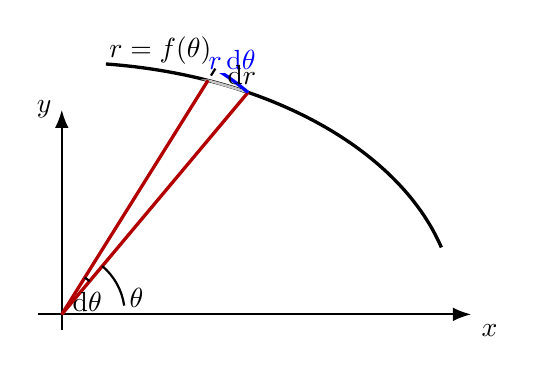
\begin{tikzpicture}[scale=1,>=Latex,thick]
  % axes
  \draw[-{Latex}] (-0.3,0) -- (5.2,0) node[below right] {$x$};
  \draw[-{Latex}] (0,-0.2) -- (0,2.6) node[left] {$y$};

  % ellipse parameters (semi-axes a on x, b on y)
  \def\a{5.0}
  \def\b{3.2}

  % main display angles
  \pgfmathsetmacro{\thetaplotA}{10}
  \pgfmathsetmacro{\thetaplotB}{80}

  % helper: r(θ) for the ellipse in polar form (origin at center)
  % r(θ) = ab / sqrt((b cosθ)^2 + (a sinθ)^2)
  % (We’ll inline this expression in plots)

  % highlight the ellipse arc between 10° and 80° (polar-by-angle)
  \draw[line width=1.2pt, black]
    plot[domain=\thetaplotA:\thetaplotB, samples=280, variable=\t]
      ({(\a*\b)/sqrt((\b*cos(\t))^2+(\a*sin(\t))^2)*cos(\t)},
       {(\a*\b)/sqrt((\b*cos(\t))^2+(\a*sin(\t))^2)*sin(\t)});

  % choose a local theta and dtheta for the differential element
  \pgfmathsetmacro{\th}{50}
  \pgfmathsetmacro{\dth}{8}

  % compute r(θ) and r(θ+dθ)
  \pgfmathsetmacro{\rth}{(\a*\b)/sqrt((\b*cos(\th))^2+(\a*sin(\th))^2)}
  \pgfmathsetmacro{\rthp}{(\a*\b)/sqrt((\b*cos(\th+\dth))^2+(\a*sin(\th+\dth))^2)}

  % fill the small polar "slice" bounded by the ellipse between θ and θ+dθ
  \path[fill=gray!12, draw=gray!45]
    (0,0) --
    (\th:\rth)
    plot[domain=\th:\th+\dth, samples=80, variable=\t]
      ({(\a*\b)/sqrt((\b*cos(\t))^2+(\a*sin(\t))^2)*cos(\t)},
       {(\a*\b)/sqrt((\b*cos(\t))^2+(\a*sin(\t))^2)*sin(\t)})
    -- (\th+\dth:\rthp) -- cycle;

  % the two rays
  \draw[very thick, red!70!black] (0,0) -- (\th:\rth);
  \draw[very thick, red!70!black] (0,0) -- (\th+\dth:\rthp);

  % circular arc at fixed radius r(θ): length ≈ r dθ
  \draw[very thick, blue]
    (\th:\rth) arc[start angle=\th, end angle=\th+\dth, radius=\rth]
    node[midway, above=2pt, fill=white, inner sep=1pt] {$r\,\mathrm d\theta$};

  % radial increment dr along the second ray
  \draw[densely dashed]
    (\th+\dth:\rth) -- (\th+\dth:\rthp)
    node[midway, right=2pt] {$\mathrm dr$};

  % angle markers and labels
  \draw (0.0,0) 
    ++(\th:0.55) arc (\th:\th+\dth:0.55)
      node[midway, below=1pt] {$\mathrm d\theta$};
  \draw (0,0) ++(8:0.8) arc (8:\th:0.8);
  \node at (0.95,0.21) {$\theta$};

  % annotate r = f(θ) near the arc
  \node[rotate=0] at
    ({(\a*\b)/sqrt((\b*cos(68))^2+(\a*sin(68))^2)*cos(68)},
     {(\a*\b)/sqrt((\b*cos(68))^2+(\a*sin(68))^2)*sin(68)+0.25})
     {$r=f(\theta)$};

  % small ticks at 10° and 80° rays for clarity
  \pgfmathsetmacro{\rmarkA}{(\a*\b)/sqrt((\b*cos(\thetaplotA))^2+(\a*sin(\thetaplotA))^2)}
  \pgfmathsetmacro{\rmarkB}{(\a*\b)/sqrt((\b*cos(\thetaplotB))^2+(\a*sin(\thetaplotB))^2)}


\end{tikzpicture}
\end{minipage}

\\
\end{tabular}


\newpage

%====================================================
% 3  COMBINATIELEER
%====================================================
\section{Combinatieleer}

\subsection{Keuzes zonder herhaling}

\begin{tabular}{|p{0.31\linewidth}|p{0.31\linewidth}|p{0.33\linewidth}|}
\hline
\textbf{Variaties} & \textbf{Permutaties} & \textbf{Combinaties} \\ \hline

\textbf{geordende keuze} \newline
(\textit{volgorde van belang}) \newline
van $p$ verschillende elementen \newline
uit $n$ elementen &
\textbf{Rangschikken} \newline
(\textit{volgorde van belang}) \newline
van $n$ verschillende elementen &
\textbf{ongeordende keuze} \newline
(\textit{volgorde van geen belang}) \newline
van $p$ verschillende elementen \newline
uit $n$ elementen \\ \hline

\[
V_n^p = \frac{n!}{(n-p)!}
\] 
&
\[{P_n} = V_n^n = \frac{{n!}}{{(n - n)!}} = n!\] &
\[C_n^p = \frac{{V_n^p}}{{P_p^{}}} = \frac{{\frac{{n!}}{{\left( {n - p} \right)!}}}}{{p!}} = \frac{{n!}}{{\left( {n - p} \right)!p!}}\] \\ \hline

\textit{Internationale notatie:} \newline
\[
V_n^p = {}_nP_p = P(n,p)
\] &
\textit{Internationale notatie:} \newline
\[
P_n = {}_nP_n = P(n) = n!
\] &
\textit{Internationale notatie:} \newline
\[
C_n^p = C(n,p) = \binom{n}{p}
\] \\ \hline

\end{tabular}

% ============================================================
\subsection{Keuzes met herhaling}

\begin{tabular}{|p{0.31\linewidth}|p{0.32\linewidth}|p{0.32\linewidth}|}
\hline
\textbf{Variaties met herhaling} &
\textbf{Permutaties met herhaling} &
\textbf{Combinaties met herhaling} \\ \hline

\textbf{geordende keuze} \newline
(\textit{volgorde van belang}) \newline
van $p$ elementen \newline
uit $n$ elementen \newline
\textit{(herhaling toegestaan)} &
\textbf{rangschikken van $n$ elementen} \newline
waarvan sommige \newline
\textit{identiek} zijn &
\textbf{ongeordende keuze} \newline
(\textit{volgorde van geen belang}) \newline
van $p$ elementen \newline
uit $n$ soorten elementen \newline
\textit{(herhaling toegestaan)} \\ \hline

\[
\overline{V}_n^p = n^p
\] &
\[\overline P _n^{m_1,m_2,\dotsm m_k} = \frac{{n!}}{{m_1!\,m_2!\,\dotsm m_k!}}\]

\smallskip

met $m_1 + \dotsb + m_k = n$ &
\[
\overline{C}_n^p
= C_{n+p-1}^p
= \frac{(n+p-1)!}{(n-1)!\,p!}
\] \\ \hline

\textit{Internationale notatie:} \newline
\[
\overline{V}_n^p = n^p
\] &
\textit{Internationale notatie:} \newline
 &
\textit{Internationale notatie:} \newline
\[
\overline{C}_n^p
= {}_nH_p
= \binom{n+p-1}{p}
\] \\ \hline

\end{tabular}

\newpage

\section{Statistiek}
Discrete data: slechts een eindig of telbaar aantal waarden is mogelijk.\\
Continue data: variabele die tussen twee waarden oneindig \# waarden kan aannemen.


% --------------------------------------------------------
% 1. Steekproef / Populatie / Normaalverdeling  (3x3 grid)
% --------------------------------------------------------
\noindent
\begin{tabular}{|p{0.30\linewidth}|p{0.30\linewidth}|p{0.31\linewidth}|}
\hline
\multicolumn{1}{|c|}{\textbf{Steekproef}} &
\multicolumn{1}{c|}{\textbf{Populatie}} &
\multicolumn{1}{c|}{\textbf{Normaalverdeling}} \\ \hline

$\displaystyle
\overline{x} = \frac{1}{n} \sum_{i=1}^{n} x_i
$ &
$\displaystyle
\mu = \frac{1}{N} \sum_{i=1}^{N} x_i
$ &
$\displaystyle
f(x) = \frac{1}{\sigma \sqrt{2\pi}} 
e^{-\frac{1}{2}\!\left(\frac{x - \mu}{\sigma}\right)^{\!2}}
$ \\[8pt]

$\displaystyle
s^2 = \frac{1}{n-1} \sum_{i=1}^{n} (x_i - \overline{x})^2
$ &
$\displaystyle
\sigma^2 = \frac{1}{N} \sum_{i=1}^{N} (x_i - \mu)^2
$ &
$N(\mu, \sigma)$ \\
\hline
\end{tabular}


% --------------------------------------------------------
% --------------------------------------------------------
% 2. Discrete en Continue (zelfde buitenbreedte)
% --------------------------------------------------------
{\scriptsize
\noindent
\begin{tabular}{|p{0.44\linewidth}|p{0.50\linewidth}|}
\hline
\multicolumn{1}{|c|}{\textbf{Discrete}} &
\multicolumn{1}{c|}{\textbf{Continue}} \\ \hline

\(\begin{aligned}
E[X] &= \mu_X = \sum_{i=1}^{n} X_i\!\cdot\!p_i \\[4pt]
\sigma_X^2 &= \sum_{i=1}^{n} (x_i - \mu_X)^2\!\cdot\!p_i \\[2pt]
&= \left(\sum_{i=1}^{n} x_i^2\!\cdot\!p_i \right) - \mu_X^2
\end{aligned}\)
&
\(\begin{aligned}
E[X] &= \mu_X = \int_a^b x\!\cdot\!f(x)\,dx \\[4pt]
\sigma_X^2 &= \int_a^b (x - \mu_X)^2\!\cdot\!f(x)\,dx \\[2pt]
&= \int_a^b x^2\!\cdot\!f(x)\,dx - \mu_X^2
\end{aligned}\)
\\
\hline
\end{tabular}
\normalsize
}


% 3. Rekenregels (zelfde buitenbreedte)
\noindent
\begin{tabular}{|p{0.30\linewidth}|p{0.30\linewidth}|p{0.31\linewidth}|}
\hline
\multicolumn{3}{|l|}{\textbf{Rekenregels}} \\ \hline
$T = X + a$ & $T = aX$ & $T = aX + bY$ \\[2pt]
$\mu_T = \mu_X + a$ & $\mu_T = a\!\cdot\!\mu_X$ & $\mu_T = a\mu_X + b\mu_Y$ \\[2pt]
$\sigma_T = \sigma_X$ & $\sigma_T = |a|\!\cdot\!\sigma_X$ & $\sigma_T = \sqrt{a^2\!\cdot\!\sigma_X^2 + b^2\!\cdot\!\sigma_Y^2}$ \\
\hline
\end{tabular}

\noindent
\small
\begin{tabular}{|p{0.28\linewidth}|p{0.68\linewidth}|}
\hline
\multicolumn{2}{|l|}{\textbf{Rekenregels}} \\ \hline
% --- Left column: somformules ---
\(\begin{aligned}
S &= X_1 + \dots + X_n \\[3pt]
\mu_S &= E(S) = n\mu_X \\[3pt]
\sigma_S^2 &= n\sigma_X^2 
\;\Rightarrow\;
\sigma_S = \sqrt{n}\!\cdot\!\sigma_X
\end{aligned}\)
&
% --- Right column: gemiddelde en CLT ---
\(\begin{aligned}
\left. {\begin{array}{*{20}{c}}
{\overline X  = \frac{{\left( {{X_1} + ... + {X_n}} \right)}}{n}\quad ,\quad {\mu _{\overline X }} = \frac{1}{n}n{\mu _X}}\\
{{\sigma _{_{\overline X }}}^2 = \frac{1}{{{n^2}}}n{\sigma _X}^2 = \frac{1}{n}{\sigma _X}^2 \Rightarrow {\sigma _{_{\overline X }}} = \frac{{{\sigma _X}}}{{\sqrt n }}}
\end{array}} \right\}\!CLT \!\to\! \overline X  \!\approx\! N({\mu _{\overline X }},\frac{{{\sigma _X}}}{{\sqrt n }})
\end{aligned}\)
\\
\hline
\end{tabular}
\normalsize



% 4. Uniforme, Bernoulli, Binomiaal (zelfde buitenbreedte)
\noindent
\begin{tabular}{|p{0.44\linewidth}|p{0.50\linewidth}|}
\hline
\textbf{Uniforme continue} &
\textbf{Uniforme discrete} \\ \hline
$\begin{aligned}
\mu &= \frac{a+b}{2} \\
\sigma &= \frac{b-a}{2\sqrt{3}}
\end{aligned}$ &
$\begin{aligned}
\mu &= \frac{1}{n} \sum_{i=1}^{n} x_i \\
\sigma^2 &= \frac{1}{n} \sum_{i=1}^{n} (x_i - \mu)^2 \\
&= \frac{1}{n} \sum_{i=1}^{n} (x_i^2) - \mu^2
\end{aligned}$ \\
\hline
\end{tabular}

\noindent
\begin{tabular}{|p{0.30\linewidth}|p{0.64\linewidth}|}
\hline
\textbf{Bernoulli} &
\textbf{Binomiaal} \\ \hline
\(\begin{aligned}
\mu &= p \\[2pt]
\sigma &= \sqrt{p\!\cdot\!q}
\end{aligned}\) 
&
\(\begin{aligned}
P(X = i) = C_i^n \cdot {p^i} \cdot {(1 - p)^{n - i}} \\[6pt]
\left\{
\begin{array}{l}
n \ge 20,\\
n\,p \ge 5 \;\wedge\; n\,q \ge 5
\end{array}
\right.
&\Rightarrow B(n,p) \approx N(n p,\sqrt{n p q})
\end{aligned}\) \\[2pt]
\hline
\end{tabular}

\newpage

\subsection{Standaardnormale verdeling}
\label{sec:ztable}

\begin{center}
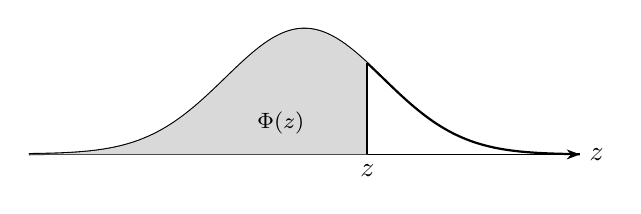
\begin{tikzpicture}[>=Stealth, scale=1]
  % x-as
  \draw[->] (-3.5,0) -- (3.5,0) node[right] {$z$};

  % normale kromme
  \draw[thick]
    plot[domain=-3.5:3.5,samples=200]
      (\x,{4/sqrt(2*pi)*exp(-\x*\x/2)});

  % voorbeeld-z
  \def\z{0.8}
  \fill[gray!30]
    plot[domain=-3.5:\z,samples=200]
      (\x,{4/sqrt(2*pi)*exp(-\x*\x/2)})
    -- (\z,0) -- (-3.5,0) -- cycle;

  \draw[thick] (\z,0) -- (\z,{4/sqrt(2*pi)*exp(-\z*\z/2)});
  \node[below] at (\z,0) {$z$};

  \node[align=left] at (-0.3,0.4) {\footnotesize $\Phi(z)$};
\end{tikzpicture}
\end{center}

\noindent
\[
\Phi(z)=\Pr(Z\le z)\quad\text{voor}\quad Z\sim\mathcal N(0,1).
\]
De rij geeft het eerste decimaal, de kolomkop het tweede decimaal.

\subsection*{Z-tabel}

\begin{center}
\setlength{\tabcolsep}{3pt}
\renewcommand{\arraystretch}{1.05}

\begingroup
\rowcolors{2}{gray!15}{white} % <-- light gray visible even when printed

\begin{tabular}{c|cccccccccc}
\toprule
$z$ & .00 & .01 & .02 & .03 & .04 & .05 & .06 & .07 & .08 & .09\\
\midrule
0.0 & 0.5000 & 0.5040 & 0.5080 & 0.5120 & 0.5160 & 0.5199 & 0.5239 & 0.5279 & 0.5319 & 0.5359 \\
0.1 & 0.5398 & 0.5438 & 0.5478 & 0.5517 & 0.5557 & 0.5596 & 0.5636 & 0.5675 & 0.5714 & 0.5753 \\
0.2 & 0.5793 & 0.5832 & 0.5871 & 0.5910 & 0.5948 & 0.5987 & 0.6026 & 0.6064 & 0.6103 & 0.6141 \\
0.3 & 0.6179 & 0.6217 & 0.6255 & 0.6293 & 0.6331 & 0.6368 & 0.6406 & 0.6443 & 0.6480 & 0.6517 \\
0.4 & 0.6554 & 0.6591 & 0.6628 & 0.6664 & 0.6700 & 0.6736 & 0.6772 & 0.6808 & 0.6844 & 0.6879 \\
0.5 & 0.6915 & 0.6950 & 0.6985 & 0.7019 & 0.7054 & 0.7088 & 0.7123 & 0.7157 & 0.7190 & 0.7224 \\
0.6 & 0.7257 & 0.7291 & 0.7324 & 0.7357 & 0.7389 & 0.7422 & 0.7454 & 0.7486 & 0.7517 & 0.7549 \\
0.7 & 0.7580 & 0.7611 & 0.7642 & 0.7673 & 0.7704 & 0.7734 & 0.7764 & 0.7794 & 0.7823 & 0.7852 \\
0.8 & 0.7881 & 0.7910 & 0.7939 & 0.7967 & 0.7995 & 0.8023 & 0.8051 & 0.8078 & 0.8106 & 0.8133 \\
0.9 & 0.8159 & 0.8186 & 0.8212 & 0.8238 & 0.8264 & 0.8289 & 0.8315 & 0.8340 & 0.8365 & 0.8389 \\
1.0 & 0.8413 & 0.8438 & 0.8461 & 0.8485 & 0.8508 & 0.8531 & 0.8554 & 0.8577 & 0.8599 & 0.8621 \\
1.1 & 0.8643 & 0.8665 & 0.8686 & 0.8708 & 0.8729 & 0.8749 & 0.8770 & 0.8790 & 0.8810 & 0.8830 \\
1.2 & 0.8849 & 0.8869 & 0.8888 & 0.8907 & 0.8925 & 0.8944 & 0.8962 & 0.8980 & 0.8997 & 0.9015 \\
1.3 & 0.9032 & 0.9049 & 0.9066 & 0.9082 & 0.9099 & 0.9115 & 0.9131 & 0.9147 & 0.9162 & 0.9177 \\
1.4 & 0.9192 & 0.9207 & 0.9222 & 0.9236 & 0.9251 & 0.9265 & 0.9279 & 0.9292 & 0.9306 & 0.9319 \\
1.5 & 0.9332 & 0.9345 & 0.9357 & 0.9370 & 0.9382 & 0.9394 & 0.9406 & 0.9418 & 0.9429 & 0.9441 \\
1.6 & 0.9452 & 0.9463 & 0.9474 & 0.9484 & 0.9495 & 0.9505 & 0.9515 & 0.9525 & 0.9535 & 0.9545 \\
1.7 & 0.9554 & 0.9564 & 0.9573 & 0.9582 & 0.9591 & 0.9599 & 0.9608 & 0.9616 & 0.9625 & 0.9633 \\
1.8 & 0.9641 & 0.9649 & 0.9656 & 0.9664 & 0.9671 & 0.9678 & 0.9686 & 0.9693 & 0.9699 & 0.9706 \\
1.9 & 0.9713 & 0.9719 & 0.9726 & 0.9732 & 0.9738 & 0.9744 & 0.9750 & 0.9756 & 0.9761 & 0.9767 \\
2.0 & 0.9772 & 0.9778 & 0.9783 & 0.9788 & 0.9793 & 0.9798 & 0.9803 & 0.9808 & 0.9812 & 0.9817 \\
2.1 & 0.9821 & 0.9826 & 0.9830 & 0.9834 & 0.9838 & 0.9842 & 0.9846 & 0.9850 & 0.9854 & 0.9857 \\
2.2 & 0.9861 & 0.9864 & 0.9868 & 0.9871 & 0.9875 & 0.9878 & 0.9881 & 0.9884 & 0.9887 & 0.9890 \\
2.3 & 0.9893 & 0.9896 & 0.9898 & 0.9901 & 0.9904 & 0.9906 & 0.9909 & 0.9911 & 0.9913 & 0.9916 \\
2.4 & 0.9918 & 0.9920 & 0.9922 & 0.9925 & 0.9927 & 0.9929 & 0.9931 & 0.9932 & 0.9934 & 0.9936 \\
2.5 & 0.9938 & 0.9940 & 0.9941 & 0.9943 & 0.9945 & 0.9946 & 0.9948 & 0.9949 & 0.9951 & 0.9952 \\
2.6 & 0.9953 & 0.9955 & 0.9956 & 0.9957 & 0.9959 & 0.9960 & 0.9961 & 0.9962 & 0.9963 & 0.9964 \\
2.7 & 0.9965 & 0.9966 & 0.9967 & 0.9968 & 0.9969 & 0.9970 & 0.9971 & 0.9972 & 0.9973 & 0.9974 \\
2.8 & 0.9974 & 0.9975 & 0.9976 & 0.9977 & 0.9977 & 0.9978 & 0.9979 & 0.9979 & 0.9980 & 0.9981 \\
2.9 & 0.9981 & 0.9982 & 0.9982 & 0.9983 & 0.9984 & 0.9984 & 0.9985 & 0.9985 & 0.9986 & 0.9986 \\
3.0 & 0.9987 & 0.9987 & 0.9987 & 0.9988 & 0.9988 & 0.9989 & 0.9989 & 0.9989 & 0.9990 & 0.9990 \\
3.1 & 0.9990 & 0.9991 & 0.9991 & 0.9991 & 0.9992 & 0.9992 & 0.9992 & 0.9992 & 0.9993 & 0.9993 \\
3.2 & 0.9993 & 0.9993 & 0.9994 & 0.9994 & 0.9994 & 0.9994 & 0.9994 & 0.9995 & 0.9995 & 0.9995 \\
3.3 & 0.9995 & 0.9995 & 0.9995 & 0.9996 & 0.9996 & 0.9996 & 0.9996 & 0.9996 & 0.9996 & 0.9997 \\
3.4 & 0.9997 & 0.9997 & 0.9997 & 0.9997 & 0.9997 & 0.9997 & 0.9997 & 0.9997 & 0.9997 & 0.9998 \\
\bottomrule
\end{tabular}
\endgroup
\end{center}

\newpage

\subsection{Schatters, betrouwbaarheidsintervallen}

\begin{flushleft}
\begin{tabular}{|p{0.22\linewidth}|p{0.38\linewidth}|p{0.38\linewidth}|}
\hline
\textbf{Puntschatting} & \textbf{Populatieparameter} & \textbf{Schatter uit de steekproef} \\
\hline
 & $p$ (proportie) & $\hat{p}$ \\
 & $\mu$ (gemiddelde) & $\bar{x}$ of $\hat{\mu}$ \\
 & $\sigma$ (standaardafwijking) & $s$ of $\hat{\sigma}$ \\
\hline
$\alpha\%$ - betrouwbaarheidsinterval &
Betrouwbaarheid $\alpha$ &
\begin{tabular}{c|ccccc}
 & 80\% & 90\% & 95\% & 98\% & 99\% \\ 
\hline
$z_\alpha$ & 1{,}28 & 1{,}65 & 1{,}96 & 2{,}33 & 2{,}58 \\
\end{tabular} \\
\hline
\textbf{Intervalschatting proportie} &
$\mu_{\hat{p}} = p, \quad \sigma_{\hat{p}} = \frac{1}{\sqrt{n}}\sqrt{pq}$ &
Betrouwbaarheidsinterval: $\hat{p} \pm z_\alpha \cdot \sigma_{\hat{p}}$ \\
\hline
\textbf{Intervalschatting normaalverdeling} &
 &
Betrouwbaarheidsinterval: $\bar{x} \pm z_\alpha \cdot \frac{\sigma}{\sqrt{n}}$ \\
\hline
\end{tabular}
\end{flushleft}

\subsection{Regressie}

\begin{flushleft}
\begin{tabular}{|p{0.44\linewidth}|p{0.50\linewidth}|}
\hline
\textbf{Regressielijn} &
$a = \dfrac{\sum_{i=1}^{n} (x_i - \bar{x})(y_i - \bar{y})}{\sum_{i=1}^{n} (x_i - \bar{x})^2} 
= \dfrac{S_{XY}^2}{S_X^2}, \quad
b = \bar{y} - a\bar{x}, \quad
y - \bar{y} = \dfrac{S_{XY}^2}{S_X^2}(x - \bar{x})$ \\
\hline
\textbf{Covariantie} &
$\mathrm{cov}(X,Y) = S_{XY}^2 = \dfrac{1}{n-1}\sum_{i=1}^{n}(x_i - \bar{x})(y_i - \bar{y})$ \\
\hline
\textbf{Correlatiecoëfficiënt} &
$r = \dfrac{S_{XY}^2}{S_X S_Y}$ \\
\hline
\end{tabular}
\end{flushleft}

\subsection{Test van een hypothese over het gemiddelde van een normaalverdeling}

\begin{flushleft}
{Dit is een test van een steekproefgemiddelde $\bar{x}$ volgens steekproefgemiddeldeverdeling $X \approx \mathcal{N}({\mu _{\bar x}}, {\sigma _{\bar x}} ) \approx \mathcal{N}(\mu, \frac{\sigma}{\sqrt{n}}) $ in de populatie $\mathcal{N}(\mu, \sigma)$}. Gebruikmakend van significantieniveau $\alpha$.
\end{flushleft}

\begin{center}
\begin{tabular}{|c|c|c|}
\hline
\textbf{Twee-zijdige test} & \textbf{Links-zijdige test} & \textbf{Rechts-zijdige test} \\
\hline
$\begin{array}{l}
H_0 : \mu = \mu_0 \\
H_A : \mu \ne \mu_0
\end{array}$ &
$\begin{array}{l}
H_0 : \mu = \mu_0 \\
H_A : \mu < \mu_0
\end{array}$ &
$\begin{array}{l}
H_0 : \mu = \mu_0 \\
H_A : \mu > \mu_0
\end{array}$ \\
\hline

% TikZ-plots met α-labels
\begin{minipage}{4cm}
\vspace{2mm}
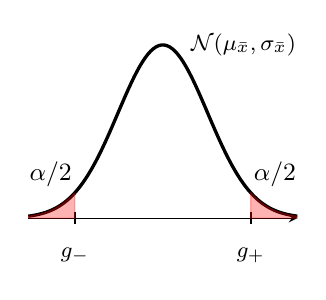
\begin{tikzpicture}
  \begin{axis}[
    axis x line=bottom,
    axis y line=none,
    domain=-3:3,
    samples=100,
    ymin=0,
    width=5cm,
    height=4cm,
    x tick label style={yshift=-5pt},
    xtick style={color=black, thick},
    xtick={-1.96, 1.96},
    xticklabels={$g_{-}$, $g_{+}$},
    tick label style={font=\footnotesize}
  ]
    \addplot [very thick, black] {exp(-x^2/2)/sqrt(2*pi)};
    \addplot [red, domain=-3:-1.96, fill=red, opacity=0.3] {exp(-x^2/2)/sqrt(2*pi)} \closedcycle;
    \addplot [red, domain=1.96:3, fill=red, opacity=0.3] {exp(-x^2/2)/sqrt(2*pi)} \closedcycle;
    \node at (axis cs:-2.5,0.1) {\small $\alpha/2$};
    \node at (axis cs:2.5,0.1) {\small $\alpha/2$};
    \node at (axis cs:1.8,0.4) {\footnotesize $\mathcal{N}({\mu _{\bar x}}, {\sigma _{\bar x}} )$};
  \end{axis}
\end{tikzpicture}
\end{minipage}
&
\begin{minipage}{4cm}
\vspace{2mm}
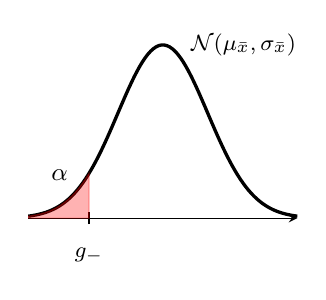
\begin{tikzpicture}
  \begin{axis}[
    axis x line=bottom,
    axis y line=none,
    domain=-3:3,
    samples=100,
    ymin=0,
    width=5cm,
    height=4cm,
    x tick label style={yshift=-5pt},
    xtick style={color=black, thick},
    xtick={-1.645},
    xticklabels={$g_{-}$},
    tick label style={font=\footnotesize}
  ]
    \addplot [very thick, black] {exp(-x^2/2)/sqrt(2*pi)};
    \addplot [red, domain=-3:-1.645, fill=red, opacity=0.3] {exp(-x^2/2)/sqrt(2*pi)} \closedcycle;
    \node at (axis cs:-2.3,0.1) {\small $\alpha$};
    \node at (axis cs:1.8,0.4) {\footnotesize $\mathcal{N}({\mu _{\bar x}}, {\sigma _{\bar x}} )$};
  \end{axis}
\end{tikzpicture}
\end{minipage}
&
\begin{minipage}{4cm}
\vspace{2mm}
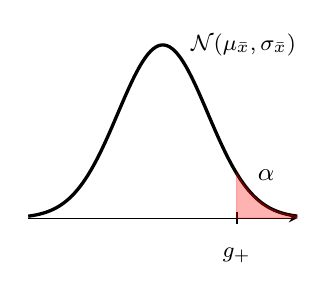
\begin{tikzpicture}
  \begin{axis}[
    axis x line=bottom,
    axis y line=none,
    domain=-3:3,
    samples=100,
    ymin=0,
    width=5cm,
    height=4cm,
    x tick label style={yshift=-5pt},
    xtick style={color=black, thick},
    xtick={1.645},
    xticklabels={$g_{+}$},
    tick label style={font=\footnotesize}
  ]
    \addplot [very thick, black] {exp(-x^2/2)/sqrt(2*pi)};
    \addplot [red, domain=1.645:3, fill=red, opacity=0.3] {exp(-x^2/2)/sqrt(2*pi)} \closedcycle;
    \node at (axis cs:2.3,0.1) {\small $\alpha$};
    \node at (axis cs:1.8,0.4) {\footnotesize $\mathcal{N}({\mu _{\bar x}}, {\sigma _{\bar x}} )$};
  \end{axis}
\end{tikzpicture}
\end{minipage}
\\
\hline
$\displaystyle H_A : {z _{\bar x}} \le g_{-} \,\, \vee \,\, \bar{x} \ge g_{+}$ &
$\displaystyle H_A : {z _{\bar x}} \le g_{-}$ &
$\displaystyle H_A : {z _{\bar x}} \ge g_{+}$ \\
\hline
\end{tabular}
\end{center}

\subsection{Test van een hypothese over een populatieproportie}

\begin{flushleft}
{Dit is een test op een populatieproportie $\hat{p}$ volgens een binomiaalverdeling $X \approx \mathcal{B}(n,p) \approx \mathcal{N}(np,{\sqrt{n}} . {\sqrt{p(1-p)}})$}. Gebruikmakend van significantieniveau $\alpha$.
\end{flushleft}

\begin{center}
\begin{tabular}{|c|c|c|}
\hline
\textbf{Twee-zijdige test} & \textbf{Links-zijdige test} & \textbf{Rechts-zijdige test} \\
\hline
$\begin{array}{l}
H_0 : p = p_0 \\
H_A : p \ne p_0
\end{array}$ &
$\begin{array}{l}
H_0 : p = p_0 \\
H_A : p < p_0
\end{array}$ &
$\begin{array}{l}
H_0 : p = p_0 \\
H_A : p > p_0
\end{array}$ \\
\hline

% TikZ-plots voor proportietoets
\begin{minipage}{4cm}
\vspace{2mm}
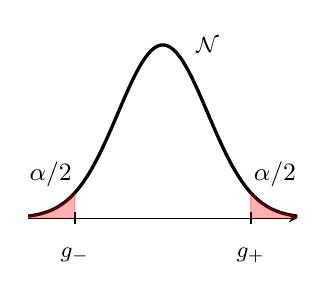
\begin{tikzpicture}
  \begin{axis}[
    axis x line=bottom,
    axis y line=none,
    domain=-3:3,
    samples=100,
    ymin=0,
    width=5cm,
    height=4cm,
    x tick label style={yshift=-5pt},
    xtick style={color=black, thick},
    xtick={-1.96, 1.96},
    xticklabels={$g_{-}$, $g_{+}$},
    tick label style={font=\footnotesize}
  ]
    \addplot [very thick, black] {exp(-x^2/2)/sqrt(2*pi)};
    \addplot [red, domain=-3:-1.96, fill=red, opacity=0.3] {exp(-x^2/2)/sqrt(2*pi)} \closedcycle;
    \addplot [red, domain=1.96:3, fill=red, opacity=0.3] {exp(-x^2/2)/sqrt(2*pi)} \closedcycle;
    \node at (axis cs:-2.5,0.1) {\small $\alpha/2$};
    \node at (axis cs:2.5,0.1) {\small $\alpha/2$};
    \node at (axis cs:1,0.4) {\footnotesize $\mathcal{N}$};
  \end{axis}
\end{tikzpicture}
\end{minipage}
&
\begin{minipage}{4cm}
\vspace{2mm}
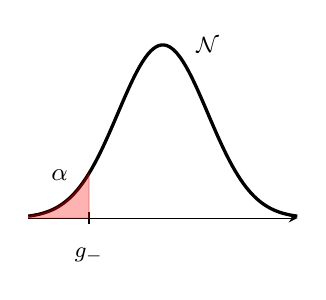
\begin{tikzpicture}
  \begin{axis}[
    axis x line=bottom,
    axis y line=none,
    domain=-3:3,
    samples=100,
    ymin=0,
    width=5cm,
    height=4cm,
    x tick label style={yshift=-5pt},
    xtick style={color=black, thick},
    xtick={-1.645},
    xticklabels={$g_{-}$},
    tick label style={font=\footnotesize}
  ]
    \addplot [very thick, black] {exp(-x^2/2)/sqrt(2*pi)};
    \addplot [red, domain=-3:-1.645, fill=red, opacity=0.3] {exp(-x^2/2)/sqrt(2*pi)} \closedcycle;
    \node at (axis cs:-2.3,0.1) {\small $\alpha$};
    \node at (axis cs:1,0.4) {\footnotesize $\mathcal{N}$};
  \end{axis}
\end{tikzpicture}
\end{minipage}
&
\begin{minipage}{4cm}
\vspace{2mm}
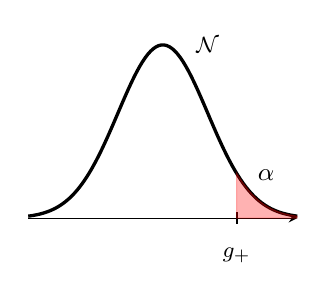
\begin{tikzpicture}
  \begin{axis}[
    axis x line=bottom,
    axis y line=none,
    domain=-3:3,
    samples=100,
    ymin=0,
    width=5cm,
    height=4cm,
    x tick label style={yshift=-5pt},
    xtick style={color=black, thick},
    xtick={1.645},
    xticklabels={$g_{+}$},
    tick label style={font=\footnotesize}
  ]
    \addplot [very thick, black] {exp(-x^2/2)/sqrt(2*pi)};
    \addplot [red, domain=1.645:3, fill=red, opacity=0.3] {exp(-x^2/2)/sqrt(2*pi)} \closedcycle;
    \node at (axis cs:2.3,0.1) {\small $\alpha$};
    \node at (axis cs:1,0.4) {\footnotesize $\mathcal{N}$};
  \end{axis}
\end{tikzpicture}
\end{minipage}
\\
\hline
$\displaystyle H_A : \hat{p} \le g_{-} \,\, \vee \,\, \hat{p} \ge g_{+}$ &
$\displaystyle H_A : \hat{p} \le g_{-}$ &
$\displaystyle H_A : \hat{p} \ge g_{+}$ \\
\hline
\end{tabular}
\end{center}

\subsection{Test van een hypothese over het gemiddelde van een normaalverdeling via de P-waarde}

\begin{center}
\begin{tabular}{|p{4.8cm}|p{3.8cm}|p{4cm}|}
\hline
\textbf{Twee-zijdige toets} & \textbf{Links éénzijdige toets} & \textbf{Rechts éénzijdige toets} \\
\hline
\begin{tabular}{@{}l@{}}
$H_0: \mu = \mu_0$ \\
$H_1: \mu \ne \mu_0$
\end{tabular}
&
\begin{tabular}{@{}l@{}}
$H_0: \mu = \mu_0$ \\
$H_1: \mu < \mu_0$
\end{tabular}
&
\begin{tabular}{@{}l@{}}
$H_0: \mu = \mu_0$ \\
$H_1: \mu > \mu_0$
\end{tabular}
\\
\hline
\begin{tabular}{@{}l@{}}
Als $\bar{x} < \mu$ $\rightarrow$ $P = 2 \cdot P(X \leq \bar{x})$ \\
Als $\bar{x} > \mu$ $\rightarrow$ $P = 2 \cdot P(X \geq \bar{x})$
\end{tabular}
&
$P = P(X \leq \bar{x})$
&
$P = P(X \geq \bar{x})$ \\
\hline
$P \leq \alpha$ & $P \leq \alpha$ & $P \leq \alpha$ \\
\hline
\end{tabular}
\end{center}


\subsection{Test van een hypothese over een populatieproportie via de P-waarde}

\begin{center}
\begin{tabular}{|p{4.8cm}|p{3.8cm}|p{4cm}|}
\hline
\textbf{Twee-zijdige toets} & \textbf{Linkszijdige toets} & \textbf{Rechtszijdige toets} \\
\hline
\begin{tabular}{@{}l@{}}
$H_0: p = p_0$ \\
$H_1: p \ne p_0$
\end{tabular}
&
\begin{tabular}{@{}l@{}}
$H_0: p = p_0$ \\
$H_1: p < p_0$
\end{tabular}
&
\begin{tabular}{@{}l@{}}
$H_0: p = p_0$ \\
$H_1: p > p_0$
\end{tabular}
\\
\hline
\begin{tabular}{@{}l@{}}
Als $\hat{p} < p$ $\rightarrow$ $P = 2 \cdot P(X \leq \hat{p})$ \\
Als $\hat{p} > p$ $\rightarrow$ $P = 2 \cdot P(X \geq \hat{p})$
\end{tabular}
&
$P = P(X \leq \hat{p})$
&
$P = P(X \geq \hat{p})$ \\
\hline
Vergelijk: $P \leq \alpha$ & Vergelijk: $P \leq \alpha$ & Vergelijk: $P \leq \alpha$ \\
\hline
\end{tabular}
\end{center}

\section{Kans}

% ---------------------------------------------------
% Kansrekenen – overzichtstabel (één tabular)
% ---------------------------------------------------
\renewcommand{\arraystretch}{1.2}

\begin{tabular}{|p{0.48\linewidth}|p{0.48\linewidth}|}
\hline
\multicolumn{2}{|c|}{\textbf{Willekeurige en onafhankelijke gebeurtenissen}} \\ \hline
\textbf{Willekeurig} & \textbf{Onafhankelijk} \\ \hline
\begin{center}
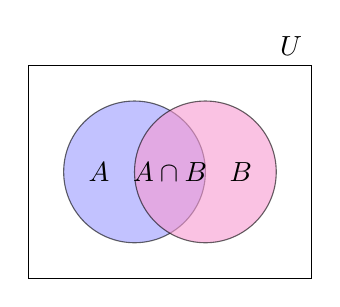
\begin{tikzpicture}[scale=0.9]
  \draw (-1.5,-1.5) rectangle (2.5,1.5) node[above left] {$U$};
  \draw[fill=blue!40,opacity=0.6] (0,0) circle (1);
  \draw[fill=magenta!40,opacity=0.6] (1,0) circle (1);
  \node at (-0.5,0) {$A$};
  \node at (1.5,0) {$B$};
  \node at (0.5,0) {$A\cap B$};
\end{tikzpicture}
\end{center}
&
\begin{center}
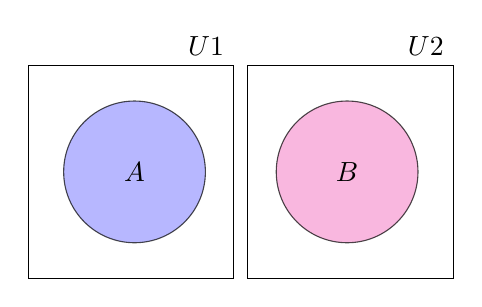
\begin{tikzpicture}[scale=0.9]
  \draw (-1.5,-1.5) rectangle (1.4,1.5) node[above left] {$U1$};
  \draw (1.6,-1.5) rectangle (4.5,1.5) node[above left] {$U2$};
  \draw[fill=blue!40,opacity=0.7] (0,0) circle (1);
  \node at (0,0) {$A$};
  \draw[fill=magenta!40,opacity=0.7] (3,0) circle (1);
  \node at (3,0) {$B$};
\end{tikzpicture}
\end{center}
\\[2pt]

$\begin{aligned}
P(A\setminus B) &= P(A)-P(A\cap B),\\[2pt]
P(A\cup B) &= P(A)+P(B)-P(A\cap B)
\end{aligned}$
&
$P(A\wedge B)=P(A)\cdot P(B)$
\\
\hline

\multicolumn{2}{|c|}{\textbf{Voorwaardelijke kans}} \\ \hline
$P(B\mid A)=\dfrac{P(B\cap A)}{P(A)}$ &
$P(B\mid A)=\dfrac{P(B\wedge A)}{P(A)}$ \\ \hline

\multicolumn{2}{|c|}{\textbf{Productwet}} \\ \hline
$P(A\cap B)=P(A)\cdot P(B\mid A)$ &
$P(A\wedge B)=P(A)\cdot P(B\mid A)$ \\ \hline

\multicolumn{2}{|c|}{\textbf{Wet van de totale kans}} \\ \hline
\textbf{Willekeurig} & \textbf{Onafhankelijk} \\ \hline

\begin{center}
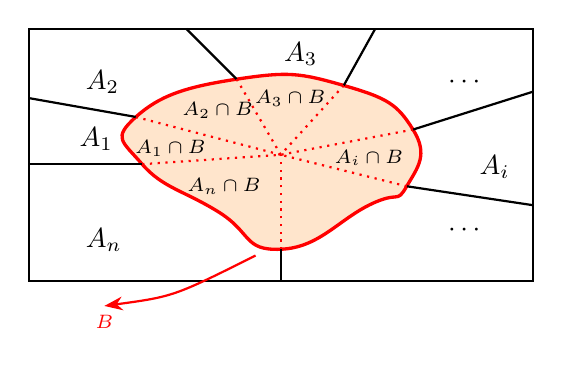
\begin{tikzpicture}[scale=0.8,>=Stealth]

% Center of B
\coordinate (C) at (0,0);

%------------------------
% Universe U
%------------------------
\draw[thick] (-4,-2) rectangle (4,2);

%------------------------
% Points on the rays where they hit B
%------------------------
\def\Bpoints{
  (-2.3,0.6)   % A2
  (-2.2,-0.15) % A1 (slightly lower again)
  (-1.0,-0.9)
  (0,-1.5)     % A_n
  (1.4,-0.8)
  (2.0,-0.5)
  (2.1,0.4)
  (1.0,1.1)
  (-0.7,1.2)
}

%------------------------
% Set B: smooth red closed curve
%------------------------
\fill[orange!20]
  plot[smooth cycle, tension=0.9]
    coordinates {\Bpoints};

\draw[very thick,red]
  plot[smooth cycle, tension=0.9]
    coordinates {\Bpoints};

%------------------------
% Partition lines A_1,...,A_n
%------------------------
% A_1 (slightly lower)
\draw[thick] (-4,-0.15) -- (-2.2,-0.15);
\draw[thick,red,dotted] (-2.2,-0.15) -- (C);

% A_2
\draw[thick] (-4,0.9) -- (-2.3,0.6);
\draw[thick,red,dotted] (-2.3,0.6) -- (C);

% A_3
\draw[thick] (-1.5,2) -- (-0.7,1.2);
\draw[thick,red,dotted] (-0.7,1.2) -- (C);

% Next (upper right)
\draw[thick] (1.5,2) -- (1.0,1.1);
\draw[thick,red,dotted] (1.0,1.1) -- (C);

% A_i (right upper)
\draw[thick] (4,1.0) -- (2.1,0.4);
\draw[thick,red,dotted] (2.1,0.4) -- (C);

% lower right
\draw[thick] (4,-0.8) -- (2.0,-0.5);
\draw[thick,red,dotted] (2.0,-0.5) -- (C);

% A_n (bottom)
\draw[thick] (0,-2) -- (0,-1.5);
\draw[thick,red,dotted] (0,-1.5) -- (C);

%------------------------
% Labels for A_i regions (aligned)
%------------------------
\node[font=\normalsize,anchor=west] at (-3.35,0.25) {$A_1$};
\node[font=\normalsize,anchor=west] at (-3.25,1.15) {$A_2$};
\node[font=\normalsize,anchor=west] at (-0.1,1.6) {$A_3$};
\node[font=\normalsize,anchor=west] at (2.5,1.15) {$\cdots$};
\node[font=\normalsize,anchor=west] at (3.0,-0.2) {$A_{i}$};
\node[font=\normalsize,anchor=west] at (2.5,-1.2)
{$\cdots$};
\node[font=\normalsize,anchor=west] at (-3.25,-1.35) {$A_n$};

%------------------------
% Labels inside B: A_i ∩ B
%------------------------
\node[font=\scriptsize] at (-1.75,0.1) {$A_1\cap B$};
\node[font=\scriptsize] at (-1,0.7) {$A_2\cap B$};
\node[font=\scriptsize] at (0.15,0.9) {$A_3\cap B$};
\node[font=\scriptsize] at (1.4,-0.05) {$A_i\cap B$};
\node[font=\scriptsize] at (-0.9,-0.5) {$A_n\cap B$};

%------------------------
% Arrow + label B (lower & left)
%------------------------
\draw[red,->,thick]
  (-0.4,-1.6) .. controls (-1.7,-2.25) .. (-2.8,-2.4);
\node[red,below,font=\scriptsize] at (-2.8,-2.4) {$B$};

\end{tikzpicture}

\end{center}
&
%======================
% picture onafhankeljk
%======================
\begin{center}
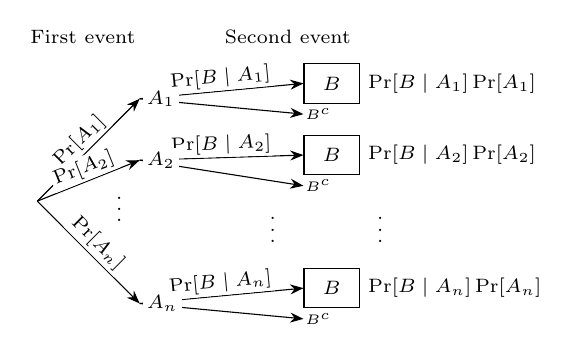
\begin{tikzpicture}[
    >=Stealth,
    every node/.style={font=\scriptsize},
    scale=0.65
]

%======================
% Coordinates
%======================

\coordinate (O)  at (-3.7,0);

\coordinate (A1) at (-1.7, 2.0);
\coordinate (A2) at (-1.7, 0.8);
\coordinate (An) at (-1.7,-2.0);

\def\BX{1.5}

\coordinate (A1B)  at (\BX, 2.3);
\coordinate (A1Bc) at (\BX, 1.7);
\coordinate (A2B)  at (\BX, 0.9);
\coordinate (A2Bc) at (\BX, 0.3);
\coordinate (AnB)  at (\BX,-1.7);
\coordinate (AnBc) at (\BX,-2.3);

%======================
% Arrows
%======================

% First event
\draw[->] (O) -- (A1)
    node[midway, above, sloped, fill=white, inner sep=1pt] {$\Pr[A_1]$};
\draw[->] (O) -- (A2)
    node[midway, above, sloped, fill=white, inner sep=1pt] {$\Pr[A_2]$};
\draw[->] (O) -- (An)
    node[midway, above, sloped, fill=white, inner sep=1pt] {$\Pr[A_n]$};

% Second event from A1
\draw[->] (A1) -- (A1B)
    node[midway, above, sloped, fill=white, inner sep=1pt] {$\Pr[B\mid A_1]$};
\draw[->] (A1) -- (A1Bc);

% Second event from A2
\draw[->] (A2) -- (A2B)
    node[midway, above, sloped, fill=white, inner sep=1pt] {$\Pr[B\mid A_2]$};
\draw[->] (A2) -- (A2Bc);

% Second event from An
\draw[->] (An) -- (AnB)
    node[midway, above, sloped, fill=white, inner sep=1pt] {$\Pr[B\mid A_n]$};
\draw[->] (An) -- (AnBc);

%======================
% A_i labels (white background, slight shift)
%======================

\node[right=1pt, fill=white, inner sep=1.5pt] at (A1) {$A_1$};
\node[right=1pt, fill=white, inner sep=1.5pt] at (A2) {$A_2$};
\node[right=1pt, fill=white, inner sep=1.5pt] at (An) {$A_n$};

% Vertical dots
\node[fill=white, inner sep=1pt] at (-2.1,0.0) {$\vdots$};

%======================
% B boxes
%======================

\node[draw, rectangle, minimum width=7mm, minimum height=5mm,
      anchor=west, fill=white, inner sep=1pt] at (A1B) {$B$};
\node[draw, rectangle, minimum width=7mm, minimum height=5mm,
      anchor=west, fill=white, inner sep=1pt] at (A2B) {$B$};
\node[draw, rectangle, minimum width=7mm, minimum height=5mm,
      anchor=west, fill=white, inner sep=1pt] at (AnB) {$B$};

%======================
% B^c endpoints (like B, but smaller & no box)
%======================

\node[anchor=west, font=\tiny, fill=white, inner sep=0.5pt] at (A1Bc) {$B^{c}$};
\node[anchor=west, font=\tiny, fill=white, inner sep=0.5pt] at (A2Bc) {$B^{c}$};
\node[anchor=west, font=\tiny, fill=white, inner sep=0.5pt] at (AnBc) {$B^{c}$};

%======================
% Headers
%======================

\node[anchor=north west, fill=white, inner sep=1pt]
  at (-3.9,3.4) {First event};
\node[anchor=north west, fill=white, inner sep=1pt]
  at (-0.1,3.4) {Second event};

%======================
% Middle dots between branches
%======================

\node[fill=white, inner sep=1pt] at (0.9,-0.4) {$\vdots$};
\node[fill=white, inner sep=1pt] at (3.0,-0.4) {$\vdots$};

%======================
% Right-hand products
%======================

\node[anchor=west, fill=white, inner sep=1pt]
  at ($(A1B)+(1.2,0)$) {$\Pr[B\mid A_1]\Pr[A_1]$};
\node[anchor=west, fill=white, inner sep=1pt]
  at ($(A2B)+(1.2,0)$) {$\Pr[B\mid A_2]\Pr[A_2]$};
\node[anchor=west, fill=white, inner sep=1pt]
  at ($(AnB)+(1.2,0)$) {$\Pr[B\mid A_n]\Pr[A_n]$};

\end{tikzpicture}





\end{center}
\\[-2pt]
\multicolumn{2}{|c|}{$\displaystyle P(B) = \sum_{i=1}^{n} P(A_i)\cdot P(B\mid A_i)$} \\ \hline

\multicolumn{2}{|c|}{\textbf{Regel van Bayes}} \\ \hline
\multicolumn{2}{|c|}{$\displaystyle
P({A_i}|B) = \frac{{P({A_i} \wedge B)}}{{P(B)}} = \frac{{P({A_i}).P(B|{A_i})}}{{\sum\limits_{i = 1}^n {P({A_i}).P(B|{A_i})} }}
$} \\ \hline
\end{tabular}

\section{Diversen}
\subsection{Wiskundige symbolen (ISO 80000-2)}
% (ISO 31-11 werd vervangen door ISO 80000-2)

% ---- Typografische richtlijnen volgens ISO 80000-2 ----
% Variabelen cursief: a, b, x, f, ...
% Functienamen en vaste constanten recht (roman): \sin, \cos, \ln, \exp, \mathrm e, \mathrm i, \pi, \mathrm d
% Differentiëlen recht: \mathrm d x i.p.v. dx
% Voor logaritme grondtal 10: \lg x (i.p.v. \log x om ambiguïteit te vermijden)

\renewcommand{\arraystretch}{1.2}

% ------------------------------------------------------------
\subsubsection{Verzamelingen}

\begin{tabular}{>{$}l<{$} l}
\in & is een element van de verzameling \\
\notin & is geen element van de verzameling \\
\{a,b,c,\dots\} & verzameling door opsomming \\
\{x \mid p(x)\} & verzameling van $x$ met eigenschap $p(x)$ \\
\varnothing & de lege verzameling \\
\mathbb{N} & natuurlijke getallen $(0,1,2,\dots)$ \\
\mathbb{Z} & gehele getallen $(\dots,-2,-1,0,1,2,\dots)$ \\
\mathbb{Q} & rationale getallen (breuken van gehele getallen) \\
\mathbb{R} & reële getallen \\
\mathbb{C} & complexe getallen \\
B \subseteq A & $B$ is deelverzameling van $A$ (mag samenvallen) \\
B \subset A & $B$ is strikte deelverzameling van $A$ \\
A \cup B & unie van $A$ en $B$ \\
A \cap B & doorsnede van $A$ en $B$ \\
A \setminus B & verschil $A - B$ (in $A$ maar niet in $B$) \\
A^c \text{ of } \overline{A} & complement van $A$ in universum $U$ \\
(a,b) & geordend paar \\
(a_1,a_2,\dots,a_n) & geordend $n$-tal \\
A \times B & cartesisch product van $A$ en $B$ \\
\#A & aantal elementen (cardinaliteit) van $A$ \\
\end{tabular}

% ------------------------------------------------------------
\subsubsection{Logische symbolen}

\begin{tabular}{>{$}l<{$} l}
p \land q & conjunctie: $p$ en $q$ zijn beide waar \\
p \lor q & disjunctie: $p$ of $q$ is waar (of beide) \\
\lnot p & negatie: $p$ is niet waar \\
p \Rightarrow q & implicatie: als $p$, dan $q$ \\
p \Leftrightarrow q & equivalentie: $p$ en $q$ gelijkwaardig \\
\forall x & universele kwantor: voor alle $x$ \\
\exists x & existentiële kwantor: er bestaat (minstens één) $x$ \\
\end{tabular}

% ------------------------------------------------------------
\subsubsection{Diverse symbolen}

\begin{tabular}{>{$}l<{$} l}
a = b & $a$ is gelijk aan $b$ \\
a \ne b & $a$ is niet gelijk aan $b$ \\
a \coloneqq b & $a$ is per definitie gelijk aan $b$ \\
a \approx b & $a$ is bij benadering gelijk aan $b$ \\
a < b & $a$ is strikt kleiner dan $b$ \\
a > b & $a$ is strikt groter dan $b$ \\
a \le b & $a$ is kleiner of gelijk aan $b$ \\
a \ge b & $a$ is groter of gelijk aan $b$ \\
\infty & oneindig \\
\end{tabular}

% ------------------------------------------------------------
\subsubsection{Bewerkingen}

\begin{tabular}{E l}
a + b & optelling \\
a - b & aftrekking \\
a \cdot b,\; a \times b,\; a*b & vermenigvuldiging \\
\dfrac{a}{b},\; a/b & deling \\
a^p & $a$ tot de macht $p$ \\
\sqrt{a} , a^{\frac{1}{2}} & vierkantswortel uit $a$ \\
\sqrt[p]{a} , a^{\frac{1}{p}} & $p$-de machtswortel uit $a$ \\
\lvert a\rvert & absolute waarde van $a$ \\
\operatorname{sgn}(a) & signum van $a$: $(1$ als $a>0$, $0$ als $a=0$, $-1$ als $a<0)$ \\
\overline{a} & gemiddelde/verwachting (contextafhankelijk) \\
n! & $n$-faculteit; $n! = n(n-1)\dots 2\cdot 1$ \\
\binom{n}{k} & binomiaalcoëfficiënt $\displaystyle\binom{n}{k}=\frac{n!}{k!(n-k)!}$ \\
\lfloor a \rfloor & grootste geheel getal $\le a$ (vloer) \\
\sum_{i=1}^{n} a_i & som: $a_1 + a_2 + \dots + a_n$ \\
\prod_{i=1}^{n} a_i & product: $a_1 \cdot a_2 \cdot \dots \cdot a_n$
\end{tabular}


% ------------------------------------------------------------
\subsubsection{Functies \& analyse}

\begin{tabular}{>{$}l<{$} l}
f                             & functie $f$ \\
f(x)                          & functiewaarde \\
\left[f(x)\right]_a^b = f(b) - f(a)
                              & verschil gebruikt bij integralen \\
g \circ f                     & samengestelde functie: $g(f(x))$ \\
x \to a                       & $x$ streeft naar $a$ \\
\displaystyle \lim_{x \to a} f(x)
                              & limiet van $f(x)$ voor $x \to a$ \\
\Delta x                      & toename van $x$ \\
Df,\; f',\; \dfrac{\diff f}{\diff x}
                              & afgeleide van $f$ naar $x$ \\
Df(a),\; f'(a),\; \left.\dfrac{\diff f}{\diff x}\right|_{x=a}
                              & waarde van de afgeleide bij $x=a$ \\
\dfrac{d^{n}f}{dx^{n}},\; f^{(n)},\; D^{n}f
                              & $n$-de afgeleide van $f$ \\[8pt]
\displaystyle \frac{\pdiff f}{\pdiff x}
                              & partiële afgeleide van $f$ naar $x$ \\
\mathrm df                    & differentiaal van $f$: $\mathrm df = f'(x)\,\mathrm dx$ \\
\displaystyle \int f(x)\,\mathrm dx
                              & onbepaalde integraal (primitieven) \\
\displaystyle \int_a^b f(x)\,\mathrm dx
                              & bepaalde integraal over $[a,b]$ \\
\end{tabular}

% ------------------------------------------------------------
\subsubsection{Exponentiële en logaritmische functies}

\begin{tabular}{>{$}l<{$} l}
\mathrm e & basis van de natuurlijke logaritmen \\
\mathrm e^{x} & exponentiële functie met grondtal $\mathrm e$ \\
a^{x} & exponentiële functie met grondtal $a>0,\ a\ne 1$ \\
\log_a x & logaritme met grondtal $a$ \\
\ln x & natuurlijke logaritme van $x$ \\
\log_{10},\log,\lg x & decimale (Briggs) logaritme (grondtal $10$) \\
\end{tabular}

% ------------------------------------------------------------
\subsubsection{Goniometrische en hyperbolische functies}

\begin{tabular}{>{$}l<{$} l}
\pi & verhouding tussen omtrek en middellijn van een cirkel \\
\sin x,\ \cos x,\ \tan x,\ \cot x & sinus, cosinus, tangens, cotangens \\
\sec x = \dfrac{1}{\cos x},\ \csc x = \dfrac{1}{\sin x} & secans, cosecans \\
\arcsin x,\ \arccos x,\ \arctan x,\ \arccot x & inverse goniometrische functies \\
\arcsec x,\ \arccsc x & inverse secans en cosecans \\
\sinh x,\ \cosh x,\ \tanh x,\ \coth x & hyperbolische functies \\
\sech x,\ \csch x & hyperbolische secans, cosecans \\
\end{tabular}

% ------------------------------------------------------------
\subsubsection{Complexe getallen}

\begin{tabular}{>{$}l<{$} l}
\mathrm i,\ \mathrm j & imaginaire eenheid ($\mathrm i^2=-1$;\ $\mathrm j$ in elektronica) \\
z = a + b\,\mathrm i & complex getal $z$ \\
\Re z,\ \Im z & reëel respectievelijk imaginair deel van $z$ \\
\lvert z\rvert & modulus van $z$ \\
\arg z & argument van $z$ \\
z^\ast & geconjugeerd: $a - b\,\mathrm i$ \\
\end{tabular}


\subsection{Griekse alfabet}

\begin{center}
\renewcommand{\arraystretch}{1.1}
\setlength{\tabcolsep}{4pt} % compacte kolomafstand
\begin{tabular}{|
  >{\bfseries}c c l | % kolommen 1–3
  >{\bfseries}c c l | % kolommen 4–6
  >{\bfseries}c c l | % kolommen 7–9
  >{\bfseries}c c l | % kolommen 10–12
}
A & $\alpha$ & alfa &
$\Delta$ & $\delta$ & delta &
$\Theta$ & $\theta$ & thèta &
$\Lambda$ & $\lambda$ & lambda \\

B & $\beta$ & bèta &
E & $\varepsilon$ & epsilon &
I & $\iota$ & iota &
M & $\mu$ & mu \\

$\Gamma$ & $\gamma$ & gamma &
Z & $\zeta$ & zèta &
K & $\kappa$ & kappa &
N & $\nu$ & nu \\

O & $o$ & omikron &
$\Xi$ & $\xi$ & xi &
$\Pi$ & $\pi$ & pi &
P & $\rho$ & rho \\

$\Sigma$ & $\sigma$ & sigma &
T & $\tau$ & tau &
$\Upsilon$ & $\upsilon$ & ypsilon &
$\Phi$ & $\phi$ & phi \\

X & $\chi$ & chi &
$\Psi$ & $\psi$ & psi &
$\Omega$ & $\omega$ & omega &
H & $\eta$ & èta \\
\end{tabular}
\end{center}

\subsection{Eenheden en hun veelvouden}

\renewcommand{\arraystretch}{1.2}
\begin{center}
\begin{tabular}{>{\bfseries}r c l c r}
\hline
$10^n$ & Prefix & Symbool & Naam & Decimaal equivalent \\
\hline
$10^{24}$ & yotta & Y & quadriljoen & 1\,000\,000\,000\,000\,000\,000\,000\,000 \\
$10^{21}$ & zetta & Z & triljard & 1\,000\,000\,000\,000\,000\,000\,000 \\
$10^{18}$ & exa & E & triljoen & 1\,000\,000\,000\,000\,000\,000 \\
$10^{15}$ & peta & P & biljard & 1\,000\,000\,000\,000\,000 \\
$10^{12}$ & tera & T & biljoen & 1\,000\,000\,000\,000 \\
$10^{9}$  & giga & G & miljard & 1\,000\,000\,000 \\
$10^{6}$  & mega & M & miljoen & 1\,000\,000 \\
$10^{3}$  & kilo & k & duizend & 1\,000 \\
$10^{2}$  & hecto & h & honderd & 100 \\
$10^{1}$  & deca & da & tien & 10 \\
$10^{-1}$ & deci & d & een tiende & 0{,}1 \\
$10^{-2}$ & centi & c & een honderste & 0{,}01 \\
$10^{-3}$ & milli & m & een duizendste & 0{,}001 \\
$10^{-6}$ & micro & $\mu$ & een miljoenste & 0{,}000\,001 \\
$10^{-9}$ & nano & n & een miljardste & 0{,}000\,000\,001 \\
$10^{-12}$ & pico & p & een biljoenste & 0{,}000\,000\,000\,001 \\
$10^{-15}$ & femto & f & een biljardste & 0{,}000\,000\,000\,000\,001 \\
$10^{-18}$ & atto & a & een triljoenste & 0{,}000\,000\,000\,000\,000\,001 \\
$10^{-21}$ & zepto & z & een triljardste & 0{,}000\,000\,000\,000\,000\,000\,001 \\
$10^{-24}$ & yocto & y & een quadriljoenste & 0{,}000\,000\,000\,000\,000\,000\,000\,001 \\
\hline
\end{tabular}
\end{center}

\vspace{1em}

\noindent
De taalkundige regels zijn als volgt. Voluit geschreven prefixen beginnen altijd met een kleine letter:
\emph{picofarad, milligram, centimeter, kilovolt, megabyte, gigawatt.}

\medskip
\noindent
De afgekorte prefixen hebben een kleine letter tot en met kilo en daarboven een hoofdletter:
\emph{pF, mg, cm, kV, Mb, GW.}

\medskip
\noindent
Hier moet goed op gelet worden want het kan grote verschillen in betekenis veroorzaken:
de notatie \textbf{mW} betekent \emph{milliwatt} en \textbf{MW} \emph{Megawatt.}

\medskip
\noindent
Voor de eenheden en grootheden is de regel dat wanneer deze van een persoonsnaam afstammen,
zowel voluit geschreven als afgekort een hoofdletter wordt gebruikt, en anders een kleine letter:
\emph{Farad, gram, meter, Volt, byte, Watt.}



\subsection{Het aanpakken van problemen}

\begin{center}
\renewcommand{\arraystretch}{1.1}
\begin{tabular}{@{}lp{0.8\linewidth}@{}}
-- & Maak een tekening, een schets of een schematische voorstelling. \\
-- & Probeer met een \textbf{getallenvoorbeeld} / trial and error. \\
-- & Werk omgekeerd — werk van achter naar voor. \\
-- & Gebruik alle gegevens. \\
-- & Splits het probleem op in deelproblemen. \\
-- & Stel het probleem voor als opgelost. \\
-- & Los een (verwant) eenvoudiger probleem op. \\
-- & Zoek een patroon. \\
-- & Teken een hulplijn. \\
-- & Laat tijdelijk één van de voorwaarden vallen. \\
-- & Maak een blikwissel. \\
\end{tabular}
\end{center}




\end{document}
